% Options for packages loaded elsewhere
\PassOptionsToPackage{unicode}{hyperref}
\PassOptionsToPackage{hyphens}{url}
\PassOptionsToPackage{dvipsnames,svgnames,x11names}{xcolor}
%
\documentclass[
  10pt,
]{article}
\usepackage{amsmath,amssymb}
\usepackage{iftex}
\ifPDFTeX
  \usepackage[T1]{fontenc}
  \usepackage[utf8]{inputenc}
  \usepackage{textcomp} % provide euro and other symbols
\else % if luatex or xetex
  \usepackage{unicode-math} % this also loads fontspec
  \defaultfontfeatures{Scale=MatchLowercase}
  \defaultfontfeatures[\rmfamily]{Ligatures=TeX,Scale=1}
\fi
\usepackage{lmodern}
\ifPDFTeX\else
  % xetex/luatex font selection
  \setmainfont[]{DejaVu Serif}
  \setsansfont[]{DejaVu Sans}
  \setmonofont[]{DejaVu Sans Mono}
  \setmathfont[]{Latin Modern Math}
\fi
% Use upquote if available, for straight quotes in verbatim environments
\IfFileExists{upquote.sty}{\usepackage{upquote}}{}
\IfFileExists{microtype.sty}{% use microtype if available
  \usepackage[]{microtype}
  \UseMicrotypeSet[protrusion]{basicmath} % disable protrusion for tt fonts
}{}
\makeatletter
\@ifundefined{KOMAClassName}{% if non-KOMA class
  \IfFileExists{parskip.sty}{%
    \usepackage{parskip}
  }{% else
    \setlength{\parindent}{0pt}
    \setlength{\parskip}{6pt plus 2pt minus 1pt}}
}{% if KOMA class
  \KOMAoptions{parskip=half}}
\makeatother
\usepackage{xcolor}
\usepackage[margin=2.0cm]{geometry}
\usepackage{longtable,booktabs,array}
\usepackage{calc} % for calculating minipage widths
% Correct order of tables after \paragraph or \subparagraph
\usepackage{etoolbox}
\makeatletter
\patchcmd\longtable{\par}{\if@noskipsec\mbox{}\fi\par}{}{}
\makeatother
% Allow footnotes in longtable head/foot
\IfFileExists{footnotehyper.sty}{\usepackage{footnotehyper}}{\usepackage{footnote}}
\makesavenoteenv{longtable}
\usepackage{graphicx}
\makeatletter
\def\maxwidth{\ifdim\Gin@nat@width>\linewidth\linewidth\else\Gin@nat@width\fi}
\def\maxheight{\ifdim\Gin@nat@height>\textheight\textheight\else\Gin@nat@height\fi}
\makeatother
% Scale images if necessary, so that they will not overflow the page
% margins by default, and it is still possible to overwrite the defaults
% using explicit options in \includegraphics[width, height, ...]{}
\setkeys{Gin}{width=\maxwidth,height=\maxheight,keepaspectratio}
% Set default figure placement to htbp
\makeatletter
\def\fps@figure{htbp}
\makeatother
\setlength{\emergencystretch}{3em} % prevent overfull lines
\providecommand{\tightlist}{%
  \setlength{\itemsep}{0pt}\setlength{\parskip}{0pt}}
\setcounter{secnumdepth}{-\maxdimen} % remove section numbering
% doc_header.tex -- LaTeX preamble additions used by build_docs.sh for every
% Markdown -> LaTeX -> PDF conversion (the documents of the folder Revision_HS_CJT_and_Kohn-Sham).
\usepackage{etoolbox}
% longtable may not be loaded by pandoc when a document has no table
\usepackage{longtable}
% bold vectors: \bm -> \symbf under unicode-math (XeLaTeX), bm package otherwise
\makeatletter
\@ifpackageloaded{unicode-math}{\providecommand{\bm}[1]{\symbf{#1}}}{\usepackage{bm}}
\makeatother
% smaller type in long tables so that wide audit tables fit the text width;
% inside a table a line break is allowed after an underscore of plain text
% (pandoc writes it as \_), so that long identifiers wrap inside their column
% rows are set a little apart, so that symbols with indices do not touch
\AtBeginEnvironment{longtable}{\footnotesize\renewcommand{\arraystretch}{1.45}%
  \let\sptunderscore\_\def\_{\sptunderscore\allowbreak}}
\setlength{\LTcapwidth}{\textwidth}
% A short table is kept on one page.  The build (code/scripts/keep_tables.py) ends the rows of such a table with \\*,
% which forbids a page break after a row, and sets \sptkeptpenalty to 10000 in front of the table.  This penalty is
% put here in the place of the breakpoint (penalty 0) that longtable leaves after every table, so that the paragraph
% that follows a kept table, its caption, begins on the same page; it is set back to 0 after the table.
\newcount\sptkeptpenalty
\sptkeptpenalty=0
\makeatletter
\patchcmd{\endlongtable}{\endgraf\penalty\z@\addvspace\LTpost}%
  {\endgraf\penalty\sptkeptpenalty\addvspace\LTpost\global\sptkeptpenalty=\z@}%
  {}{\PackageError{doc_header}{the end of longtable could not be patched}{The tables can still be typeset, but a short table may be separated from its caption.}}
\makeatother
% allow line breaks after slashes and hyphens inside table cells
\usepackage{xurl}
% code blocks: break over-long lines instead of running into the margin.
% Plain ``` blocks are typeset by pandoc as {verbatim}, highlighted ones
% (```bash) as {Highlighting}; both are re-declared as breakable fancyvrb
% environments.  The continuation line is marked with a small hooked arrow.
\usepackage{fvextra}
\RecustomVerbatimEnvironment{verbatim}{Verbatim}{breaklines,breakanywhere,fontsize=\small}
\makeatletter
\@ifundefined{Highlighting}{}{%
  \RecustomVerbatimEnvironment{Highlighting}{Verbatim}{breaklines,breakanywhere,fontsize=\small,commandchars=\\\{\}}}
\makeatother
% inline code (pandoc writes it as \texttt{...}): never hyphenate -- an inserted
% hyphen could be read as part of a file name -- but allow a line break after
% an underscore, slash, comma, colon or equals sign, so that long paths and
% column lists wrap inside the text width and inside table columns.
% Inside a formula (e.g. the name of a notebook symbol in an equation) the same
% command must first leave math mode, which \text of amsmath does.
\ExplSyntaxOn
\tl_new:N \l__spt_code_tl
\cs_new_protected:Npn \__spt_texttt:n #1
  {
    \tl_set:Nn \l__spt_code_tl {#1}
    \regex_replace_all:nnN { ([\/\,\:\=]) } { \1 \c{allowbreak} } \l__spt_code_tl
    \regex_replace_all:nnN { \c{_} } { \c{_} \c{allowbreak} } \l__spt_code_tl
    \group_begin: \ttfamily \hyphenchar \font = -1 \scan_stop: \l__spt_code_tl \group_end:
  }
\RenewDocumentCommand \texttt { m }
  {
    \mode_if_math:TF { \text { \__spt_texttt:n {#1} } } { \__spt_texttt:n {#1} }
  }
\ExplSyntaxOff
% A figure is written in the Markdown source as an image paragraph followed by
% a caption paragraph ("**Figure S1.** ..."), so that the caption is also
% visible on GitHub.  An image that starts a paragraph is centered.
\usepackage{graphicx}% pandoc loads it only for documents that contain an image
\NewCommandCopy\sptincludegraphics\includegraphics
\RenewDocumentCommand\includegraphics{O{} m}{%
  \ifvmode\begin{center}\sptincludegraphics[#1]{#2}\end{center}%
  \else\sptincludegraphics[#1]{#2}\fi}
% keep figures where they are referenced
\usepackage{float}
\floatplacement{figure}{H}
% running header with the document title
\usepackage{fancyhdr}
\pagestyle{fancy}
\fancyhf{}
\fancyhead[L]{\small PROJECT spacetimes, Revision\_HS\_CJT\_and\_Kohn-Sham}
\fancyhead[R]{\small\thepage}
\renewcommand{\headrulewidth}{0.4pt}
% 16x16 matrices: tighter columns so that a full matrix fits the text width
\setlength{\arraycolsep}{3.2pt}
% The documents of this project contain long tagged symbols, file paths and
% identifiers that cannot be hyphenated.  A paragraph is therefore allowed to
% have looser lines before TeX gives up and lets a line stick out of the margin.
\AtBeginDocument{\tolerance=2000 \emergencystretch=5em \hbadness=2000}
\ifLuaTeX
  \usepackage{selnolig}  % disable illegal ligatures
\fi
\IfFileExists{bookmark.sty}{\usepackage{bookmark}}{\usepackage{hyperref}}
\IfFileExists{xurl.sty}{\usepackage{xurl}}{} % add URL line breaks if available
\urlstyle{same}
\hypersetup{
  pdftitle={A spin-zero spinor superfluid on the 3+1 manifold M31 of the Lorentz super-loop: the GEE gauge theory of the Dirac isodoublet, its field equations and analytic solutions, and the superfluid boson singlet state by the methods of Hubbard-Stratonovich, Cornwall-Jackiw-Tomboulis and Kohn-Sham},
  pdfauthor={Prepared for Patrick Lee Nash, Ph.D.},
  colorlinks=true,
  linkcolor={blue},
  filecolor={Maroon},
  citecolor={blue},
  urlcolor={blue},
  pdfcreator={LaTeX via pandoc}}

\title{A spin-zero spinor superfluid on the 3+1 manifold M31 of the
Lorentz super-loop: the GEE gauge theory of the Dirac isodoublet, its
field equations and analytic solutions, and the superfluid boson singlet
state by the methods of Hubbard-Stratonovich, Cornwall-Jackiw-Tomboulis
and Kohn-Sham}
\usepackage{etoolbox}
\makeatletter
\providecommand{\subtitle}[1]{% add subtitle to \maketitle
  \apptocmd{\@title}{\par {\large #1 \par}}{}{}
}
\makeatother
\subtitle{Manuscript of PROJECT spacetimes, folder
Revision\_HS\_CJT\_and\_Kohn-Sham}
\author{Prepared for Patrick Lee Nash, Ph.D.}
\date{November 20, 2026}

\begin{document}
\maketitle

\hypertarget{what-this-manuscript-contains-and-the-state-of-the-work}{%
\section{0. What this manuscript contains, and the state of the
work}\label{what-this-manuscript-contains-and-the-state-of-the-work}}

This manuscript solves the problem that the author posed on 20 November
2026 for PROJECT spacetimes. Its parts are:

\begin{itemize}
\tightlist
\item
  \textbf{Part I} (Sections 1 to 8): the \(3+1\) manifold M31 of the
  Lorentz super-loop; the spinor fields on M31, in particular the Dirac
  field; the gauge group
  \(\mathrm{GEE}=SL(2,\mathbb C)\times SU(2)_{\rm v}\times U(1)^{\rm F}_{\rm LL}\)
  and the GEE gauge-covariant derivatives; the Lagrangian of the
  self-interacting spinor field with a mass term and a self-interaction,
  its Euler-Lagrange equations, explicit and in the form needed for
  numerical solution; and four analytic solutions. Every statement that
  can be checked by a computation is checked by two programs, one in
  Rust and one in Python, whose reports are printed in Section 8.
\item
  \textbf{Part II}: the condensation of the spinor field into a
  superfluid boson singlet state of spin \(S=0\), the gauge bosons that
  mediate the pairing, and the ground state, the first excited states
  and the gap by the methods of Hubbard-Stratonovich (HS),
  Cornwall-Jackiw-Tomboulis (CJT) and Kohn-Sham (KS), with the recursion
  of the potential of the spinor field.
\item
  \textbf{Part III}: the three effective Lagrangians
  \(\mathcal L^{\rm CJT}\), \(\mathcal L^{\rm HS}\),
  \(\mathcal L^{\rm KS}\), their kinetic and potential parts, the
  Mexican hat, the minima, the spontaneous breaking of the symmetry and
  \(\mathrm{SFBSv}^{\rm CJT}\), \(\mathrm{SFBSv}^{\rm HS}\),
  \(\mathrm{SFBSv}^{\rm KS}\).
\item
  \textbf{Part IV}: the masses of the gauge bosons, the diagonalization
  of the mass terms, the surviving symmetry group and its massless gauge
  boson; the dynamics, computed with the integrators CVODE and IDA.
\end{itemize}

\textbf{State of this version.} This version contains Part I, complete.
Parts II to IV are being computed and will be added to this same
document; until then their headings above describe what they will
contain, and nothing in Part I depends on them.

\textbf{How to read it.} The manuscript is written for a reader who
knows quantum mechanics, special relativity and the Dirac equation at
the level of a first graduate course. It defines every symbol before it
is used (all symbols are also collected in Section 9), shows every step
of every derivation, and states for every result how it was checked.
Nothing is left to another document.

\hypertarget{conventions-units-and-notation}{%
\section{1. Conventions, units and
notation}\label{conventions-units-and-notation}}

\textbf{Units.} Planck's constant and the speed of light are 1.
Energies, masses and momenta are measured in units of the momentum
cutoff \(\Lambda_{\rm LL}\) (Section 7.3 and Part II), and
\(\Lambda_{\rm LL}=1\); lengths and times in units of
\(1/\Lambda_{\rm LL}\). The mass of the spinor field is
\(m_{\rm LL}=0.2\) throughout.

\textbf{Indices.} \(p,p'\) run over the four coordinates of M31 (values
0, 1, 2, 3; 0 is the time); \(j,j',j''\) over the three space
coordinates (values 1, 2, 3); \(\iota,\iota',\iota''\) over the three
directions of isospin (values 1, 2, 3; an internal direction, not a
direction in space); \(c,c'\) over the eight components of the spinor
field (values 1 to 8); \(\alpha,\alpha'\) over the two components of a
two-component spinor; \(f,f'\) over the two members of a doublet. The
letter \(i\) is always the imaginary unit, never an index. A sum over an
index is always written out with \(\sum\).

\textbf{Metric.} The Minkowski metric is
\(\eta^{\rm LL}_{pp'}=\mathrm{diag}(1,-1,-1,-1)\). It raises and lowers
the indices \(p\): an upper index is written up, as in \(x^p_{\rm LL}\)
and \(\gamma^p_{\rm LL}\), and a lower index down, as in
\(\partial_p=\partial/\partial x^p_{\rm LL}\) and in the gauge fields
\(W^\iota_{{\rm SF},p}\); for example
\(W^{\iota,p}_{\rm SF}=\eta^{\rm LL}_{pp}W^\iota_{{\rm SF},p}\) (no
sum).

\textbf{Matrices.} \(\sigma^{\rm LL}_0\) is the \(2\times2\) unit matrix
and
\[\sigma^{\rm LL}_1=\begin{pmatrix}0&1\\1&0\end{pmatrix},\qquad\sigma^{\rm LL}_2=\begin{pmatrix}0&-i\\i&0\end{pmatrix},\qquad\sigma^{\rm LL}_3=\begin{pmatrix}1&0\\0&-1\end{pmatrix}\]
are the Pauli matrices, acting on the two components of a two-component
spinor; the same three matrices acting on the isospin index are written
\(\tau^{\rm LL}_\iota\).
\(\mathsf E_{\rm LL}=i\sigma^{\rm LL}_2=\begin{pmatrix}0&1\\-1&0\end{pmatrix}\),
with
\(\mathsf E_{\rm LL}^{-1}=\mathsf E_{\rm LL}^T=-\mathsf E_{\rm LL}\).
\(\mathsf 1_n\) is the \(n\times n\) unit matrix. \({}^T\) is the
transpose, \({}^\dagger\) the Hermitian conjugate, \({}^*\) the complex
conjugate; for a column of operators, \({}^*\) means the column of their
adjoints. \(\epsilon^{\rm LL}_{jj'j''}\) is the Levi-Civita symbol
(\(+1\) for an even permutation of \(1,2,3\), \(-1\) for an odd one, 0
otherwise), also written with isospin indices. \(\mathrm{tr}\),
\(\det\), \(\mathrm{diag}\), \(\mathrm{Re}\), \(\mathrm{Im}\) have their
usual meanings.

\textbf{Suffixes.} The project uses one symbol for one object. A symbol
with the suffix LL is taken unchanged from the earlier work of the
project on the super-loop; a symbol with the suffix SF is introduced by
this solution; indices, operations, number sets, the author's own names
(M31, GEE, the effective Lagrangians, \(\mathrm{SFBSv}\)) and the
symbols of the Standard Model below carry no suffix.

\textbf{The author's conventions (the Standard Model).} The author fixed
the terms, symbols and conventions of the electroweak theory as the
model for the gauge theory of this manuscript. In the Standard Model the
covariant derivative of the Higgs doublet
\(\Phi^{\rm SM}=(\phi^+,\phi^0)\) is
\[D^{\rm SM}_\mu\Phi^{\rm SM}=\Big(\partial_\mu+ig\sum_{a=1}^3\frac{\tau^a}2W^a_\mu+ig'Y^{\rm SM}B_\mu\Big)\Phi^{\rm SM},\qquad Y^{\rm SM}=\tfrac12,\qquad Q^{\rm SM}=T^{3,{\rm SM}}+Y^{\rm SM},\tag{1.1}\]
with the gauge fields \(W^a_\mu\) of \(SU(2)_L\) (coupling \(g\)),
\(B_\mu\) of \(U(1)_Y\) (coupling \(g'\)), the generators
\(T^{a,{\rm SM}}=\tau^a/2\) and the charge \(Q^{\rm SM}\); the fields of
definite mass are \(W^\pm_\mu=(W^1_\mu\mp iW^2_\mu)/\sqrt2\),
\(Z_\mu=\cos\theta_WW^3_\mu-\sin\theta_WB_\mu\) and the photon
\(A_\mu=\sin\theta_WW^3_\mu+\cos\theta_WB_\mu\), with
\(e=g\sin\theta_W\); with the vacuum value
\(\langle\Phi^{\rm SM}\rangle=(0,v)/\sqrt2\) the masses are
\(M_W=gv/2\), \(M_Z=\sqrt{g^2+g'^2}\,v/2\), and the photon is massless.
(Some textbooks write \(-ig\) in (1.1); the two signs describe the same
theory with \(W\to-W\).) This manuscript uses the same sign, \(+i\) in
front of every coupling, for all GEE covariant derivatives, and names
the analogous objects after those of the Standard Model, with the suffix
SF.

\hypertarget{the-manifold-m31-of-the-lorentz-super-loop-item-1-of-the-problem}{%
\section{2. The manifold M31 of the Lorentz super-loop (item 1 of the
problem)}\label{the-manifold-m31-of-the-lorentz-super-loop-item-1-of-the-problem}}

\hypertarget{bi-quaternions-and-their-matrices}{%
\subsection{2.1 Bi-quaternions and their
matrices}\label{bi-quaternions-and-their-matrices}}

A \textbf{bi-quaternion} is
\(\mathbf b=\sum_{p=0}^3\xi^{\rm LL}_p(\mathbf b)\,\mathbf e_p\) with
four complex coefficients \(\xi^{\rm LL}_p(\mathbf b)\) and the units
\(\mathbf e_0=1,\mathbf e_1,\mathbf e_2,\mathbf e_3\), multiplied by the
rules of the quaternions,
\[\mathbf e_j^2=-1,\qquad\mathbf e_1\mathbf e_2=-\mathbf e_2\mathbf e_1=\mathbf e_3,\quad\mathbf e_2\mathbf e_3=-\mathbf e_3\mathbf e_2=\mathbf e_1,\quad\mathbf e_3\mathbf e_1=-\mathbf e_1\mathbf e_3=\mathbf e_2,\tag{2.1}\]
extended bilinearly; the imaginary unit \(i\) of the coefficients
commutes with every unit. The product of bi-quaternions is associative.
Three operations are needed:

\begin{itemize}
\tightlist
\item
  \textbf{conjugation} \(\bar{\mathbf b}\): the signs of the
  coefficients of \(\mathbf e_1,\mathbf e_2,\mathbf e_3\) change (it is
  complex-linear, and
  \(\overline{\mathbf b\mathbf b'}=\bar{\mathbf b}'\bar{\mathbf b}\));
\item
  \textbf{complex conjugation} \(\mathbf b^*\): every coefficient is
  complex-conjugated;
\item
  \textbf{Hermitian conjugation}
  \(\mathbf b^\dagger=(\bar{\mathbf b})^*\).
\end{itemize}

The \textbf{complex norm} is
\(N_{\rm LL}(\mathbf b)=\sum_p\xi^{\rm LL}_p(\mathbf b)^2\); it
satisfies
\(\mathbf b\bar{\mathbf b}=N_{\rm LL}(\mathbf b)\,\mathbf e_0\) and
\(N_{\rm LL}(\mathbf b\mathbf b')=N_{\rm LL}(\mathbf b)N_{\rm LL}(\mathbf b')\);
its polarization is
\(N_{\rm LL}(\mathbf b,\mathbf b')=\sum_p\xi^{\rm LL}_p(\mathbf b)\xi^{\rm LL}_p(\mathbf b')\).

\textbf{The matrix of a bi-quaternion.} Define
\(M_{\rm LL}(\mathbf e_0)=\sigma^{\rm LL}_0\),
\(M_{\rm LL}(\mathbf e_j)=-i\sigma^{\rm LL}_j\), and extend
complex-linearly:
\[M_{\rm LL}(\mathbf b)=\xi^{\rm LL}_0(\mathbf b)\,\sigma^{\rm LL}_0-i\sum_{j=1}^3\xi^{\rm LL}_j(\mathbf b)\,\sigma^{\rm LL}_j.\tag{2.2}\]
Multiplying out shows four properties: \(M_{\rm LL}\) is multiplicative,
\(M_{\rm LL}(\mathbf b\mathbf b')=M_{\rm LL}(\mathbf b)M_{\rm LL}(\mathbf b')\)
(for example
\(M_{\rm LL}(\mathbf e_1)M_{\rm LL}(\mathbf e_2)=(-i\sigma^{\rm LL}_1)(-i\sigma^{\rm LL}_2)=-i\sigma^{\rm LL}_3=M_{\rm LL}(\mathbf e_3)\),
using \(\sigma^{\rm LL}_1\sigma^{\rm LL}_2=i\sigma^{\rm LL}_3\));
\(\det M_{\rm LL}(\mathbf b)=N_{\rm LL}(\mathbf b)\);
\(M_{\rm LL}(\mathbf b^\dagger)=M_{\rm LL}(\mathbf b)^\dagger\); and
every complex \(2\times2\) matrix is \(M_{\rm LL}(\mathbf b)\) of
exactly one bi-quaternion, \(\xi^{\rm LL}_0=\tfrac12\mathrm{tr}\,M\),
\(\xi^{\rm LL}_j=\tfrac i2\mathrm{tr}(\sigma^{\rm LL}_jM)\), because the
four Pauli matrices are a basis of the \(2\times2\) matrices and
\(\mathrm{tr}(\sigma^{\rm LL}_p\sigma^{\rm LL}_{p'})=2\delta_{pp'}\).
The \textbf{unit bi-quaternions} \(\mathbf g\),
\(N_{\rm LL}(\mathbf g)=1\), are therefore exactly the complex
\(2\times2\) matrices of determinant 1: the group \(SL(2,\mathbb C)\).
For them \(\mathbf g\bar{\mathbf g}=\mathbf e_0\), so
\(\bar{\mathbf g}=\mathbf g^{-1}\), and
\(\tilde{\mathbf g}=(\mathbf g^\dagger)^{-1}=\mathbf g^*\) has the
matrix
\(M_{\rm LL}(\tilde{\mathbf g})=(M_{\rm LL}(\mathbf g)^\dagger)^{-1}\).

\hypertarget{the-bi-octonions-and-the-lorentz-super-loop}{%
\subsection{2.2 The bi-octonions and the Lorentz
super-loop}\label{the-bi-octonions-and-the-lorentz-super-loop}}

A \textbf{bi-octonion} is \(\mathbf x=\mathbf a+\mathbf b\,\mathbf e_4\)
with two bi-quaternions \(\mathbf a\), \(\mathbf b\) (the Cayley-Dickson
form); the bi-octonions \(\mathbb B_{\rm LL}\) have the eight units
\(\mathbf e_0,\dots,\mathbf e_3\), \(\mathbf e_4\) and
\(\mathbf e_{4+j}=\mathbf e_j\mathbf e_4\), and the product
\[(\mathbf a+\mathbf b\,\mathbf e_4)(\mathbf c+\mathbf d\,\mathbf e_4)=(\mathbf a\mathbf c-\bar{\mathbf d}\mathbf b)+(\mathbf d\mathbf a+\mathbf b\bar{\mathbf c})\,\mathbf e_4.\tag{2.3}\]
The conjugations are extended as before (\(\bar{\mathbf x}\) changes the
signs of the coefficients of \(\mathbf e_1,\dots,\mathbf e_7\),
\(\mathbf x^*\) conjugates every coefficient,
\(\mathbf x^\dagger=(\bar{\mathbf x})^*\)), and
\(N_{\rm LL}(\mathbf x)=\sum_{p=0}^7\xi^{\rm LL}_p(\mathbf x)^2=N_{\rm LL}(\mathbf a)+N_{\rm LL}(\mathbf b)\),
with \(\mathbf x\bar{\mathbf x}=N_{\rm LL}(\mathbf x)\,\mathbf e_0\) and
\[N_{\rm LL}(\mathbf x\mathbf y)=N_{\rm LL}(\mathbf x)\,N_{\rm LL}(\mathbf y).\tag{2.4}\]
The product (2.3) is \textbf{not associative}: for example, by (2.3),
\((\mathbf e_1\mathbf e_2)\mathbf e_4=\mathbf e_3\mathbf e_4=\mathbf e_7\),
while \(\mathbf e_2\mathbf e_4=\mathbf e_6\) and
\(\mathbf e_1\mathbf e_6=-\mathbf e_7\), so the associator
\((\mathbf e_1\mathbf e_2)\mathbf e_4-\mathbf e_1(\mathbf e_2\mathbf e_4)=2\mathbf e_7\).
It is, however, \textbf{alternative},
\((\mathbf x\mathbf x)\mathbf y=\mathbf x(\mathbf x\mathbf y)\) and
\((\mathbf y\mathbf x)\mathbf x=\mathbf y(\mathbf x\mathbf x)\), and it
satisfies the three \textbf{Moufang identities}
\[(\mathbf z\mathbf x\mathbf z)\mathbf y=\mathbf z(\mathbf x(\mathbf z\mathbf y)),\qquad\mathbf y(\mathbf z\mathbf x\mathbf z)=((\mathbf y\mathbf z)\mathbf x)\mathbf z,\qquad(\mathbf z\mathbf x)(\mathbf y\mathbf z)=(\mathbf z(\mathbf x\mathbf y))\mathbf z\tag{2.5}\]
(\(\mathbf z\mathbf x\mathbf z\) needs no brackets, by alternativity).
The \textbf{Lorentz super-loop} \(\mathbb L_{\rm LL}\) is the set of the
unit bi-octonions, \(N_{\rm LL}(\mathbf w)=1\), with the product (2.3).
By (2.4) it is closed under the product; every element has the inverse
\(\bar{\mathbf w}\); it is not a group because the product is not
associative, but by (2.5) it is a \textbf{Moufang loop}. It is a
manifold of real dimension 14 (sixteen real coefficients and the two
real conditions \(N_{\rm LL}(\mathbf w)=1\)). The unit bi-quaternions,
\(SL(2,\mathbb C)\), form a subgroup of \(\mathbb L_{\rm LL}\).

\emph{Checks A-1 to A-7 (Section 8).} The quaternion rules (2.1), the
rules of the eight units (\(\mathbf e_p^2=-1\) and
\(\mathbf e_p\mathbf e_{p'}=-\mathbf e_{p'}\mathbf e_p\) for
\(p\neq p'\), both at least 1), (2.4),
\(\mathbf x\bar{\mathbf x}=N_{\rm LL}(\mathbf x)\mathbf e_0\),
alternativity and the Moufang identities are checked exactly
(bi-octonions with small integer coefficients, whose products double
precision computes without rounding) on 200 random triples; of the 343
ordered triples of imaginary units, 168 have a nonzero associator.
(Three units with two equal members have a vanishing associator, by
alternativity; of the \(7\cdot6\cdot5=210\) triples of distinct units, a
triple has a vanishing associator exactly when its third unit is \(\pm\)
the product of the first two, which leaves \(210-42=168\).)

\hypertarget{the-manifold-m31}{%
\subsection{2.3 The manifold M31}\label{the-manifold-m31}}

\textbf{Definition.} M31 is the real vector space of the Hermitian
bi-quaternions,
\[\mathrm{M31}=\mathbb R^{1,3}_{\rm LL}=\Big\{\mathbf x=x^0_{\rm LL}\,\mathbf e_0+i\sum_{j=1}^3x^j_{\rm LL}\,\mathbf e_j\ :\ x^0_{\rm LL},x^1_{\rm LL},x^2_{\rm LL},x^3_{\rm LL}\in\mathbb R\Big\}.\tag{2.6}\]
A bi-quaternion is Hermitian, \(\mathbf x^\dagger=\mathbf x\), exactly
when its coefficients are
\((x^0_{\rm LL},ix^1_{\rm LL},ix^2_{\rm LL},ix^3_{\rm LL})\) with real
numbers \(x^p_{\rm LL}\) (conjugation changes the signs of the last
three, complex conjugation changes them back). The four real numbers
\(x^p_{\rm LL}\) are the \textbf{coordinates} of the point;
\(x^0_{\rm LL}\) is the time. Since
\(M_{\rm LL}(i\mathbf e_j)=\sigma^{\rm LL}_j\),
\[M_{\rm LL}(\mathbf x)=\sum_{p=0}^3x^p_{\rm LL}\,\sigma^{\rm LL}_p=\begin{pmatrix}x^0_{\rm LL}+x^3_{\rm LL}&x^1_{\rm LL}-ix^2_{\rm LL}\\x^1_{\rm LL}+ix^2_{\rm LL}&x^0_{\rm LL}-x^3_{\rm LL}\end{pmatrix},\tag{2.7}\]
a Hermitian matrix; every Hermitian \(2\times2\) matrix is the matrix of
exactly one point. The norm of a point is real and is the determinant of
(2.7):
\[N_{\rm LL}(\mathbf x)=(x^0_{\rm LL})^2-(x^1_{\rm LL})^2-(x^2_{\rm LL})^2-(x^3_{\rm LL})^2,\tag{2.8}\]
the \textbf{Minkowski interval}. M31 is therefore Minkowski space-time,
with the metric \(\eta^{\rm LL}_{pp'}\) of Section 1; its points are
timelike (\(N_{\rm LL}>0\)), null (\(N_{\rm LL}=0\), the light cone) or
spacelike (\(N_{\rm LL}<0\)). M31 sits inside the bi-octonions as the
Hermitian bi-octonions with vanishing coefficients of
\(\mathbf e_4,\dots,\mathbf e_7\). \emph{Example} (file
\texttt{data/part1\_m31\_examples.csv}): the point with the coordinates
\((2,1.2,1.5,1)\) has \(N_{\rm LL}=4-1.44-2.25-1=-0.69\); it is
spacelike.

A \textbf{frame} of M31 is a set of four Hermitian bi-quaternions
\(\mathbf f_p\) with
\(N_{\rm LL}(\mathbf f_p,\mathbf f_{p'})=\eta^{\rm LL}_{pp'}\); the
\textbf{canonical frame} is \(\mathbf f_0=\mathbf e_0\),
\(\mathbf f_j=i\mathbf e_j\), with
\(M_{\rm LL}(\mathbf f_p)=\sigma^{\rm LL}_p\): the unit vectors of the
coordinate axes.

\hypertarget{the-lorentz-group-of-m31-comes-from-the-super-loop}{%
\subsection{2.4 The Lorentz group of M31 comes from the
super-loop}\label{the-lorentz-group-of-m31-comes-from-the-super-loop}}

A unit bi-quaternion \(\mathbf g\) acts on M31 by
\[\mathbf x\longmapsto\mathbf g\,\mathbf x\,\mathbf g^\dagger,\qquad M_{\rm LL}(\mathbf x)\longmapsto M_{\rm LL}(\mathbf g)\,M_{\rm LL}(\mathbf x)\,M_{\rm LL}(\mathbf g)^\dagger.\tag{2.9}\]
The image is again Hermitian, and its norm is
\(\det(M_{\rm LL}(\mathbf g)M_{\rm LL}(\mathbf x)M_{\rm LL}(\mathbf g)^\dagger)=\lvert\det M_{\rm LL}(\mathbf g)\rvert^2N_{\rm LL}(\mathbf x)=N_{\rm LL}(\mathbf x)\):
(2.9) is a linear map of M31 that keeps the Minkowski interval, a
\textbf{Lorentz transformation}. Its real \(4\times4\) matrix
\(\mathsf L_{\rm LL}(\mathbf g)\), whose entry in row \(p\) and column
\(p'\) is
\[\mathsf L_{\rm LL}(\mathbf g)_{pp'}=\tfrac12\,\mathrm{Re}\,\mathrm{tr}\big(\sigma^{\rm LL}_pM_{\rm LL}(\mathbf g)\,\sigma^{\rm LL}_{p'}M_{\rm LL}(\mathbf g)^\dagger\big)\tag{2.10}\]
(the coordinate \(p\) of the image of the axis \(p'\)), satisfies
\(\mathsf L^T\eta\mathsf L=\eta\), \(\det\mathsf L=1\) and
\(\mathsf L_{00}\ge1\): a \textbf{proper orthochronous} Lorentz
transformation. Moreover
\(\mathsf L_{\rm LL}(\mathbf g\mathbf h)=\mathsf L_{\rm LL}(\mathbf g)\mathsf L_{\rm LL}(\mathbf h)\)
and \(\mathsf L_{\rm LL}(-\mathbf g)=\mathsf L_{\rm LL}(\mathbf g)\). If
\(\mathsf L_{\rm LL}(\mathbf g)\) is the unit matrix, the image of
\(\mathbf e_0\) gives
\(M_{\rm LL}(\mathbf g)M_{\rm LL}(\mathbf g)^\dagger=\sigma^{\rm LL}_0\),
so \(M_{\rm LL}(\mathbf g)\) is unitary and commutes with the three
Pauli matrices, hence is \(\pm\sigma^{\rm LL}_0\): exactly
\(\pm\mathbf g\) give the same transformation, and \(SL(2,\mathbb C)\)
is the \textbf{double cover} of the proper orthochronous Lorentz group.

The super-loop contains the \textbf{rotation generators}
\(J^j_{\rm LL}=\tfrac12\mathbf e_j\) and the \textbf{boost generators}
\(K^j_{\rm LL}=\tfrac i2\mathbf e_j\), with
\(M_{\rm LL}(J^j_{\rm LL})=-\tfrac i2\sigma^{\rm LL}_j\) and
\(M_{\rm LL}(K^j_{\rm LL})=\tfrac12\sigma^{\rm LL}_j\). A
\textbf{Lorentz generator} \(\mathbf u\) is a complex combination of
\(\mathbf e_1,\mathbf e_2,\mathbf e_3\) (an imaginary bi-quaternion),
and \(\exp(\mathbf u)\) is a unit bi-quaternion. The commutators are
\[[J^j_{\rm LL},J^{j'}_{\rm LL}]=\sum_{j''}\epsilon^{\rm LL}_{jj'j''}J^{j''}_{\rm LL},\qquad[J^j_{\rm LL},K^{j'}_{\rm LL}]=\sum_{j''}\epsilon^{\rm LL}_{jj'j''}K^{j''}_{\rm LL},\qquad[K^j_{\rm LL},K^{j'}_{\rm LL}]=-\sum_{j''}\epsilon^{\rm LL}_{jj'j''}J^{j''}_{\rm LL},\tag{2.11}\]
the Lorentz algebra \(\mathfrak{so}(3,1)\) (for example
\([K^1_{\rm LL},K^2_{\rm LL}]=\tfrac14i^2(\mathbf e_1\mathbf e_2-\mathbf e_2\mathbf e_1)=-\tfrac12\mathbf e_3=-J^3_{\rm LL}\)).
The rotation about \(x^3_{\rm LL}\) by the angle \(\theta\) is
\(M_{\rm LL}(\mathbf g)=\exp(-i\theta\sigma^{\rm LL}_3/2)\), the boost
along \(x^1_{\rm LL}\) with the rapidity \(\theta\) is
\(M_{\rm LL}(\mathbf g)=\exp(\theta\sigma^{\rm LL}_1/2)\); a rotation by
\(2\pi\) gives \(\mathbf g=-\mathbf e_0\) and the unit matrix
\(\mathsf L_{\rm LL}\). \emph{Examples} (file
\texttt{data/part1\_m31\_examples.csv}): the boost with the rapidity 0.8
takes \((1,0,0,0)\) to \((\cosh0.8,\sinh0.8,0,0)\), keeping
\(N_{\rm LL}=1\); the rotation by \(\pi/3\) about \(x^3_{\rm LL}\) takes
\((0,1,0,0)\) to \((0,\tfrac12,\tfrac{\sqrt3}2,0)\).

\emph{Checks A-8 to A-11 (Section 8):} the properties of \(M_{\rm LL}\);
the Hermiticity of the points and (2.7), (2.8) for 200 random points;
for 200 random unit bi-quaternions, that (2.9) keeps M31 and the
interval, that \(\mathsf L_{\rm LL}(\mathbf g)\) is proper
orthochronous, and the homomorphism; and the 27 commutators (2.11).

\hypertarget{the-spinor-fields-on-m31-and-the-dirac-field-item-2-of-the-problem}{%
\section{3. The spinor fields on M31, and the Dirac field (item 2 of the
problem)}\label{the-spinor-fields-on-m31-and-the-dirac-field-item-2-of-the-problem}}

\hypertarget{two-component-spinors-and-the-spinor-charges-of-the-super-loop}{%
\subsection{3.1 Two-component spinors and the spinor charges of the
super-loop}\label{two-component-spinors-and-the-spinor-charges-of-the-super-loop}}

A \textbf{two-component spinor} is a column of two complex numbers that
transforms under the unit bi-quaternion \(\mathbf g\) as
\(\chi\mapsto M_{\rm LL}(\mathbf g)\chi\) (or, for the other kind, as
\(\chi\mapsto M_{\rm LL}(\tilde{\mathbf g})\chi\)). The Hermitian matrix
\(\chi\chi^\dagger\) is then the matrix of a point of M31 on the future
light cone (determinant 0, positive trace), which transforms by (2.9): a
spinor is a ``square root'' of a light ray, and a rotation by \(2\pi\)
changes the sign of \(\chi\) but not of \(\chi\chi^\dagger\).

\textbf{The spinor charges.} A spinor charge of the super-loop is a
bi-octonion \(\mathbf b\,\mathbf e_4\) with a bi-quaternion
\(\mathbf b\). By (2.3), the multiplication by a unit bi-quaternion
\(\mathbf g\) of the super-loop acts on it as
\[(\mathbf b\,\mathbf e_4)\,\mathbf g=(\mathbf b\bar{\mathbf g})\,\mathbf e_4,\qquad\mathbf g\,(\mathbf b\,\mathbf e_4)=(\mathbf b\mathbf g)\,\mathbf e_4\tag{3.1}\]
(in (2.3) put \(\mathbf a=0\), \(\mathbf c=\mathbf g\), \(\mathbf d=0\)
for the first, and \(\mathbf a=\mathbf g\), \(\mathbf b=0\),
\(\mathbf c=0\), \(\mathbf d=\mathbf b\) for the second). The
\textbf{Lorentz transformation of a spinor charge} is its multiplication
by \(\mathbf g\) from the right,
\(\mathbf b\mapsto\mathbf b\bar{\mathbf g}\). The \textbf{Weyl
isodoublet} of the spinor charge is the \(2\times2\) matrix
\[\psi'_{\rm LL}(\mathbf b)=\mathsf E_{\rm LL}^{-1}M_{\rm LL}(\mathbf b)^T,\tag{3.2}\]
whose rows are the two components \(\alpha\) of a two-component spinor
and whose columns are the isospin components (first column: isospin up;
second: isospin down). Multiplying out the four entries gives
\(M_{\rm LL}(\mathbf b)^T\mathsf E_{\rm LL}M_{\rm LL}(\mathbf b)=N_{\rm LL}(\mathbf b)\,\mathsf E_{\rm LL}\)
for every bi-quaternion, hence
\(\mathsf E_{\rm LL}^{-1}M_{\rm LL}(\mathbf h)^T\mathsf E_{\rm LL}=M_{\rm LL}(\mathbf h)^{-1}\)
for every unit bi-quaternion \(\mathbf h\). With
\(\mathbf h=\bar{\mathbf g}\) and \(\mathbf h=\mathbf g^\dagger\) this
gives
\[\psi'_{\rm LL}(\mathbf b\bar{\mathbf g})=M_{\rm LL}(\mathbf g)\,\psi'_{\rm LL}(\mathbf b),\qquad\psi'_{\rm LL}(\mathbf b\mathbf g^\dagger)=M_{\rm LL}(\tilde{\mathbf g})\,\psi'_{\rm LL}(\mathbf b).\tag{3.3}\]
So each column of \(\psi'_{\rm LL}\) is a two-component spinor: of the
first kind for the multiplication by \(\mathbf g\), and of the second
kind for the multiplication by the complex-conjugate element
\(\mathbf g^*=\tilde{\mathbf g}\) (the ``complex-conjugate super-loop'',
on which the boosts act with the opposite sign). \textbf{Isospin.} A
unit real quaternion \(\mathbf v\) (real coefficients,
\(N_{\rm LL}(\mathbf v)=1\)) acts on the spinor charge from the left,
\(\mathbf b\mapsto\mathbf v\mathbf b\); in the super-loop this is the
composite of three multiplications,
\(\mathbf b\,\mathbf e_4\mapsto(\mathbf v((\mathbf b\,\mathbf e_4)\,\mathbf e_4))\,\mathbf e_4^{-1}=(\mathbf v\mathbf b)\,\mathbf e_4\)
(by (2.3), \((\mathbf b\,\mathbf e_4)\mathbf e_4=-\mathbf b\), and
\(\mathbf e_4^{-1}=\bar{\mathbf e}_4=-\mathbf e_4\)). Then
\[\psi'_{\rm LL}(\mathbf v\mathbf b)=\psi'_{\rm LL}(\mathbf b)\,M_{\rm LL}(\mathbf v)^T,\tag{3.4}\]
and
\(M_{\rm LL}(\mathbf v)=\xi^{\rm LL}_0\sigma^{\rm LL}_0-i\sum_j\xi^{\rm LL}_j\sigma^{\rm LL}_j\)
with real coefficients is a matrix of \(SU(2)\): the isospin column
\((\psi'_{{\rm LL},\alpha1},\psi'_{{\rm LL},\alpha2})\) transforms with
\(M_{\rm LL}(\mathbf v)\), an isospin doublet. The isospin acts from the
left and the Lorentz group from the right on \(\mathbf b\); since the
product of bi-quaternions is associative, the two commute. \emph{Checks
A-12 and F-4.}

\hypertarget{dirac-matrices-frames-and-the-spinor-matrix}{%
\subsection{3.2 Dirac matrices, frames and the spinor
matrix}\label{dirac-matrices-frames-and-the-spinor-matrix}}

In the \textbf{chiral basis} the Dirac matrices are the \(4\times4\)
matrices of \(2\times2\) blocks
\[\gamma^0_{\rm LL}=\begin{pmatrix}0&\sigma^{\rm LL}_0\\\sigma^{\rm LL}_0&0\end{pmatrix},\qquad\gamma^j_{\rm LL}=\begin{pmatrix}0&\sigma^{\rm LL}_j\\-\sigma^{\rm LL}_j&0\end{pmatrix},\tag{3.5}\]
with
\(\{\gamma^p_{\rm LL},\gamma^{p'}_{\rm LL}\}=2\eta^{\rm LL}_{pp'}\mathsf 1_4\);
the chirality matrix
\(\gamma^{\rm ch}_{\rm LL}=i\gamma^0_{\rm LL}\gamma^1_{\rm LL}\gamma^2_{\rm LL}\gamma^3_{\rm LL}=\mathrm{diag}(-1,-1,1,1)\);
the charge-conjugation matrix
\(C_{\rm LL}=i\gamma^2_{\rm LL}\gamma^0_{\rm LL}=\mathrm{diag}(\mathsf E_{\rm LL},-\mathsf E_{\rm LL})\),
which is antisymmetric and satisfies
\(C_{\rm LL}\gamma^p_{\rm LL}C_{\rm LL}^{-1}=-(\gamma^p_{\rm LL})^T\);
\(\alpha^j_{\rm LL}=\gamma^0_{\rm LL}\gamma^j_{\rm LL}=\mathrm{diag}(-\sigma^{\rm LL}_j,\sigma^{\rm LL}_j)\)
and \(\beta_{\rm LL}=\gamma^0_{\rm LL}\). The \textbf{Dirac matrices of
a frame} \(\mathbf f_p\) are
\[\gamma^p_{\rm LL}[\mathbf f]=\begin{pmatrix}0&M_{\rm LL}(\mathbf f_p)\\M_{\rm LL}(\bar{\mathbf f}_p)&0\end{pmatrix};\tag{3.6}\]
for the canonical frame, \(M_{\rm LL}(\mathbf f_p)=\sigma^{\rm LL}_p\)
and \(M_{\rm LL}(\bar{\mathbf f}_j)=-\sigma^{\rm LL}_j\), and (3.6) is
(3.5). The \textbf{spinor matrix} of a unit bi-quaternion and the action
of a Lorentz generator on the Dirac index are
\[\mathsf S_{\rm LL}(\mathbf g)=\mathrm{diag}\big(M_{\rm LL}(\tilde{\mathbf g}),M_{\rm LL}(\mathbf g)\big),\qquad\mathsf s_{\rm LL}(\mathbf u)=\mathrm{diag}\big(-M_{\rm LL}(\mathbf u)^\dagger,M_{\rm LL}(\mathbf u)\big),\tag{3.7}\]
so that
\(\mathsf S_{\rm LL}(\exp\mathbf u)=\exp\mathsf s_{\rm LL}(\mathbf u)\).
Four properties of \(\mathsf S_{\rm LL}\), with
\(M=M_{\rm LL}(\mathbf g)\) and
\(\mathsf L=\mathsf L_{\rm LL}(\mathbf g)\), are used below:
\[\mathsf S_{\rm LL}(\mathbf g)^{-1}\gamma^p_{\rm LL}\mathsf S_{\rm LL}(\mathbf g)=\sum_{p'}\mathsf L_{pp'}\gamma^{p'}_{\rm LL},\qquad\mathsf S_{\rm LL}(\mathbf g)^\dagger\gamma^0_{\rm LL}\mathsf S_{\rm LL}(\mathbf g)=\gamma^0_{\rm LL},\tag{3.8}\]
\(\mathsf S_{\rm LL}(\mathbf g\mathbf h)=\mathsf S_{\rm LL}(\mathbf g)\mathsf S_{\rm LL}(\mathbf h)\),
\(\mathsf S_{\rm LL}(-\mathbf g)=-\mathsf S_{\rm LL}(\mathbf g)\), and,
for the transformed frame
\(\mathbf f'_p=\tilde{\mathbf g}\,\mathbf f_p\,\tilde{\mathbf g}^\dagger\),
\[\gamma^p_{\rm LL}[\mathbf f']=\mathsf S_{\rm LL}(\mathbf g)\,\gamma^p_{\rm LL}[\mathbf f]\,\mathsf S_{\rm LL}(\mathbf g)^{-1}.\tag{3.9}\]
\emph{Proof of (3.8).} The upper right block of
\(\mathsf S^{-1}\gamma^p\mathsf S\) is
\(M_{\rm LL}(\tilde{\mathbf g})^{-1}\sigma^{\rm LL}_pM=M^\dagger\sigma^{\rm LL}_pM\),
whose expansion in the Pauli matrices has the coefficients
\(\tfrac12\mathrm{tr}(\sigma^{\rm LL}_{p'}M^\dagger\sigma^{\rm LL}_pM)=\mathsf L_{pp'}\)
(by (2.10) and the cyclic property of the trace). The lower left block
is \(M^{-1}\bar\sigma_p(M^\dagger)^{-1}\) with
\(\bar\sigma_0=\sigma^{\rm LL}_0\), \(\bar\sigma_j=-\sigma^{\rm LL}_j\),
\(\bar\sigma_p=\mathsf E_{\rm LL}(\sigma^{\rm LL}_p)^T\mathsf E_{\rm LL}^{-1}\);
using \(\mathsf E_{\rm LL}X\mathsf E_{\rm LL}^{-1}=(X^T)^{-1}\) for
\(\det X=1\) it becomes
\(\mathsf E_{\rm LL}(M^\dagger\sigma^{\rm LL}_pM)^T\mathsf E_{\rm LL}^{-1}=\sum_{p'}\mathsf L_{pp'}\bar\sigma_{p'}\).
The second relation: \(\mathsf S^\dagger\gamma^0\mathsf S\) has the
blocks
\(M_{\rm LL}(\tilde{\mathbf g})^\dagger M=M^{-1}M=\sigma^{\rm LL}_0\)
and \(M^\dagger M_{\rm LL}(\tilde{\mathbf g})=\sigma^{\rm LL}_0\) off
the diagonal. \emph{Proof of (3.9).} By (2.2),
\(M_{\rm LL}(\mathbf f'_p)=M_{\rm LL}(\tilde{\mathbf g})M_{\rm LL}(\mathbf f_p)M_{\rm LL}(\tilde{\mathbf g})^\dagger\),
and, since the conjugation reverses products and
\(\bar{\tilde{\mathbf g}}=\mathbf g^\dagger\),
\(M_{\rm LL}(\bar{\mathbf f}'_p)=M\,M_{\rm LL}(\bar{\mathbf f}_p)\,M^\dagger\);
with \(\mathsf S^{-1}=\mathrm{diag}(M^\dagger,M^{-1})\) and
\(M_{\rm LL}(\tilde{\mathbf g})^\dagger=M^{-1}\) the blocks of
\(\mathsf S\gamma^p[\mathbf f]\mathsf S^{-1}\) are exactly these.
\emph{Checks F-2 and F-3.}

\hypertarget{the-dirac-isodoublet-psi_rm-ll-on-m31}{%
\subsection{\texorpdfstring{3.3 The Dirac isodoublet \(\Psi_{\rm LL}\)
on
M31}{3.3 The Dirac isodoublet \textbackslash Psi\_\{\textbackslash rm LL\} on M31}}\label{the-dirac-isodoublet-psi_rm-ll-on-m31}}

\textbf{The field.} The spinor field of this manuscript is the
\textbf{Dirac isodoublet} \(\Psi_{\rm LL}\): eight complex Grassmann
(anticommuting) operator components \(\Psi_{{\rm LL},c}\),
\(c=1,\dots,8\), functions of the point of M31. Component \(c\) has the
Dirac index \(d\) and the isospin index \(s\) (1 up, 2 down) with
\(c=2(d-1)+s\): components 1 to 4 form the chirality block
\(\Psi^-_{\rm LL}\) (\(\gamma^{\rm ch}_{\rm LL}=-1\)) and components 5
to 8 the block \(\Psi^+_{\rm LL}\) (\(\gamma^{\rm ch}_{\rm LL}=+1\)). A
\(4\times4\) Dirac matrix \(A\) acts on \(\Psi_{\rm LL}\) as the
Kronecker product \(A\otimes\mathsf 1_2\) and a \(2\times2\) isospin
matrix \(t\) as \(\mathsf 1_4\otimes t\); where no confusion can arise,
\(A\otimes\mathsf 1_2\) is written \(A\). In the language of the
super-loop, \(\Psi_{\rm LL}\) is made of two spinor charges:
\(\Psi^-_{\rm LL}=\psi'_{\rm LL}(\mathbf b^-_{\rm LL})\) and
\(\Psi^+_{\rm LL}=\psi'_{\rm LL}(\mathbf b^+_{\rm LL})\), the rows of
the matrices read one after the other. Under the super-loop,
\(\mathbf b^+_{\rm LL}\mapsto\mathbf b^+_{\rm LL}\bar{\mathbf g}\) and
\(\mathbf b^-_{\rm LL}\mapsto\mathbf b^-_{\rm LL}\mathbf g^\dagger\); by
(3.3) this is
\[\Psi_{\rm LL}\longmapsto\big(\mathsf S_{\rm LL}(\mathbf g)\otimes\mathsf 1_2\big)\Psi_{\rm LL},\tag{3.10}\]
and the isospin
\(\mathbf b^\pm_{\rm LL}\mapsto\mathbf v\mathbf b^\pm_{\rm LL}\) is, by
(3.4),
\(\Psi_{\rm LL}\mapsto(\mathsf 1_4\otimes M_{\rm LL}(\mathbf v))\Psi_{\rm LL}\).
The isospin generators on \(\Psi_{\rm LL}\) are
\(T^\iota_{\rm LL}=\mathsf 1_4\otimes\tau^{\rm LL}_\iota/2\), with
\([T^1_{\rm LL},T^2_{\rm LL}]=iT^3_{\rm LL}\) and cyclically, and the
\textbf{electric charge} is \(Q_{\rm LL}=T^3_{\rm LL}\), \(\pm\tfrac12\)
on isospin up and down. The phases
\(\Psi_{\rm LL}\mapsto e^{i\theta^{\rm F}_{\rm LL}}\Psi_{\rm LL}\) form
the group \(U(1)^{\rm F}_{\rm LL}\) of the fermion number \(F_{\rm LL}\)
(1 on \(\Psi_{\rm LL}\)). The Dirac adjoint is
\(\bar\Psi_{\rm LL}=\Psi^\dagger_{\rm LL}(\gamma^0_{\rm LL}\otimes\mathsf 1_2)\).

\textbf{Why the components anticommute.} A rotation by \(2\pi\) is
\(\mathbf g=-\mathbf e_0\), \(\mathsf S_{\rm LL}=-\mathsf 1_4\): the
components change sign. By the spin-statistics theorem \(\Psi_{\rm LL}\)
is a fermion field: at equal times
\[\{\Psi_{{\rm LL},c}(x),\Psi^\dagger_{{\rm LL},c'}(y)\}=\delta_{cc'}\,\delta^3(\vec x_{\rm LL}-\vec y),\qquad\{\Psi_{{\rm LL},c}(x),\Psi_{{\rm LL},c'}(y)\}=0,\tag{3.11}\]
where \(\vec x_{\rm LL}\) and \(\vec y\) are the space parts of the two
points. At one point, the eight components generate a Fock space of
\(2^8=256\) states, on which the exact operator checks of this
manuscript are done (check F-1 verifies (3.11) there).

\textbf{Plane waves and the normal vacuum.} In a box of volume \(V\)
with periodic boundary conditions,
\(\Psi_{\rm LL}(x)=V^{-1/2}\sum_{\vec q_{\rm LL}}e^{i\vec q_{\rm LL}\cdot\vec x_{\rm LL}}\Psi_{\rm LL}(\vec q_{\rm LL})\),
and the Hamiltonian of the free field is
\(\sum_{\vec q_{\rm LL}}\Psi^\dagger_{\rm LL}(\vec q_{\rm LL})\mathsf h_{\rm LL}(\vec q_{\rm LL})\Psi_{\rm LL}(\vec q_{\rm LL})\)
with
\[\mathsf h_{\rm LL}(\vec q_{\rm LL})=\sum_{j=1}^3\alpha^j_{\rm LL}q^j_{\rm LL}+\beta_{\rm LL}m_{\rm LL}.\tag{3.12}\]
Because the \(\alpha^j_{\rm LL}\) and \(\beta_{\rm LL}\) anticommute
pairwise and square to 1,
\(\mathsf h_{\rm LL}^2=(q_{\rm LL}^2+m_{\rm LL}^2)\mathsf 1_8\): the
eigenvalues are \(\pm\varepsilon_{\rm LL}\),
\(\varepsilon_{\rm LL}=(q_{\rm LL}^2+m_{\rm LL}^2)^{1/2}\), each four
times. The \textbf{normal vacuum} is the state in which every mode of
negative energy is occupied and every mode of positive energy is empty
(the filled Dirac sea), for the momenta below the cutoff. Its
correlation matrix at the momentum \(\vec q_{\rm LL}\) is the projector
onto the negative eigenvalues,
\[\mathsf C^{\rm vac}_{\rm LL}(\vec q_{\rm LL})=\tfrac12\big(\mathsf 1_8-\mathsf h_{\rm LL}(\vec q_{\rm LL})/\varepsilon_{\rm LL}\big),\tag{3.13}\]
where the \textbf{correlation matrices} of a state are
\((\mathsf C^{\rm n}_{\rm LL})_{cc'}=\langle\Psi^\dagger_{{\rm LL},c'}\Psi_{{\rm LL},c}\rangle\)
(normal, Hermitian) and
\((\mathsf C^{\rm p}_{\rm LL})_{cc'}=\langle\Psi_{{\rm LL},c}\Psi_{{\rm LL},c'}\rangle\)
(pair, antisymmetric), at one point or, with the argument
\(\vec q_{\rm LL}\), for one momentum. The \textbf{normal order}
\(:\ :\) of a product of field operators is taken with respect to the
normal vacuum: the product is written so that its expectation value in
the normal vacuum vanishes, and every contraction is measured from its
value in the normal vacuum. The mass of the spinor field,
\(m_{\rm LL}\), is then the mass of a single particle above the normal
vacuum in the mean-field treatment of Section 6 (the self-energy of the
normal vacuum is removed by the normal order).

\textbf{The mass term.}
\(m_{\rm LL}\bar\Psi_{\rm LL}\Psi_{\rm LL}=m_{\rm LL}\big((\Psi^-_{\rm LL})^\dagger\Psi^+_{\rm LL}+(\Psi^+_{\rm LL})^\dagger\Psi^-_{\rm LL}\big)\)
pairs the two spinor charges. By (3.8) it is invariant under (3.10); it
commutes with the isospin generators and with \(F_{\rm LL}\) (check
F-6): it is GEE-invariant.

\hypertarget{why-the-spinor-field-is-an-isodoublet-of-dirac-fields-theorem-d1}{%
\subsection{3.4 Why the spinor field is an isodoublet of Dirac fields:
theorem
D1}\label{why-the-spinor-field-is-an-isodoublet-of-dirac-fields-theorem-d1}}

The problem asks for a Dirac field with four components, for the action
of \(SU(2)_{\rm v}\) on the spinors, and for a gauge-covariant mass
term. The following theorem shows that these three requirements cannot
be met by a single Dirac field; they are met by the isodoublet
\(\Psi_{\rm LL}\), whose two isospin components are each a
four-component Dirac field.

\begin{quote}
\textbf{Theorem D1.} Let \(\psi_{\rm SF}\) be one Dirac field with four
complex Grassmann components on M31, and let \(SU(2)_{\rm v}\) act on
\(\psi_{\rm SF}\) by a non-trivial linear representation that commutes
with the Lorentz group \(SL(2,\mathbb C)\) and leaves the kinetic term
\(\bar\psi_{\rm SF}i\gamma^p_{\rm LL}\partial_p\psi_{\rm SF}\)
invariant. Then no Lorentz-invariant bilinear of \(\psi_{\rm SF}\)
without derivatives (Dirac mass, pseudoscalar mass, Majorana mass, or
any real combination of them) is invariant under \(SU(2)_{\rm v}\).
Hence no mass term of \(\psi_{\rm SF}\) is GEE-invariant.
\end{quote}

\emph{Proof.} Write \(\psi_{\rm SF}=(\psi^-_{\rm SF},\psi^+_{\rm SF})\)
with two-component blocks (chirality \(-1\) above, \(+1\) below), and
\(\bar\psi_{\rm SF}=\psi_{\rm SF}^\dagger\gamma^0_{\rm LL}\). By (3.7) a
unit bi-quaternion acts by
\(\psi^-_{\rm SF}\mapsto(M^\dagger)^{-1}\psi^-_{\rm SF}\),
\(\psi^+_{\rm SF}\mapsto M\psi^+_{\rm SF}\),
\(M=M_{\rm LL}(\mathbf g)\). Every matrix \(X\) of determinant 1 obeys
\(\mathsf E_{\rm LL}X\mathsf E_{\rm LL}^{-1}=(X^T)^{-1}\) (with the
coefficients \(\xi_p=\xi^{\rm LL}_p(\mathbf g)\),
\(M=\begin{pmatrix}\xi_0-i\xi_3&-i\xi_1-\xi_2\\-i\xi_1+\xi_2&\xi_0+i\xi_3\end{pmatrix}\)
and
\(\mathsf E_{\rm LL}M\mathsf E_{\rm LL}^{-1}=\begin{pmatrix}\xi_0+i\xi_3&i\xi_1-\xi_2\\i\xi_1+\xi_2&\xi_0-i\xi_3\end{pmatrix}\),
the transpose of the adjugate of \(M\), that is \(\det M\,(M^T)^{-1}\)).
Applied to \(M^*\) it shows that the two-component fields
\[\xi_{{\rm SF},1}=\psi^-_{\rm SF},\qquad\xi_{{\rm SF},2}=\mathsf E_{\rm LL}(\psi^+_{\rm SF})^*\tag{3.14}\]
transform alike,
\(\xi_{{\rm SF},f}\mapsto(M^\dagger)^{-1}\xi_{{\rm SF},f}\): they are
two left-handed Weyl spinors. Up to a total derivative (which uses that
the components anticommute),
\(\bar\psi_{\rm SF}i\gamma^p_{\rm LL}\partial_p\psi_{\rm SF}=\sum_{f=1,2}i\,\xi_{{\rm SF},f}^\dagger(\partial_0-\sum_j\sigma^{\rm LL}_j\partial_j)\xi_{{\rm SF},f}\),
which is invariant exactly under the unitary transformations of the pair
\((\xi_{{\rm SF},1},\xi_{{\rm SF},2})\), the group \(U(2)\). A linear
map that mixed \(\xi_{{\rm SF},f}\) with \(\xi_{{\rm SF},f'}^*\) would
not commute with \(SL(2,\mathbb C)\), because \(\xi_{{\rm SF},f}^*\)
transforms with \(M^*\), a representation not equivalent to
\((M^\dagger)^{-1}\). A non-trivial representation of \(SU(2)_{\rm v}\)
by \(2\times2\) unitary matrices is equivalent to the defining one; so
\(SU(2)_{\rm v}\) acts on \((\xi_{{\rm SF},1},\xi_{{\rm SF},2})\) as an
isospin doublet (this is the Pauli-Gürsey group of a single Dirac
field). The only Lorentz-invariant bilinears of left-handed spinors
without derivatives are
\(I^{\rm W}_{{\rm SF},ff'}=\xi_{{\rm SF},f}^T\mathsf E_{\rm LL}\xi_{{\rm SF},f'}\)
and their Hermitian conjugates. Because the components anticommute and
\(\mathsf E_{\rm LL}^T=-\mathsf E_{\rm LL}\),
\(I^{\rm W}_{{\rm SF},ff'}=\sum_{\alpha\alpha'}\xi_{{\rm SF},f\alpha}(\mathsf E_{\rm LL})_{\alpha\alpha'}\xi_{{\rm SF},f'\alpha'}=-\sum_{\alpha\alpha'}\xi_{{\rm SF},f'\alpha'}(\mathsf E_{\rm LL})_{\alpha\alpha'}\xi_{{\rm SF},f\alpha}=I^{\rm W}_{{\rm SF},f'f}\):
the bilinears are symmetric in the doublet indices and form the
symmetric product of two doublets, the isospin triplet. The triplet
contains no invariant, so no linear combination of the
\(I^{\rm W}_{{\rm SF},ff'}\) and their Hermitian conjugates is invariant
under \(SU(2)_{\rm v}\). The Dirac mass is one such combination:
\(\bar\psi_{\rm SF}\psi_{\rm SF}=I^{\rm W}_{{\rm SF},21}+(I^{\rm W}_{{\rm SF},21})^\dagger\)
(from \(\psi^+_{\rm SF}=\mathsf E_{\rm LL}^{-1}\xi_{{\rm SF},2}^*\) and
\(\bar\psi_{\rm SF}\psi_{\rm SF}=(\psi^-_{\rm SF})^\dagger\psi^+_{\rm SF}+(\psi^+_{\rm SF})^\dagger\psi^-_{\rm SF}\)).
\(\square\)

\emph{Check F-5 (machine proof of the finite statement).} The eight
operators of one point,
\((\psi_{{\rm SF},1},\dots,\psi_{{\rm SF},4},\psi^\dagger_{{\rm SF},1},\dots,\psi^\dagger_{{\rm SF},4})\),
are arranged in a column; a Lorentz transformation acts on it by
\(\mathrm{diag}(\mathsf S_{\rm LL}(\mathbf g),\mathsf S_{\rm LL}(\mathbf g)^*)\),
the Pauli-Gürsey isospin by the doublet action on (3.14) and the
conjugate action on the adjoints. A bilinear without derivatives is
\(\mathfrak n^T\mathfrak Q\,\mathfrak n\) for this column
\(\mathfrak n\) and an antisymmetric \(8\times8\) matrix \(\mathfrak Q\)
(the anticommutation relations remove the symmetric part, up to a
constant); it is invariant under a group exactly when
\(\mathfrak X^T\mathfrak Q+\mathfrak Q\mathfrak X=0\) for each generator
\(\mathfrak X\) of the group (acting on the column as
\(\mathfrak n\mapsto(\mathsf 1+\epsilon\mathfrak X)\mathfrak n\)). The
program computes: the three Pauli-Gürsey generators commute with the six
Lorentz generators and with the massless Dirac Hamiltonian at 50 random
momenta; the Lorentz-invariant \(Q\) form a complex space of dimension 6
(the bilinears \(\psi^T_{\rm SF}C_{\rm LL}\psi_{\rm SF}\),
\(\psi^T_{\rm SF}C_{\rm LL}\gamma^{\rm ch}_{\rm LL}\psi_{\rm SF}\),
their adjoints, \(\bar\psi_{\rm SF}\psi_{\rm SF}\) and
\(\bar\psi_{\rm SF}\gamma^{\rm ch}_{\rm LL}\psi_{\rm SF}\)); of these,
the space invariant also under the Pauli-Gürsey \(SU(2)\) has dimension
0; and with the mass \(m_{\rm LL}\) the Pauli-Gürsey generators no
longer commute with the Dirac Hamiltonian.

In the super-loop, a single spinor charge \(\mathbf b\,\mathbf e_4\)
(four complex components) is exactly such a pair
\((\xi_{{\rm SF},1},\xi_{{\rm SF},2})\), an isospin doublet of Weyl
spinors; the isodoublet of Dirac fields consists of two spinor charges,
and its mass term pairs the two.

\hypertarget{the-spin-zero-pairs}{%
\subsection{3.5 The spin-zero pairs}\label{the-spin-zero-pairs}}

A pair of two spinor charges at one point is
\(\Psi^T_{\rm LL}\mathsf K\Psi_{\rm LL}\) with an \(8\times8\) matrix
\(\mathsf K\); because the components anticommute, only the
antisymmetric part of \(\mathsf K\) counts. The pair has spin zero (is a
Lorentz scalar) when
\((\mathsf S_{\rm LL}(\mathbf g)\otimes\mathsf 1_2)^T\mathsf K(\mathsf S_{\rm LL}(\mathbf g)\otimes\mathsf 1_2)=\mathsf K\)
for every \(\mathbf g\). The Lorentz-invariant bilinear forms of a Dirac
spinor are spanned by \(C_{\rm LL}\) and
\(C_{\rm LL}\gamma^{\rm ch}_{\rm LL}=-\mathrm{diag}(\mathsf E_{\rm LL},\mathsf E_{\rm LL})\),
one for each chirality block, and both are antisymmetric; so the isospin
factor must be symmetric, and the symmetric \(2\times2\) matrices are
spanned by the three \(\mathsf E_{\rm LL}\tau^{\rm LL}_\iota\) (the
remaining \(\mathsf E_{\rm LL}\), the isosinglet, is antisymmetric). The
spin-zero pairs are therefore spanned by
\[\mathsf K^\iota_{\rm LL}=C_{\rm LL}\gamma^{\rm ch}_{\rm LL}\otimes\mathsf E_{\rm LL}\tau^{\rm LL}_\iota\ \ (\text{scalar},\,0^+),\qquad\mathsf K'^\iota_{\rm LL}=C_{\rm LL}\otimes\mathsf E_{\rm LL}\tau^{\rm LL}_\iota\ \ (\text{pseudoscalar},\,0^-),\tag{3.15}\]
which are antisymmetric and unitary. Every spin-zero pair is an
\textbf{isospin triplet}: with the rotation
\(\mathsf R^{\rm v}_{\rm LL}(\mathsf U_{\rm LL})\) of an \(SU(2)\)
matrix \(\mathsf U_{\rm LL}\)
(\(\mathsf U_{\rm LL}\tau^{\rm LL}_\iota\mathsf U_{\rm LL}^\dagger=\sum_{\iota'}[\mathsf R^{\rm v}_{\rm LL}]_{\iota'\iota}\tau^{\rm LL}_{\iota'}\)),
\[(\mathsf 1_4\otimes\mathsf U_{\rm LL})^T\mathsf K^\iota_{\rm LL}(\mathsf 1_4\otimes\mathsf U_{\rm LL})=\sum_{\iota'}[\mathsf R^{\rm v}_{\rm LL}(\mathsf U_{\rm LL})]_{\iota\iota'}\mathsf K^{\iota'}_{\rm LL}\tag{3.16}\]
(from
\(\mathsf U_{\rm LL}^T\mathsf E_{\rm LL}=\mathsf E_{\rm LL}\mathsf U_{\rm LL}^\dagger\),
a case of \(\mathsf E_{\rm LL}X\mathsf E_{\rm LL}^{-1}=(X^T)^{-1}\)),
and likewise for \(\mathsf K'^\iota_{\rm LL}\). The local \textbf{pair
operators}
\[\Pi^\iota_{\rm LL}(x)=\Psi_{\rm LL}(x)^T\mathsf K^\iota_{\rm LL}\Psi_{\rm LL}(x)\tag{3.17}\]
annihilate two spinor charges at one point: they carry fermion number 2,
\([F_{\rm LL},\Pi^\iota_{\rm LL}]=-2\Pi^\iota_{\rm LL}\), and form an
isospin vector,
\([T^\iota_{\rm LL},\Pi^{\iota'}_{\rm LL}]=i\sum_{\iota''}\epsilon^{\rm LL}_{\iota\iota'\iota''}\Pi^{\iota''}_{\rm LL}\)
(here \(F_{\rm LL}\) and \(T^\iota_{\rm LL}\) stand for the operators
\(\Psi^\dagger_{\rm LL}\Psi_{\rm LL}\) and
\(\Psi^\dagger_{\rm LL}T^\iota_{\rm LL}\Psi_{\rm LL}\) of one point).
The pseudoscalar pair operators \(\Pi'^\iota_{\rm LL}\) have
\(\mathsf K'^\iota_{\rm LL}\) in place of \(\mathsf K^\iota_{\rm LL}\).
\emph{Checks F-7 and E-7.}

\hypertarget{the-gauge-group-gee-and-the-gee-gauge-covariant-derivatives-item-3-of-the-problem}{%
\section{4. The gauge group GEE and the GEE gauge-covariant derivatives
(item 3 of the
problem)}\label{the-gauge-group-gee-and-the-gee-gauge-covariant-derivatives-item-3-of-the-problem}}

\hypertarget{the-group-and-its-local-transformations}{%
\subsection{4.1 The group and its local
transformations}\label{the-group-and-its-local-transformations}}

The gauge group of the problem is
\[\mathrm{GEE}=SL(2,\mathbb C)\times SU(2)_{\rm v}\times U(1)^{\rm F}_{\rm LL}.\tag{4.1}\]
A \textbf{local GEE transformation} is a triple of functions on M31: a
unit bi-quaternion \(\mathbf g(x)\), an \(SU(2)\) matrix
\(\mathsf U_{\rm LL}(x)\) (the isospin rotation,
\(\mathsf U_{\rm LL}=M_{\rm LL}(\mathbf v)\)) and a real phase
\(\theta^{\rm F}_{\rm LL}(x)\). It acts on the spinor field by
\[\Psi_{\rm LL}\longmapsto\mathcal U_{\rm LL}\Psi_{\rm LL},\qquad\mathcal U_{\rm LL}=e^{i\theta^{\rm F}_{\rm LL}}\,\mathsf S_{\rm LL}(\mathbf g)\otimes\mathsf U_{\rm LL},\tag{4.2}\]
on a frame by
\(\mathbf f_p\mapsto\tilde{\mathbf g}\,\mathbf f_p\,\tilde{\mathbf g}^\dagger\)
(so that (3.9) holds at every point), and on the gauge fields as stated
below. A field of fermion number \(F_{\rm LL}\) is multiplied by
\(e^{iF_{\rm LL}\theta^{\rm F}_{\rm LL}}\); an isospin vector
\(\vec\Phi\) (three complex components, as the pair field of Section
3.5) is rotated by \(\mathsf R^{\rm v}_{\rm LL}(\mathsf U_{\rm LL})\).
On an isospin vector the generators of \(SU(2)_{\rm v}\) are
\((\mathsf t^\iota_{\rm SF})_{\iota'\iota''}=-i\epsilon^{\rm LL}_{\iota\iota'\iota''}\)
(the adjoint representation), so that
\(\sum_{\iota\iota''}a^\iota(\mathsf t^\iota_{\rm SF})_{\iota'\iota''}\Phi^{\iota''}=-i(\vec a\times\vec\Phi)_{\iota'}\).

\textbf{The gauge fields.} Each factor of GEE has its gauge field: the
\textbf{Lorentz connection} \(\mathbf u^\omega_{{\rm LL},p}\), for each
direction \(p\) a Lorentz generator, with the \textbf{spin connection}
\(\Gamma^{\rm LL}_p=\mathsf s_{\rm LL}(\mathbf u^\omega_{{\rm LL},p})\otimes\mathsf 1_2\);
the gauge field of \(SU(2)_{\rm v}\), three real vector fields
\(W^\iota_{{\rm SF},p}\), collected in the Hermitian traceless matrix
\[\mathsf W_{{\rm SF},p}=\sum_{\iota=1}^3W^\iota_{{\rm SF},p}\,\tau^{\rm LL}_\iota/2;\tag{4.3}\]
and the gauge field of \(U(1)^{\rm F}_{\rm LL}\), a real vector field
\(B_{{\rm SF},p}\). The couplings are \(g^{\rm v}_{\rm LL}\) and
\(g^{\rm F}_{\rm LL}\) (real numbers).

\hypertarget{the-gee-covariant-derivative-of-the-spinor-field}{%
\subsection{4.2 The GEE covariant derivative of the spinor
field}\label{the-gee-covariant-derivative-of-the-spinor-field}}

\[\nabla^{\rm GEE}_p\Psi_{\rm LL}=\Big(\partial_p+\Gamma^{\rm LL}_p+ig^{\rm v}_{\rm LL}\,\mathsf 1_4\otimes\mathsf W_{{\rm SF},p}+ig^{\rm F}_{\rm LL}B_{{\rm SF},p}\Big)\Psi_{\rm LL}.\tag{4.4}\]
Under the local transformation (4.2), let the gauge fields transform as
\[\begin{aligned}\Gamma'^{\rm LL}_p&=\mathsf S\,\Gamma^{\rm LL}_p\,\mathsf S^{-1}-(\partial_p\mathsf S)\,\mathsf S^{-1},\\\mathsf W'_{{\rm SF},p}&=\mathsf U_{\rm LL}\mathsf W_{{\rm SF},p}\mathsf U_{\rm LL}^\dagger+\frac i{g^{\rm v}_{\rm LL}}(\partial_p\mathsf U_{\rm LL})\mathsf U_{\rm LL}^\dagger,\\B'_{{\rm SF},p}&=B_{{\rm SF},p}-\frac1{g^{\rm F}_{\rm LL}}\partial_p\theta^{\rm F}_{\rm LL},\end{aligned}\tag{4.5}\]
where \(\mathsf S\) stands for
\(\mathsf S_{\rm LL}(\mathbf g(x))\otimes\mathsf 1_2\). \textbf{Theorem
(covariance).}
\(\nabla'^{\rm GEE}_p(\mathcal U_{\rm LL}\Psi_{\rm LL})=\mathcal U_{\rm LL}\nabla^{\rm GEE}_p\Psi_{\rm LL}\).
\emph{Proof.} The three factors of \(\mathcal U_{\rm LL}\) commute with
each other and act on different indices, so the derivative of the
product gives three terms; it suffices to check each factor with its own
gauge field. For the phase:
\((\partial_p+ig^{\rm F}_{\rm LL}B'_{{\rm SF},p})(e^{i\theta^{\rm F}_{\rm LL}}\Psi)=e^{i\theta^{\rm F}_{\rm LL}}(\partial_p+i\partial_p\theta^{\rm F}_{\rm LL}+ig^{\rm F}_{\rm LL}B_{{\rm SF},p}-i\partial_p\theta^{\rm F}_{\rm LL})\Psi\).
For the isospin:
\((\partial_p+ig^{\rm v}_{\rm LL}\mathsf W'_p)(\mathsf U\Psi)=\mathsf U\partial_p\Psi+(\partial_p\mathsf U)\Psi+ig^{\rm v}_{\rm LL}\mathsf U\mathsf W_p\Psi-(\partial_p\mathsf U)\mathsf U^\dagger\mathsf U\Psi=\mathsf U(\partial_p+ig^{\rm v}_{\rm LL}\mathsf W_p)\Psi\).
For the Lorentz factor the same computation with \(\Gamma'\).
\(\square\) The transformed \(\mathsf W'_{{\rm SF},p}\) is again
Hermitian and traceless (\((\partial_p\mathsf U)\mathsf U^\dagger\) is
anti-Hermitian because \(\mathsf U\mathsf U^\dagger=\mathsf 1_2\), and
traceless because \(\det\mathsf U=1\)), so its components are again
real; likewise \(\Gamma'^{\rm LL}_p\) lies again in the Lorentz algebra
(it has the blocks \(-X^\dagger\) and \(X\) with \(\mathrm{tr}\,X=0\)).
The infinitesimal form of (4.5) for
\(\mathsf U_{\rm LL}=\mathsf 1_2+i\sum_\iota a^\iota\tau^{\rm LL}_\iota/2\)
is
\(W'^\iota_{{\rm SF},p}=W^\iota_{{\rm SF},p}-\sum_{\iota'\iota''}\epsilon^{\rm LL}_{\iota\iota'\iota''}a^{\iota'}W^{\iota''}_{{\rm SF},p}-\partial_pa^\iota/g^{\rm v}_{\rm LL}\).

\textbf{The covariant Dirac operator.} With (3.9) at every point, the
operator \(\sum_p\gamma^p_{\rm LL}[\mathbf f]\nabla^{\rm GEE}_p\) (the
Dirac matrices of the frame, acting on the Dirac index) is covariant:
\(\sum_p\gamma^p_{\rm LL}[\mathbf f']\nabla'^{\rm GEE}_p(\mathcal U_{\rm LL}\Psi_{\rm LL})=\mathcal U_{\rm LL}\sum_p\gamma^p_{\rm LL}[\mathbf f]\nabla^{\rm GEE}_p\Psi_{\rm LL}\),
because
\(\gamma^p_{\rm LL}[\mathbf f']=\mathsf S\gamma^p_{\rm LL}[\mathbf f]\mathsf S^{-1}\)
and the isospin and phase factors commute with the Dirac matrices. The
Dirac adjoint is formed with the fixed matrix \(\gamma^0_{\rm LL}\) of
(3.5), \(\bar\Psi_{\rm LL}=\Psi^\dagger_{\rm LL}\gamma^0_{\rm LL}\); by
(3.8)
\(\bar\Psi_{\rm LL}\mapsto\bar\Psi_{\rm LL}\mathcal U_{\rm LL}^{-1}\),
so
\(\bar\Psi_{\rm LL}(i\gamma^p_{\rm LL}[\mathbf f]\nabla^{\rm GEE}_p-m_{\rm LL})\Psi_{\rm LL}\)
is GEE-invariant.

\textbf{Flat M31.} On M31 the Lorentz connection carries no field
strength of its own: in the canonical frame it is zero, and in a frame
obtained from the canonical one by a local transformation it is the pure
gauge \(\Gamma^{\rm LL}_p=-(\partial_p\mathsf S)\mathsf S^{-1}\), whose
curvature (4.8) vanishes. The dynamics of the Lorentz connection (the
gauge theory of the Lorentz group, which leads to gravity) is not part
of the problem; every result of this manuscript is covariant under local
\(SL(2,\mathbb C)\) transformations, which act on the frame and the
connection as stated, and is computed in the canonical frame, where
\(\Gamma^{\rm LL}_p=0\) and
\(\gamma^p_{\rm LL}[\mathbf f]=\gamma^p_{\rm LL}\).

\hypertarget{the-covariant-derivatives-of-the-other-fields}{%
\subsection{4.3 The covariant derivatives of the other
fields}\label{the-covariant-derivatives-of-the-other-fields}}

On a field of fermion number \(F\) whose isospin generators are the
matrices \(\mathsf t^\iota\) (the field may be a spinor, a Lorentz
scalar or a vector) the GEE covariant derivative is (4.4) with
\(\mathsf t^\iota\) in place of \(T^\iota_{\rm LL}\), \(F\) in place of
1, and the Lorentz part of the field in place of \(\Gamma^{\rm LL}_p\)
(none for a Lorentz scalar). The three cases needed are:

\begin{itemize}
\tightlist
\item
  \textbf{the Dirac adjoint:}
  \(\nabla^{\rm GEE}_p\bar\Psi_{\rm LL}=\partial_p\bar\Psi_{\rm LL}-\bar\Psi_{\rm LL}\Gamma^{\rm LL}_p-ig^{\rm v}_{\rm LL}\bar\Psi_{\rm LL}\mathsf 1_4\otimes\mathsf W_{{\rm SF},p}-ig^{\rm F}_{\rm LL}B_{{\rm SF},p}\bar\Psi_{\rm LL}\);
\item
  \textbf{an isospin vector of fermion number 2 and spin 0}, such as the
  pair field of the superfluid of Part II:
  \[\nabla^{\rm GEE}_p\vec\Phi=\partial_p\vec\Phi+ig^{\rm v}_{\rm LL}\sum_\iota W^\iota_{{\rm SF},p}\mathsf t^\iota_{\rm SF}\vec\Phi+2ig^{\rm F}_{\rm LL}B_{{\rm SF},p}\vec\Phi=\partial_p\vec\Phi-g^{\rm v}_{\rm LL}\vec W_{{\rm SF},p}\times\vec\Phi+2ig^{\rm F}_{\rm LL}B_{{\rm SF},p}\vec\Phi,\tag{4.6}\]
  with
  \(\vec W_{{\rm SF},p}=(W^1_{{\rm SF},p},W^2_{{\rm SF},p},W^3_{{\rm SF},p})\);
  it is covariant under
  \(\vec\Phi\mapsto e^{2i\theta^{\rm F}_{\rm LL}}\mathsf R^{\rm v}_{\rm LL}(\mathsf U_{\rm LL})\vec\Phi\)
  with (4.5);
\item
  \textbf{an isospin vector in the adjoint representation}, such as a
  field strength (below): (4.6) without the term of \(B_{{\rm SF},p}\);
  in matrix form, for
  \(\mathsf Z=\sum_\iota Z^\iota\tau^{\rm LL}_\iota/2\),
  \(\nabla^{\rm GEE}_p\mathsf Z=\partial_p\mathsf Z+ig^{\rm v}_{\rm LL}[\mathsf W_{{\rm SF},p},\mathsf Z]\).
\end{itemize}

\hypertarget{field-strengths-and-currents}{%
\subsection{4.4 Field strengths and
currents}\label{field-strengths-and-currents}}

The field strengths are
\[\begin{aligned}\mathsf W_{{\rm SF},pp'}&=\partial_p\mathsf W_{{\rm SF},p'}-\partial_{p'}\mathsf W_{{\rm SF},p}+ig^{\rm v}_{\rm LL}[\mathsf W_{{\rm SF},p},\mathsf W_{{\rm SF},p'}],\\W^\iota_{{\rm SF},pp'}&=\partial_pW^\iota_{{\rm SF},p'}-\partial_{p'}W^\iota_{{\rm SF},p}-g^{\rm v}_{\rm LL}\sum_{\iota'\iota''}\epsilon^{\rm LL}_{\iota\iota'\iota''}W^{\iota'}_{{\rm SF},p}W^{\iota''}_{{\rm SF},p'},\end{aligned}\tag{4.7}\]
\(B_{{\rm SF},pp'}=\partial_pB_{{\rm SF},p'}-\partial_{p'}B_{{\rm SF},p}\)
(the two forms of the first agree because
\([\tau^{\rm LL}_\iota/2,\tau^{\rm LL}_{\iota'}/2]=i\sum_{\iota''}\epsilon^{\rm LL}_{\iota\iota'\iota''}\tau^{\rm LL}_{\iota''}/2\)),
and the curvature of the Lorentz connection is
\[\Omega^{\rm L}_{{\rm SF},pp'}=\partial_p\Gamma^{\rm LL}_{p'}-\partial_{p'}\Gamma^{\rm LL}_p+[\Gamma^{\rm LL}_p,\Gamma^{\rm LL}_{p'}].\tag{4.8}\]
They transform covariantly:
\(\mathsf W'_{{\rm SF},pp'}=\mathsf U_{\rm LL}\mathsf W_{{\rm SF},pp'}\mathsf U_{\rm LL}^\dagger\),
\(B'_{{\rm SF},pp'}=B_{{\rm SF},pp'}\),
\(\Omega'^{\rm L}_{{\rm SF},pp'}=\mathsf S\,\Omega^{\rm L}_{{\rm SF},pp'}\mathsf S^{-1}\)
(each follows from \([\nabla_p,\nabla_{p'}]\), which is \(ig\) times the
field strength and is covariant by the theorem of Section 4.2). The
\textbf{currents} of the spinor field are the isospin current and the
fermion-number current
\[j^{\iota,p}_{\rm SF}=\bar\Psi_{\rm LL}\gamma^p_{\rm LL}T^\iota_{\rm LL}\Psi_{\rm LL},\qquad j^{{\rm F},p}_{\rm SF}=\bar\Psi_{\rm LL}\gamma^p_{\rm LL}\Psi_{\rm LL}.\tag{4.9}\]

\emph{Checks C-1 to C-11 (Section 8).} Every covariance law of this
section is checked at 12 random points with random smooth gauge fields,
gauge transformations and test spinors, all derivatives exact (automatic
differentiation to second order in the Rust program; finite differences
of eighth order in the Python program): the covariance of (4.4) under
\(SU(2)_{\rm v}\times U(1)^{\rm F}_{\rm LL}\) (C-1); the reality of
\(W'^\iota_{{\rm SF},p}\) (C-2); the field strengths and the component
form (4.7) (C-3); (4.6) (C-4); the Yang-Mills operator of Section 5
(C-5); local \(SL(2,\mathbb C)\) with the frame: (3.9) pointwise, the
connection in the Lorentz algebra, the covariance of the Dirac operator
and the invariance of \(\bar\Psi\gamma^p\nabla_p\Psi\) (C-6 to C-8); all
of GEE at once with a general (not pure-gauge) Lorentz connection (C-9);
the curvature (4.8) (C-10); and the invariance of the value of the Dirac
Lagrangian density (C-11).

\hypertarget{the-lagrangian-and-the-field-equations-item-4-of-the-problem}{%
\section{5. The Lagrangian and the field equations (item 4 of the
problem)}\label{the-lagrangian-and-the-field-equations-item-4-of-the-problem}}

\hypertarget{the-lagrangian}{%
\subsection{5.1 The Lagrangian}\label{the-lagrangian}}

The Lagrangian density of the solution is
\[\mathcal L_{\rm SF}=\mathcal L^\Psi_{\rm SF}+\mathcal L^{\rm self}_{\rm SF}+\mathcal L^{\rm YM}_{\rm SF},\tag{5.1}\]
with the Dirac part (mass term included), written in the canonical
frame,
\[\mathcal L^\Psi_{\rm SF}=\bar\Psi_{\rm LL}\Big(i\sum_p\gamma^p_{\rm LL}\nabla^{\rm GEE}_p-m_{\rm LL}\Big)\Psi_{\rm LL},\tag{5.2}\]
the Yang-Mills part of the gauge fields of \(SU(2)_{\rm v}\) and
\(U(1)^{\rm F}_{\rm LL}\),
\[\mathcal L^{\rm YM}_{\rm SF}=-\tfrac14\sum_{\iota}\sum_{pp'}W^\iota_{{\rm SF},pp'}W^{\iota,pp'}_{\rm SF}-\tfrac14\sum_{pp'}B_{{\rm SF},pp'}B^{pp'}_{\rm SF},\tag{5.3}\]
and the \textbf{self-interaction}
\(\mathcal L^{\rm self}_{\rm SF}=-V^{(n)}_{\rm SF}\), minus a sum of
normal-ordered GEE-invariant products of four field components at one
point (a ``contact'' interaction). The potential \(V^{(n)}_{\rm SF}\) is
the step \(n\) of the recursion that Part II carries out. Its first two
steps are
\[V^{(0)}_{\rm SF}=\tfrac12G^{\rm S}_{\rm SF}:(\bar\Psi_{\rm LL}\Psi_{\rm LL})^2:+\tfrac12G^{\rm V}_{\rm SF}\sum_p\eta^{\rm LL}_{pp}:(j^{{\rm F},p}_{\rm SF})^2:,\qquad V^{(1)}_{\rm SF}=V^{(0)}_{\rm SF}-\tfrac14G_{\rm LL}\sum_\iota:(\Pi^\iota_{\rm LL})^\dagger\Pi^\iota_{\rm LL}:.\tag{5.4}\]
\(V^{(0)}_{\rm SF}\) is formed after the author's Kohn-Sham ansatz of
the project, whose interaction energy density of uniform matter is
\(\tfrac12G_Vn^2+\tfrac12G_Sn_S^2\) (number density \(n\), scalar
density \(n_S\); attraction in the scalar density for \(G_S<0\),
repulsion of the densities for \(G_V>0\); the author's symbols): in a
uniform state \(\sum_p\eta^{\rm LL}_{pp}(j^{{\rm F},p}_{\rm SF})^2\)
reduces to the square of the number density and
\((\bar\Psi_{\rm LL}\Psi_{\rm LL})^2\) to the square of the scalar
density, so that \(G^{\rm S}_{\rm SF}\) and \(G^{\rm V}_{\rm SF}\) play
the roles of \(G_S\) and \(G_V\). \(V^{(1)}_{\rm SF}\) adds an
attraction of strength \(G_{\rm LL}>0\) in the spin-zero pair channel.
The mass term \(m_{\rm LL}\bar\Psi_{\rm LL}\Psi_{\rm LL}\) and the
self-interaction together are the ``potential'' of the spinor field.

\textbf{Invariance.} Every term of (5.1) is GEE-invariant. For (5.2)
this is Section 4.2. For (5.3): the traces
\(\sum_\iota W^\iota_{pp'}W^{\iota,pp'}=2\,\mathrm{tr}(\mathsf W_{pp'}\mathsf W^{pp'})\)
are invariant because
\(\mathsf W_{pp'}\mapsto\mathsf U\mathsf W_{pp'}\mathsf U^\dagger\);
\(B_{pp'}\) is invariant. For (5.4): \(\bar\Psi\Psi\) is invariant by
(3.8); the current \(j^{{\rm F},p}\) transforms as a vector by (3.8)
(its contraction with itself through \(\eta^{\rm LL}\) is invariant) and
is isospin- and phase-invariant; and
\(\sum_\iota(\Pi^\iota)^\dagger\Pi^\iota\) is invariant because
\(\Pi^\iota\) is Lorentz-invariant, rotates by the orthogonal matrix
\(\mathsf R^{\rm v}_{\rm LL}\) under isospin (3.16), and changes only by
the phase \(e^{2i\theta^{\rm F}_{\rm LL}}\) under
\(U(1)^{\rm F}_{\rm LL}\). (Checks F-3, F-6, F-7, C-11, and E-5: the
Hamiltonian of one point commutes with \(F_{\rm LL}\),
\(T^\iota_{\rm LL}\) and the rotations.)

\hypertarget{the-euler-lagrange-equations}{%
\subsection{5.2 The Euler-Lagrange
equations}\label{the-euler-lagrange-equations}}

\textbf{The spinor field.} Varying the action with respect to
\(\bar\Psi_{\rm LL}\) (for Grassmann fields with the derivative taken
from the left) gives the field equation of the spinor field:
\[i\sum_p\gamma^p_{\rm LL}\nabla^{\rm GEE}_p\Psi_{\rm LL}-m_{\rm LL}\Psi_{\rm LL}=G^{\rm S}_{\rm SF}(\bar\Psi_{\rm LL}\Psi_{\rm LL})\Psi_{\rm LL}+G^{\rm V}_{\rm SF}\sum_pj^{\rm F}_{{\rm SF},p}\gamma^p_{\rm LL}\Psi_{\rm LL}-\tfrac12G_{\rm LL}\sum_\iota\gamma^0_{\rm LL}(\mathsf K^\iota_{\rm LL})^\dagger\Psi^*_{\rm LL}\,\Pi^\iota_{\rm LL},\tag{5.5}\]
with \(j^{\rm F}_{{\rm SF},p}=\eta^{\rm LL}_{pp}j^{{\rm F},p}_{\rm SF}\)
and the column \(\Psi^*_{\rm LL}\) of the adjoint operators. As operator
equations, the factors stand in the order written: the bilinears
\(\bar\Psi\Psi\) and \(j^{\rm F}_p\) to the left of the field, the
creation operators \(\Psi^*\) to the left of \(\Pi\) (the order that the
normal order of \(V^{(n)}_{\rm SF}\) with respect to the empty state of
a point produces; the normal order with respect to the normal vacuum
adds terms linear in the field, which are the subtraction of the
self-energy of the normal vacuum and appear explicitly in the mean-field
form of Section 6). The pairing term is the derivative of
\(-\tfrac14G_{\rm LL}(\Pi^\iota)^\dagger\Pi^\iota\) with respect to
\(\bar\Psi\): since
\((\Pi^\iota)^\dagger=\sum_{ab}(\mathsf K^\iota)^*_{ab}\Psi^\dagger_b\Psi^\dagger_a\),
its derivative with respect to \(\Psi^\dagger_e\) is
\(2\sum_a(\mathsf K^\iota)^*_{ae}\Psi^\dagger_a=2((\mathsf K^\iota)^\dagger\Psi^*)_e\),
and \(\partial/\partial\bar\Psi=\gamma^0\partial/\partial\Psi^\dagger\).

\textbf{Explicitly, in the chirality blocks.} With
\(\Psi_{\rm LL}=(\Psi^-_{\rm LL},\Psi^+_{\rm LL})\), each block of four
components (two-component spinor index times isospin index), and
\(\nabla_p=\nabla^{\rm GEE}_p\) acting on the blocks (in the canonical
frame, \(\Gamma^{\rm LL}_p=0\)), the Dirac operator of (3.5) gives
\[i\Big(\nabla_0+\sum_j\sigma^{\rm LL}_j\nabla_j\Big)\Psi^+_{\rm LL}=m_{\rm LL}\Psi^-_{\rm LL}+\mathcal R^-,\qquad i\Big(\nabla_0-\sum_j\sigma^{\rm LL}_j\nabla_j\Big)\Psi^-_{\rm LL}=m_{\rm LL}\Psi^+_{\rm LL}+\mathcal R^+,\tag{5.6}\]
where \(\sigma^{\rm LL}_j\) acts on the spinor index,
\(\nabla_p=\partial_p+ig^{\rm v}_{\rm LL}\mathsf W_{{\rm SF},p}+ig^{\rm F}_{\rm LL}B_{{\rm SF},p}\)
on the isospin index, and \((\mathcal R^-,\mathcal R^+)\) are the blocks
of the right side of (5.5) without the mass term. With
\(\bar\Psi\Psi=(\Psi^-)^\dagger\Psi^++(\Psi^+)^\dagger\Psi^-\),
\(j^{{\rm F},0}=(\Psi^-)^\dagger\Psi^-+(\Psi^+)^\dagger\Psi^+\),
\(j^{{\rm F},j}=-(\Psi^-)^\dagger\sigma^{\rm LL}_j\Psi^-+(\Psi^+)^\dagger\sigma^{\rm LL}_j\Psi^+\),
\(C_{\rm LL}\gamma^{\rm ch}_{\rm LL}=-\mathrm{diag}(\mathsf E_{\rm LL},\mathsf E_{\rm LL})\)
and therefore
\(\Pi^\iota=-(\Psi^-)^T(\mathsf E_{\rm LL}\otimes\mathsf E_{\rm LL}\tau^{\rm LL}_\iota)\Psi^--(\Psi^+)^T(\mathsf E_{\rm LL}\otimes\mathsf E_{\rm LL}\tau^{\rm LL}_\iota)\Psi^+\),
the blocks are
\[\begin{aligned}\mathcal R^-&=G^{\rm S}_{\rm SF}(\bar\Psi\Psi)\Psi^-+G^{\rm V}_{\rm SF}\Big(j^{{\rm F},0}\Psi^+-\sum_jj^{{\rm F},j}\sigma^{\rm LL}_j\Psi^+\Big)-\tfrac12G_{\rm LL}\sum_\iota\big(\mathsf E_{\rm LL}\otimes(\mathsf E_{\rm LL}\tau^{\rm LL}_\iota)^\dagger\big)(\Psi^+)^*\,\Pi^\iota,\\\mathcal R^+&=G^{\rm S}_{\rm SF}(\bar\Psi\Psi)\Psi^++G^{\rm V}_{\rm SF}\Big(j^{{\rm F},0}\Psi^-+\sum_jj^{{\rm F},j}\sigma^{\rm LL}_j\Psi^-\Big)-\tfrac12G_{\rm LL}\sum_\iota\big(\mathsf E_{\rm LL}\otimes(\mathsf E_{\rm LL}\tau^{\rm LL}_\iota)^\dagger\big)(\Psi^-)^*\,\Pi^\iota.\end{aligned}\tag{5.7}\]
The block structure follows from three facts: \(\gamma^0_{\rm LL}\)
exchanges the blocks,
\(\gamma^j_{\rm LL}(\Psi^-,\Psi^+)=(\sigma^{\rm LL}_j\Psi^+,-\sigma^{\rm LL}_j\Psi^-)\),
and
\((\mathsf K^\iota_{\rm LL})^\dagger=\mathrm{diag}(\mathsf E_{\rm LL},\mathsf E_{\rm LL})\otimes(\mathsf E_{\rm LL}\tau^{\rm LL}_\iota)^\dagger\)
(because \(\mathsf E_{\rm LL}^\dagger=-\mathsf E_{\rm LL}\)). Each of
the two equations (5.6) is a pair of two-component equations for the two
isospin components. The vector term keeps the chirality of the left side
and acts like an additional potential coupled to the fermion number; the
mass, the scalar term and the pair operators \(\Pi^\iota\) (which
contain both blocks) couple the two spinor charges. Without the mass and
the self-interaction, (5.6) are the Weyl equations of the two spinor
charges in the gauge fields. \emph{Check E-12} verifies (5.7) against
(5.5) as operators on the 256 states of a point.

\textbf{The Hamiltonian form.} Multiplying (5.5) by
\(\gamma^0_{\rm LL}\) gives
\[\begin{aligned}i\partial_0\Psi_{\rm LL}={}&\Big(-i\sum_j\alpha^j_{\rm LL}\nabla_j+\beta_{\rm LL}m_{\rm LL}+g^{\rm v}_{\rm LL}\mathsf W_{{\rm SF},0}+g^{\rm F}_{\rm LL}B_{{\rm SF},0}\Big)\Psi_{\rm LL}+G^{\rm S}_{\rm SF}(\bar\Psi\Psi)\gamma^0_{\rm LL}\Psi\\&+G^{\rm V}_{\rm SF}\Big(j^{{\rm F},0}\Psi-\sum_jj^{{\rm F},j}\alpha^j_{\rm LL}\Psi\Big)-\tfrac12G_{\rm LL}\sum_\iota(\mathsf K^\iota_{\rm LL})^\dagger\Psi^*\Pi^\iota,\end{aligned}\tag{5.8}\]
the Heisenberg equation \(i\partial_0\Psi=[\Psi,H]\) of the Hamiltonian
\(H=\int d^3x\,\mathcal H_{\rm SF}\) with the Hamiltonian density
\[\mathcal H_{\rm SF}=\Psi^\dagger_{\rm LL}\Big(-i\sum_j\alpha^j_{\rm LL}\nabla_j+\beta_{\rm LL}m_{\rm LL}+g^{\rm v}_{\rm LL}\mathsf W_{{\rm SF},0}+g^{\rm F}_{\rm LL}B_{{\rm SF},0}\Big)\Psi_{\rm LL}+V^{(n)}_{\rm SF}\tag{5.9}\]
(plus the energy of the gauge fields). (5.9) follows from (5.2): the
momentum conjugate to \(\Psi\) is \(i\Psi^\dagger\), and
\(\mathcal H=i\Psi^\dagger\partial_0\Psi-\mathcal L\) removes the time
derivative; the gauge terms come from
\(\bar\Psi\gamma^p(-g^{\rm v}\mathsf W_p-g^{\rm F}B_p)\Psi\) with
\(\bar\Psi\gamma^0=\Psi^\dagger\) and
\(\bar\Psi\gamma^j=\Psi^\dagger\alpha^j\).

\emph{Checks E-1 to E-7 (Section 8), exact operator algebra on the 256
states of one point.} For each term of (5.9) at one point (mass,
constant gauge potentials of all four components, and the three contact
terms of (5.4) with the normal order of the empty state of the point),
the commutator \([\Psi_e,\,\cdot\,]\) equals the corresponding term of
(5.8), for all eight components \(e\): the field equation (5.5) is the
Heisenberg equation of (5.9), with the operator order stated. The checks
also verify the symmetries (E-5), the ordering identity
\((\Psi^\dagger X\Psi)^2={:}(\Psi^\dagger X\Psi)^2{:}+\Psi^\dagger X^2\Psi\)
(E-6) and the charges of \(\Pi^\iota\) (E-7).

\textbf{The gauge fields.} Varying with respect to the gauge fields: the
coupling terms of (5.2) are
\(-g^{\rm v}_{\rm LL}\sum_{\iota,p}W^\iota_{{\rm SF},p}j^{\iota,p}_{\rm SF}-g^{\rm F}_{\rm LL}\sum_pB_{{\rm SF},p}j^{{\rm F},p}_{\rm SF}\),
and the Euler-Lagrange equations of (5.1) are the \textbf{Yang-Mills
equations}
\[\sum_p\partial_pW^{\iota,pp'}_{\rm SF}-g^{\rm v}_{\rm LL}\sum_{p\iota'\iota''}\epsilon^{\rm LL}_{\iota\iota'\iota''}W^{\iota'}_{{\rm SF},p}W^{\iota'',pp'}_{\rm SF}=g^{\rm v}_{\rm LL}j^{\iota,p'}_{\rm SF},\qquad\sum_p\partial_pB^{pp'}_{\rm SF}=g^{\rm F}_{\rm LL}j^{{\rm F},p'}_{\rm SF}.\tag{5.10}\]
The left side of the first is the adjoint covariant derivative of
Section 4.3 applied to the field strength,
\(\sum_p\nabla^{\rm GEE}_p\mathsf W^{pp'}_{\rm SF}\). \emph{Check E-10
of the Python program} derives the Euler-Lagrange equations of
\(\mathcal L^{\rm YM}_{\rm SF}\) plus the coupling to an arbitrary
current symbolically (the program sympy) and finds (5.10) for all twelve
components; \emph{check C-5} verifies that the left side transforms
covariantly.

\textbf{Conservation laws.} The contact terms commute with
\(F_{\rm LL}\) and \(T^\iota_{\rm LL}\) (E-5), so, by Noether's theorem,
the equations (5.5) conserve the currents:
\(\sum_p\partial_pj^{{\rm F},p}_{\rm SF}=0\) and
\(\sum_p\nabla^{\rm GEE}_pj^{\iota,p}_{\rm SF}=0\) (covariantly); this
is also the consistency condition of (5.10), whose left sides have
vanishing (covariant) divergence because the field strengths are
antisymmetric.

\textbf{Discussion.} (a) The field equation (5.5) is nonlinear through
the self-interaction: cubic in the field operators. The mass term
couples the two spinor charges (the two chirality blocks), the scalar
term \(G^{\rm S}_{\rm SF}\) acts like a field-dependent mass, the vector
term \(G^{\rm V}_{\rm SF}\) like a field-dependent gauge potential
coupled to the fermion number, and the pairing term \(G_{\rm LL}\)
couples \(\Psi\) to \(\Psi^*\): it does not conserve the number of
particles in a given state, only \(F_{\rm LL}\) as a whole, and is the
term that can produce a condensate of pairs. (b) The equations are
covariant under all of GEE: under local Lorentz transformations with the
frame and the connection, under local isospin rotations and
fermion-number phases with (4.5). (c) For Grassmann (anticommuting)
fields the order of the factors matters; the commutator checks fix it
completely. (d) The field equations of a quantum field cannot be solved
exactly in general; Section 6 formulates them for numerical solution in
the mean-field (quasi-free) approximation, which is the common ground of
the three methods of Part II, and Section 7 gives exact solutions of
simple cases.

\hypertarget{the-field-equations-formulated-for-numerical-solution}{%
\section{6. The field equations formulated for numerical
solution}\label{the-field-equations-formulated-for-numerical-solution}}

\hypertarget{quasi-free-states-and-the-time-dependent-mean-field}{%
\subsection{6.1 Quasi-free states and the time-dependent mean
field}\label{quasi-free-states-and-the-time-dependent-mean-field}}

The field equation (5.5) is an equation for operators. All three methods
of Part II approximate the state of the spinor field by a
\textbf{quasi-free state}: a state in which every expectation value of a
product of field operators is given by Wick's theorem in terms of the
two correlation matrices \(\mathsf C^{\rm n}_{\rm LL}\) and
\(\mathsf C^{\rm p}_{\rm LL}\) (the ground states of Hamiltonians that
are quadratic in the field are quasi-free; the normal vacuum is one,
with \(\mathsf C^{\rm n}_{\rm LL}=\mathsf C^{\rm vac}_{\rm LL}\) and
\(\mathsf C^{\rm p}_{\rm LL}=0\)). For the contact terms of (5.4),
Wick's theorem gives, for any two \(8\times8\) matrices
\(\mathsf X_{\rm SF}\), \(\mathsf Y_{\rm SF}\) and with all fields at
one point,
\[\big\langle{:}(\Psi^\dagger\mathsf X_{\rm SF}\Psi)(\Psi^\dagger\mathsf Y_{\rm SF}\Psi){:}\big\rangle=\mathrm{tr}(\mathsf X_{\rm SF}\,\delta\mathsf C^{\rm n})\,\mathrm{tr}(\mathsf Y_{\rm SF}\,\delta\mathsf C^{\rm n})-\mathrm{tr}(\mathsf X_{\rm SF}\,\delta\mathsf C^{\rm n}\,\mathsf Y_{\rm SF}\,\delta\mathsf C^{\rm n})-\mathrm{tr}\big((\mathsf C^{\rm p})^*\mathsf X_{\rm SF}\,\mathsf C^{\rm p}\,\mathsf Y_{\rm SF}^T\big),\tag{6.1}\]
\[\big\langle{:}(\Pi^\iota)^\dagger\Pi^\iota{:}\big\rangle=\big\lvert\mathrm{tr}\big(\mathsf K^\iota_{\rm LL}(\mathsf C^{\rm p})^T\big)\big\rvert^2+2\,\mathrm{tr}\big((\mathsf K^\iota_{\rm LL})^\dagger(\delta\mathsf C^{\rm n})^T\mathsf K^\iota_{\rm LL}\,\delta\mathsf C^{\rm n}\big),\tag{6.2}\]
with
\(\delta\mathsf C^{\rm n}=\mathsf C^{\rm n}_{\rm LL}-\mathsf C^{\rm vac}_{\rm LL}\)
(the normal order with respect to the normal vacuum measures every
normal contraction from its vacuum value; the normal vacuum has no pair
contraction). The three terms of (6.1) are the direct (Hartree), the
exchange (Fock) and the pair (Bogoliubov) contraction. \emph{Checks E-8
and E-9} verify (6.1) and (6.2), with the normal order of the empty
state of a point (that is, \(\mathsf C^{\rm vac}\) replaced by 0),
against the exact expectation values in five random quasi-free states of
the 256 states of one point.

The energy per volume of a uniform quasi-free state is therefore a
function \(\mathcal E^X_{\rm SF}\) of its correlation matrices; its
derivatives are the \textbf{self-energies} of the state, the normal
\(\mathsf N_{\rm SF}\) (Hermitian) and the pair \(\mathsf P_{\rm SF}\)
(antisymmetric) \(8\times8\) matrices defined by the first variation
\[\delta\mathcal E=\mathrm{tr}\big(\mathsf N_{\rm SF}\,\delta\mathsf C^{\rm n}\big)-\mathrm{Re}\,\mathrm{tr}\big(\mathsf P_{\rm SF}\,(\delta\mathsf C^{\rm p})^\dagger\big)\tag{6.3}\]
(the minus sign makes \(\mathsf P_{\rm SF}\) the upper right block of
the Bogoliubov-de Gennes matrix (6.5): the mean-field Hamiltonian
\(\Psi^\dagger(\mathsf h+\mathsf N)\Psi+\tfrac12(\Psi^\dagger\mathsf P\Psi^*+\text{h.c.})\)
has the expectation value
\(\mathrm{tr}((\mathsf h+\mathsf N)\mathsf C^{\rm n})-\mathrm{Re}\,\mathrm{tr}(\mathsf P(\mathsf C^{\rm p})^\dagger)\),
because
\(\langle\Psi^\dagger_a\Psi^\dagger_b\rangle=(\mathsf C^{\rm p}_{ba})^*=-(\mathsf C^{\rm p}_{ab})^*\)).
For a term
\(\nu\,{:}(\Psi^\dagger\mathsf X_{\rm SF}\Psi)(\Psi^\dagger\mathsf Y_{\rm SF}\Psi){:}\)
of the Hamiltonian density, (6.1) and (6.3) give
\[\begin{aligned}\mathsf N_{\rm SF}&=\nu\big[\mathsf X_{\rm SF}\,\mathrm{tr}(\mathsf Y_{\rm SF}\delta\mathsf C^{\rm n})+\mathsf Y_{\rm SF}\,\mathrm{tr}(\mathsf X_{\rm SF}\delta\mathsf C^{\rm n})-\mathsf X_{\rm SF}\,\delta\mathsf C^{\rm n}\mathsf Y_{\rm SF}-\mathsf Y_{\rm SF}\,\delta\mathsf C^{\rm n}\mathsf X_{\rm SF}\big],\\\mathsf P_{\rm SF}&=-\nu\big[\mathsf X_{\rm SF}\mathsf C^{\rm p}\mathsf Y_{\rm SF}^T+\mathsf Y_{\rm SF}\mathsf C^{\rm p}\mathsf X_{\rm SF}^T\big],\end{aligned}\tag{6.4}\]
and for the pairing term
\(-\tfrac14G_{\rm LL}{:}(\Pi^\iota)^\dagger\Pi^\iota{:}\) the pair
self-energy
\(\mathsf P_{\rm SF}=d^\iota_{\rm LL}(\mathsf K^\iota_{\rm LL})^\dagger\)
with the order parameter
\(d^\iota_{\rm LL}=-\tfrac12G_{\rm LL}\,\mathrm{tr}(\mathsf K^\iota_{\rm LL}(\mathsf C^{\rm p})^T)=-\tfrac12G_{\rm LL}\langle\Pi^\iota_{\rm LL}\rangle\)
(plus normal self-energies from the second term of (6.2)). \emph{Checks
E-10 and E-11} verify (6.4) and the pair self-energy against central
differences of (6.1) and (6.2) (exact for these quadratic functions).

\textbf{The time-dependent equations.} For one momentum
\(\vec q_{\rm LL}\) of a uniform state, the \textbf{Nambu spinor}
\(\mathcal N_{\rm LL}(\vec q_{\rm LL})=(\Psi_{\rm LL}(\vec q_{\rm LL}),\Psi^*_{\rm LL}(-\vec q_{\rm LL}))\)
has sixteen entries \(\mathcal N_{{\rm LL},a}\), and the
\textbf{generalized density} \(\mathsf R_{\rm SF}(\vec q_{\rm LL})\),
the \(16\times16\) Hermitian matrix with the entries
\(\langle\mathcal N_{{\rm LL},b}^\dagger\mathcal N_{{\rm LL},a}\rangle\),
has the blocks
\[\mathsf R_{\rm SF}(\vec q_{\rm LL})=\begin{pmatrix}\mathsf C^{\rm n}_{\rm LL}(\vec q_{\rm LL})&-\mathsf C^{\rm p}_{\rm LL}(\vec q_{\rm LL})\\-\mathsf C^{\rm p}_{\rm LL}(\vec q_{\rm LL})^\dagger&\mathsf 1_8-\mathsf C^{\rm n}_{\rm LL}(-\vec q_{\rm LL})^*\end{pmatrix},\qquad\mathsf C^{\rm p}_{\rm LL}(\vec q_{\rm LL})_{cc'}=\langle\Psi_{{\rm LL},c}(\vec q_{\rm LL})\Psi_{{\rm LL},c'}(-\vec q_{\rm LL})\rangle\tag{6.4a}\]
(the upper right block is
\(\langle\Psi_{c'}(-\vec q)\Psi_c(\vec q)\rangle=-\mathsf C^{\rm p}_{cc'}\),
the lower right
\(\langle\Psi_{c'}(-\vec q)\Psi^\dagger_c(-\vec q)\rangle=\delta_{cc'}-\mathsf C^{\rm n}(-\vec q)_{c'c}\)),
and the \textbf{Bogoliubov-de Gennes matrix} with the self-energies is
\[\mathsf H_{\rm SF}(\vec q_{\rm LL})=\begin{pmatrix}\mathsf h_{\rm LL}(\vec q_{\rm LL})+\mathsf N_{\rm SF}(\vec q_{\rm LL})&\mathsf P_{\rm SF}(\vec q_{\rm LL})\\\mathsf P_{\rm SF}(\vec q_{\rm LL})^\dagger&-\big(\mathsf h_{\rm LL}(-\vec q_{\rm LL})+\mathsf N_{\rm SF}(-\vec q_{\rm LL})\big)^T\end{pmatrix}.\tag{6.5}\]
The mean-field Hamiltonian
\(\tfrac12\sum_{\vec q_{\rm LL}}\mathcal N_{\rm LL}^\dagger\mathsf H_{\rm SF}\mathcal N_{\rm LL}\)
moves the Nambu spinor by
\(i\partial_0\mathcal N_{\rm LL}=\mathsf H_{\rm SF}\mathcal N_{\rm LL}\);
hence
\(i\partial_0\langle\mathcal N_{{\rm LL},b}^\dagger\mathcal N_{{\rm LL},a}\rangle=\langle\mathcal N_{{\rm LL},b}^\dagger(\mathsf H_{\rm SF}\mathcal N_{\rm LL})_a\rangle-\langle(\mathsf H_{\rm SF}\mathcal N_{\rm LL})_b^\dagger\mathcal N_{{\rm LL},a}\rangle\),
which is the \textbf{time-dependent mean-field equation} (the
time-dependent Hartree-Fock-Bogoliubov equation; it is also the
expectation value of the Heisenberg equation (5.8) in a quasi-free
state, with Wick's theorem applied to the products of three operators)
\[i\,\partial_0\mathsf R_{\rm SF}(\vec q_{\rm LL})=\big[\mathsf H_{\rm SF}(\vec q_{\rm LL}),\mathsf R_{\rm SF}(\vec q_{\rm LL})\big],\tag{6.6}\]
a system of ordinary differential equations for the entries of
\(\mathsf R_{\rm SF}\) at the momenta of a quadrature grid, coupled
through the self-energies, which are integrals over all momenta. Its
stationary solutions, with \(\mathsf R_{\rm SF}\) the projector onto the
negative eigenvalues of \(\mathsf H_{\rm SF}\), are the self-consistent
mean-field ground states (the gap equations; \emph{check E-13} verifies,
for five random quasi-free states of one point, that the matrix (6.4a)
of the ground state of a quadratic Hamiltonian is the projector onto the
negative eigenvalues of its Bogoliubov-de Gennes matrix); its small
oscillations about them are the collective modes (the first excited
states of Part II). For the contact interactions of (5.4) the
self-energies do not depend on the momentum; the exchange of gauge
bosons (Part II) makes them momentum-dependent.

\hypertarget{uniform-states-one-space-direction-and-the-gauge-fields}{%
\subsection{6.2 Uniform states, one space direction, and the gauge
fields}\label{uniform-states-one-space-direction-and-the-gauge-fields}}

\textbf{Uniform states.} For a uniform state,
\(\mathsf R_{\rm SF}(\vec q_{\rm LL})\) is computed at the momenta of a
product grid: Gauss-Legendre nodes in \(q_{\rm LL}\) on
\([0,\Lambda_{\rm LL}]\) (the cutoff of the contact interaction) and a
quadrature over the directions of \(\vec q_{\rm LL}\), stated and
checked in Part II where it is used; the integrals of the self-energies
are the sums over the grid. The energy per volume is measured from the
normal vacuum.

\textbf{One space direction.} For states that depend on one coordinate,
say \(x^1_{\rm LL}\), the coordinate is replaced by a lattice of
\(N^{\rm lat}_{\rm SF}\) sites with the spacing
\(\ell^{\rm lat}_{\rm SF}\). The derivative is the central difference,
\(\partial_1\Psi(x)\to[\Psi(x+\ell^{\rm lat}_{\rm SF})-\Psi(x-\ell^{\rm lat}_{\rm SF})]/(2\ell^{\rm lat}_{\rm SF})\),
and the \textbf{Wilson term}
\(\beta_{\rm LL}\,(r^{\rm W}_{\rm SF}/2\ell^{\rm lat}_{\rm SF})[2\Psi(x)-\Psi(x+\ell^{\rm lat}_{\rm SF})-\Psi(x-\ell^{\rm lat}_{\rm SF})]\)
(\(r^{\rm W}_{\rm SF}=1\)) is added to the mass. Without it, the central
difference would give a second, unphysical fermion at the edge of the
Brillouin zone, \(q_{\rm LL}=\pi/\ell^{\rm lat}_{\rm SF}\) (the
``doubler''); the Wilson term gives the doubler the mass
\(m_{\rm LL}+2r^{\rm W}_{\rm SF}/\ell^{\rm lat}_{\rm SF}\), which is
large on a fine lattice, and changes the physical spectrum at first
order in \(\ell^{\rm lat}_{\rm SF}\). The Hamiltonian is then a
Hermitian block-tridiagonal matrix (one block per site). Its eigenvalues
in an interval are found without diagonalizing it: for a number
\(\sigma\), the block factorization \(\mathsf S_0=\mathsf D_0-\sigma\),
\(\mathsf S_{k+1}=\mathsf D_{k+1}-\sigma-\mathsf B_k^\dagger\mathsf S_k^{-1}\mathsf B_k\)
(diagonal blocks \(\mathsf D_k\), couplings \(\mathsf B_k\)) writes the
matrix minus \(\sigma\) as
\(\mathsf L\,\mathrm{diag}(\mathsf S_k)\,\mathsf L^\dagger\) with an
invertible \(\mathsf L\), so by Sylvester's law of inertia the number of
eigenvalues below \(\sigma\) is the total number of negative eigenvalues
of the small blocks \(\mathsf S_k\); bisection on this count locates
each eigenvalue to any accuracy, at a cost proportional to
\(N^{\rm lat}_{\rm SF}\). \emph{Check AS2-0} compares it with a dense
diagonalization.

\textbf{The gauge fields.} In the mean field the gauge fields are
classical fields obeying (5.10) with the expectation values of the
currents,
\(\langle j^{\iota,p}_{\rm SF}\rangle=\mathrm{tr}(\gamma^0\gamma^pT^\iota\,\delta\mathsf C^{\rm n})\)
and likewise \(\langle j^{{\rm F},p}_{\rm SF}\rangle\). In the temporal
gauge \(W^\iota_{{\rm SF},0}=B_{{\rm SF},0}=0\) the space components and
their time derivatives (the electric fields) are the dynamical
variables, and the time component of (5.10) (Gauss's law) is a
constraint without a time derivative. The coupled system of (6.6) and
(5.10) is therefore a system of differential-algebraic equations:
differential equations for \(\mathsf R_{\rm SF}\) and the gauge fields,
an algebraic equation for the constraint.

\hypertarget{the-integrators}{%
\subsection{6.3 The integrators}\label{the-integrators}}

Every time-dependent equation of this manuscript is integrated with the
integrators of the library SUNDIALS, never with a method of fixed step
size:

\begin{itemize}
\tightlist
\item
  \textbf{CVODE} integrates \(\dot y=f(t,y)\) with variable order and
  variable step, by the backward differentiation formulas (orders 1 to
  5, for stiff systems) or the Adams-Moulton formulas (orders 1 to 12),
  with a local error control by a relative and an absolute tolerance;
\item
  \textbf{IDA} integrates the differential-algebraic system
  \(F(t,y,\dot y)=0\) (such as (6.6) with Gauss's law) with the
  variable-order backward differentiation formulas.
\end{itemize}

The Rust and the Python programs use the pure-Rust translation of
SUNDIALS 7.8.0 of the author's repository
\texttt{rustSolveIt\_macos-silicon\_SUNDIALS\_7\_8\_0}, kept in PROJECT
spacetimes as \texttt{vendor/sundials\_rs-7.8.0}; the Python programs
call it through a library with a C interface. The Mathematica notebook
\texttt{superfluid.nb} uses IDA inside the Wolfram function
\texttt{NDSolve}. The time-dependent solutions are in Part IV.

\hypertarget{analytic-solutions-of-four-simple-cases-item-5-of-the-problem}{%
\section{7. Analytic solutions of four simple cases (item 5 of the
problem)}\label{analytic-solutions-of-four-simple-cases-item-5-of-the-problem}}

Each solution states which equation it solves exactly. AS1 and AS2 solve
the field equation (5.5) without the self-interaction, in given gauge
fields: they are the single-particle modes above the normal vacuum, and
they are also exact solutions of the mean-field equation (6.6) for one
added particle, because one particle in the volume \(V\) changes
\(\delta\mathsf C^{\rm n}\) by terms of order \(1/V\), so that its
self-energies vanish in an infinite volume. AS3 solves the mean-field
equations with the pairing interaction (stationary and uniform). AS4
solves the mean-field equation of the quasi-particles in a given
non-uniform pair field. The numbers printed below are written by the
program \texttt{sf\_part1} (file \texttt{data/part1\_values.csv}).

\hypertarget{as1-plane-waves-in-constant-gauge-fields}{%
\subsection{7.1 AS1: plane waves in constant gauge
fields}\label{as1-plane-waves-in-constant-gauge-fields}}

Let the gauge fields be constant and put
\(\Psi_{\rm LL}=\chi^{\rm pw}_{\rm SF}\exp(-i\omega^{\rm pw}_{\rm SF}x^0_{\rm LL}+i\sum_jq^j_{\rm LL}x^j_{\rm LL})\)
with a constant spinor \(\chi^{\rm pw}_{\rm SF}\). Then
\(\nabla_0\to-i\omega^{\rm pw}_{\rm SF}+i(g^{\rm v}_{\rm LL}\mathsf W_{{\rm SF},0}+g^{\rm F}_{\rm LL}B_{{\rm SF},0})\)
and \(\nabla_j\to i\mathsf k_{{\rm SF},j}\) with the \textbf{kinetic
momenta}
\(\mathsf k_{{\rm SF},j}=q^j_{\rm LL}\mathsf 1_8+g^{\rm v}_{\rm LL}\mathsf 1_4\otimes\mathsf W_{{\rm SF},j}+g^{\rm F}_{\rm LL}B_{{\rm SF},j}\mathsf 1_8\),
and (5.5) without the self-interaction, multiplied by
\(\gamma^0_{\rm LL}\), becomes the eigenvalue problem
\[\omega^{\rm pw}_{\rm SF}\chi^{\rm pw}_{\rm SF}=\mathsf H^{\rm pw}_{\rm SF}(\vec q_{\rm LL})\,\chi^{\rm pw}_{\rm SF},\qquad\mathsf H^{\rm pw}_{\rm SF}(\vec q_{\rm LL})=\beta_{\rm LL}m_{\rm LL}+g^{\rm v}_{\rm LL}\mathsf 1_4\otimes\mathsf W_{{\rm SF},0}+g^{\rm F}_{\rm LL}B_{{\rm SF},0}+\sum_j\alpha^j_{\rm LL}\mathsf k_{{\rm SF},j}.\tag{7.1}\]
Every eigenpair of the Hermitian \(8\times8\) matrix
\(\mathsf H^{\rm pw}_{\rm SF}\) is a solution (\emph{check AS1-1}: the
residual of the covariant equation, with exact derivatives, for 20
random sets of constant fields and all eight eigenpairs).

\textbf{(a) Abelian fields.} If only \(W^3_{{\rm SF},p}\) and
\(B_{{\rm SF},p}\) are nonzero, the isospin components decouple; a
component of charge \(Q_{\rm LL}=\pm\tfrac12\) has
\[\omega^{\rm pw}_{\rm SF}=g^{\rm v}_{\rm LL}Q_{\rm LL}W^3_{{\rm SF},0}+g^{\rm F}_{\rm LL}B_{{\rm SF},0}\pm\Big[m_{\rm LL}^2+\sum_j\big(q^j_{\rm LL}+g^{\rm v}_{\rm LL}Q_{\rm LL}W^3_{{\rm SF},j}+g^{\rm F}_{\rm LL}B_{{\rm SF},j}\big)^2\Big]^{1/2},\tag{7.2}\]
each twice (two spin states): the free dispersion with the momentum
shifted by the potential (minimal coupling). These fields have no field
strength and are pure gauge (\emph{check AS1-2}, 50 random cases).

\textbf{(b) The spin-isospin locked field.} A constant non-abelian field
with a field strength is
\(W^\iota_{{\rm SF},j}=w^{\rm lk}_{\rm SF}\delta_{\iota j}\)
(\(W_0=B=0\)): the isospin direction \(\iota\) points along the space
direction \(j=\iota\). Since \(\beta_{\rm LL}\) anticommutes with every
\(\alpha^j_{\rm LL}\) and commutes with the isospin,
\((\mathsf H^{\rm pw}_{\rm SF})^2=m_{\rm LL}^2+(\sum_j\alpha^j_{\rm LL}\mathsf k_{{\rm SF},j})^2\).
With
\(\alpha^j_{\rm LL}\alpha^{j'}_{\rm LL}=\delta_{jj'}+i\sum_{j''}\epsilon^{\rm LL}_{jj'j''}\Sigma^{j''}_{\rm SF}\)
(the spin matrices
\(\Sigma^{j''}_{\rm SF}=\mathrm{diag}(\sigma^{\rm LL}_{j''},\sigma^{\rm LL}_{j''})\)
on the Dirac index) and
\([\mathsf k_{{\rm SF},j},\mathsf k_{{\rm SF},j'}]=(g^{\rm v}_{\rm LL}w^{\rm lk}_{\rm SF})^2[T^j_{\rm LL},T^{j'}_{\rm LL}]\)
(the isospin index of \(T^\iota_{\rm LL}\) takes the value \(j\)), and
writing \(gw\) for the product
\(g^{\rm v}_{\rm LL}w^{\rm lk}_{\rm SF}\),
\[\big(\mathsf H^{\rm pw}_{\rm SF}\big)^2=m_{\rm LL}^2+q_{\rm LL}^2+\tfrac34(gw)^2+2gw\sum_jq^j_{\rm LL}T^j_{\rm LL}-(gw)^2\sum_j\Sigma^j_{\rm SF}T^j_{\rm LL}.\tag{7.3}\]
At \(\vec q_{\rm LL}=0\) the last term depends only on the total of spin
and isospin: \(\sum_j\Sigma^j_{\rm SF}T^j_{\rm LL}\) is twice the scalar
product of the spin vector (with the components \(\Sigma^j_{\rm SF}/2\))
and the isospin vector (with the components \(T^j_{\rm LL}\)), which is
\(\tfrac12\) for the total 1 and \(-\tfrac32\) for the total 0, so
\(\omega^{\rm pw}_{\rm SF}=\pm(m_{\rm LL}^2+(gw)^2/4)^{1/2}\) (three
states of each sign, total 1) and \(\pm(m_{\rm LL}^2+9(gw)^2/4)^{1/2}\)
(one of each sign, total 0). For \(\vec q_{\rm LL}\) along
\(x^3_{\rm LL}\), (7.3) conserves the third component of the total, and
its eigenvalues are
\[\big(\omega^{\rm pw}_{\rm SF}\big)^2\in\Big\{m_{\rm LL}^2+\big(q^3_{\rm LL}+\tfrac{gw}2\big)^2,\ m_{\rm LL}^2+\big(q^3_{\rm LL}-\tfrac{gw}2\big)^2,\ m_{\rm LL}^2+(q^3_{\rm LL})^2+\tfrac54(gw)^2\pm gw\big((q^3_{\rm LL})^2+(gw)^2\big)^{1/2}\Big\}\tag{7.4}\]
(the first two for the third component \(\pm1\), the last two from the
\(2\times2\) block of the third component 0), each with both signs of
\(\omega\). With \(g^{\rm v}_{\rm LL}=0.83\) and
\(w^{\rm lk}_{\rm SF}=0.9\), the frequencies at \(\vec q_{\rm LL}=0\)
are \(0.4236770586\) and \(1.138209229\). \emph{Checks AS1-3, AS1-4}
(the eight frequencies at 121 momenta; Figure 1). The field strength
(4.7) of this field is constant,
\(W^\iota_{{\rm SF},jj'}=-g^{\rm v}_{\rm LL}(w^{\rm lk}_{\rm SF})^2\epsilon^{\rm LL}_{\iota jj'}\),
a non-abelian magnetic field; it is not a solution of the source-free
Yang-Mills equations: the left side of (5.10) is
\(-2(g^{\rm v}_{\rm LL})^2(w^{\rm lk}_{\rm SF})^3\delta_{\iota j}\), so
it needs the constant external current
\(j^{\iota,j}_{\rm SF}=-2g^{\rm v}_{\rm LL}(w^{\rm lk}_{\rm SF})^3\delta_{\iota j}\)
(\emph{check AS1-5}). The spinor field moves in it as a test field.

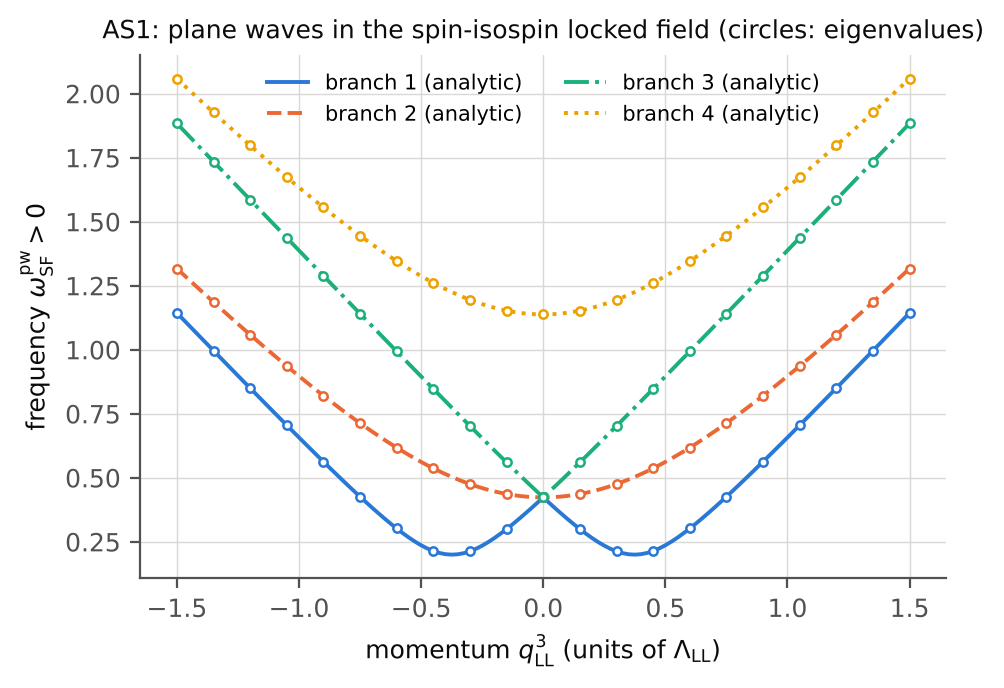
\includegraphics[width=0.88\textwidth,height=\textheight]{figures/fig_part1_s1_locked.png}

\textbf{Figure 1.} AS1: the four positive branches (7.4) of the plane
waves in the spin-isospin locked field (lines) and the eigenvalues of
\(\mathsf H^{\rm pw}_{\rm SF}\) (circles), for momenta along
\(x^3_{\rm LL}\); \(m_{\rm LL}=0.2\),
\(gw=g^{\rm v}_{\rm LL}w^{\rm lk}_{\rm SF}=0.747\). The branches of the
third component \(\pm1\) of the total of spin and isospin have their
minima at \(q^3_{\rm LL}=\mp gw/2\); at \(q^3_{\rm LL}=0\) three
branches meet (total 1). Data:
\texttt{data/part1\_s1\_locked\_dispersion.csv}.

\hypertarget{as2-landau-levels-in-a-constant-magnetic-field}{%
\subsection{7.2 AS2: Landau levels in a constant magnetic
field}\label{as2-landau-levels-in-a-constant-magnetic-field}}

Let the only gauge field be the magnetic field \(\mathcal B_{\rm SF}\)
of the direction \(W^3_{{\rm SF},p}\) along \(x^3_{\rm LL}\):
\(W^3_{{\rm SF},2}(x)=-\mathcal B_{\rm SF}\,x^1_{\rm LL}\) (lower index;
the three-vector potential has the component
\(\mathcal B_{\rm SF}x^1_{\rm LL}\) along \(x^2_{\rm LL}\), whose curl
is \(\mathcal B_{\rm SF}\) along \(x^3_{\rm LL}\)). An isospin component
of charge \(Q_{\rm LL}\) couples with the charge
\(e^{\rm c}_{\rm SF}=g^{\rm v}_{\rm LL}Q_{\rm LL}\). With plane waves
along \(x^2_{\rm LL}\) and \(x^3_{\rm LL}\) (momenta \(q^2_{\rm LL}\),
\(q^3_{\rm LL}\)), the equation for the four Dirac components of that
isospin component is \(\omega\Psi=\mathsf H\Psi\) with
\[\mathsf H=\alpha^1_{\rm LL}(-i\partial_1)+\alpha^2_{\rm LL}\big(q^2_{\rm LL}-e^{\rm c}_{\rm SF}\mathcal B_{\rm SF}x^1_{\rm LL}\big)+\alpha^3_{\rm LL}q^3_{\rm LL}+\beta_{\rm LL}m_{\rm LL}.\tag{7.5}\]
In the chirality blocks,
\(\mathsf H=\begin{pmatrix}-\vec\sigma\cdot\vec\pi&m_{\rm LL}\\m_{\rm LL}&\vec\sigma\cdot\vec\pi\end{pmatrix}\)
with
\(\vec\pi=(-i\partial_1,\,q^2_{\rm LL}-e^{\rm c}_{\rm SF}\mathcal B_{\rm SF}x^1_{\rm LL},\,q^3_{\rm LL})\),
so
\(\mathsf H^2=\mathrm{diag}((\vec\sigma\cdot\vec\pi)^2+m_{\rm LL}^2,\dots)\)
and
\((\vec\sigma\cdot\vec\pi)^2=\pi_1^2+\pi_2^2+(q^3_{\rm LL})^2+i\sigma^{\rm LL}_3[\pi_1,\pi_2]\)
with \(i[\pi_1,\pi_2]=-e^{\rm c}_{\rm SF}\mathcal B_{\rm SF}\).
\(\pi_1^2+\pi_2^2=-\partial_1^2+(e^{\rm c}_{\rm SF}\mathcal B_{\rm SF})^2(x^1_{\rm LL}-x_0)^2\),
\(x_0=q^2_{\rm LL}/(e^{\rm c}_{\rm SF}\mathcal B_{\rm SF})\), is a
harmonic oscillator with the eigenvalues
\(\lvert e^{\rm c}_{\rm SF}\mathcal B_{\rm SF}\rvert(2n+1)\),
\(n=0,1,2,\dots\); with \(\sigma^{\rm LL}_3=\pm1\) this gives the
\textbf{Landau levels}
\[\omega^2=m_{\rm LL}^2+(q^3_{\rm LL})^2+2n^{\rm L}_{\rm SF}\lvert e^{\rm c}_{\rm SF}\mathcal B_{\rm SF}\rvert,\qquad n^{\rm L}_{\rm SF}=0,1,2,\dots,\tag{7.6}\]
for both signs of \(\omega\); the level \(n^{\rm L}_{\rm SF}=0\) has one
spin state (spin along
\(\mathrm{sign}(e^{\rm c}_{\rm SF}\mathcal B_{\rm SF})\)), every higher
level two; the states are localized at \(x_0\) within the
\textbf{magnetic length}
\(\ell^{\rm B}_{\rm SF}=\lvert e^{\rm c}_{\rm SF}\mathcal B_{\rm SF}\rvert^{-1/2}\),
and each level is degenerate in \(q^2_{\rm LL}\). For
\(e^{\rm c}_{\rm SF}\mathcal B_{\rm SF}>0\) the lowest level is,
exactly,
\(\Psi=(\lambda_1\uparrow,\,\lambda_2\uparrow)\,\exp(-e^{\rm c}_{\rm SF}\mathcal B_{\rm SF}(x^1_{\rm LL}-x_0)^2/2)\)
(spin up in both blocks), with
\(\begin{pmatrix}-q^3_{\rm LL}&m_{\rm LL}\\m_{\rm LL}&q^3_{\rm LL}\end{pmatrix}\begin{pmatrix}\lambda_1\\\lambda_2\end{pmatrix}=\omega\begin{pmatrix}\lambda_1\\\lambda_2\end{pmatrix}\)
(\(\uparrow\) is the spin state \((1,0)\) of the two-component spinor
index), because
\(\pi_1+i\pi_2=-i(\partial_1+e^{\rm c}_{\rm SF}\mathcal B_{\rm SF}(x^1_{\rm LL}-x_0))\)
annihilates the Gaussian (\emph{check AS2-1}: the residual of
\(\mathsf H\Psi=\omega\Psi\) with exact derivatives at 41 points). In
the superfluid vacuum of Part II the field \(W^3_{{\rm SF},p}\) is the
massless photon and \(Q_{\rm LL}\) the electric charge: (7.6) are then
the Landau levels of the spinor charges in a magnetic field of the
photon. A magnetic field of \(B_{{\rm SF},p}\) gives the same with
\(e^{\rm c}_{\rm SF}=g^{\rm F}_{\rm LL}\).

\textbf{Lattice check.} With \(g^{\rm v}_{\rm LL}=1\),
\(\mathcal B_{\rm SF}=1\) (isospin up, \(e^{\rm c}_{\rm SF}=\tfrac12\))
and \(q^3_{\rm LL}=0.3\), the levels (7.6) are \(\omega=\)
\(0.3605551275\), \(1.063014581\), \(1.459451952\), \(1.769180601\) for
\(n^{\rm L}_{\rm SF}=0,1,2,3\). The Wilson lattice of Section 6.2 (open
ends, \(x^1_{\rm LL}\) from \(-10\) to \(10\)) reproduces the seven
lowest positive levels with their multiplicities, with the largest
relative deviations \(0.01953967595\), \(0.00969397194\),
\(0.004827511664\) at the spacings 0.1, 0.05, 0.025: the deviation
halves with the spacing, as expected for the Wilson term, and the
Richardson extrapolation \(2\omega(0.025)-\omega(0.05)\), which removes
the term of first order, agrees with (7.6) to
\(6.450238591\times10^{-5}\) (\emph{checks AS2-0 to AS2-4}; Figure 2).

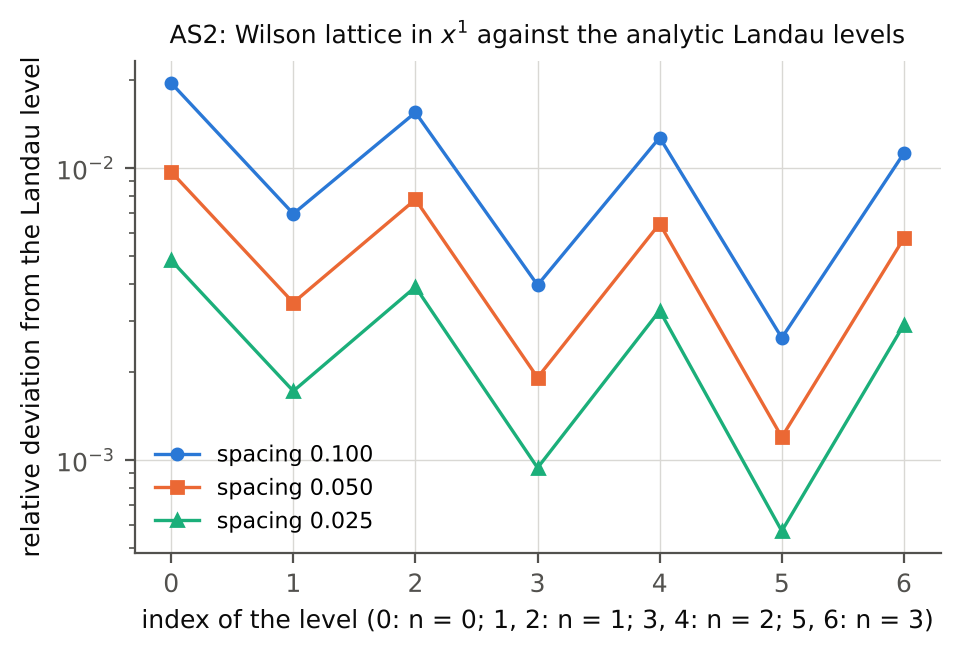
\includegraphics[width=0.82\textwidth,height=\textheight]{figures/fig_part1_s2_landau.png}

\textbf{Figure 2.} AS2: the relative deviation of the lattice levels
from the Landau levels (7.6), for the seven lowest positive levels
(index 0: \(n^{\rm L}_{\rm SF}=0\); 1 and 2: \(n^{\rm L}_{\rm SF}=1\);
3, 4: \(n^{\rm L}_{\rm SF}=2\); 5, 6: \(n^{\rm L}_{\rm SF}=3\)) and
three lattice spacings. Data: \texttt{data/part1\_s2\_landau.csv}.

\hypertarget{as3-the-uniform-superfluid-of-the-spin-zero-pairing-mean-field}{%
\subsection{7.3 AS3: the uniform superfluid of the spin-zero pairing
(mean
field)}\label{as3-the-uniform-superfluid-of-the-spin-zero-pairing-mean-field}}

Keep, of the self-interaction \(V^{(1)}_{\rm SF}\), only the pairing
term, and of its Wick contractions (6.2) only the pair contraction (the
pairing-only, or BCS, approximation; Part II keeps all terms). A uniform
state at the chemical potential \(\mu_{\rm LL}\) (the term
\(-\mu_{\rm LL}\Psi^\dagger\Psi\) is added to \(\mathcal H_{\rm SF}\))
with the order parameter \(\vec d_{\rm LL}\) has the self-energies
\(\mathsf N_{\rm SF}=0\) and
\(\mathsf P_{\rm SF}=\mathsf P_{\rm LL}=\sum_\iota d^\iota_{\rm LL}(\mathsf K^\iota_{\rm LL})^\dagger\),
and (6.5) becomes the Bogoliubov-de Gennes matrix
\(\mathsf H_{\rm LL}(\vec q_{\rm LL})\) with the blocks
\(\mathsf h_{\rm LL}(\vec q_{\rm LL})-\mu_{\rm LL}\),
\(\mathsf P_{\rm LL}\), \(\mathsf P_{\rm LL}^\dagger\) and
\(-(\mathsf h_{\rm LL}(-\vec q_{\rm LL})-\mu_{\rm LL})^T\).

\textbf{The spectrum.} Two identities make it explicit. (i)
\(\mathsf h_{\rm LL}(\vec q)(\mathsf K^\iota)^\dagger=(\mathsf K^\iota)^\dagger\mathsf h_{\rm LL}(-\vec q)^T\):
the isospin part of
\((\mathsf K^\iota)^\dagger=\mathrm{diag}(\mathsf E,\mathsf E)\otimes(\mathsf E\tau_\iota)^\dagger\)
commutes with \(\mathsf h_{\rm LL}\); \(\beta_{\rm LL}\) commutes with
\(\mathrm{diag}(\mathsf E,\mathsf E)\); and
\(\alpha^j\mathrm{diag}(\mathsf E,\mathsf E)=-\mathrm{diag}(\mathsf E,\mathsf E)(\alpha^j)^T\)
because \(\mathsf E(\sigma^{\rm LL}_j)^T=-\sigma^{\rm LL}_j\mathsf E\).
Hence the off-diagonal blocks of \(\mathsf H_{\rm LL}^2\) vanish. (ii)
\(\mathsf P_{\rm LL}\mathsf P_{\rm LL}^\dagger=\mathsf 1_4\otimes\sum_{\iota\iota'}d^\iota_{\rm LL}(d^{\iota'}_{\rm LL})^*\tau_\iota\tau_{\iota'}=\lvert\vec d_{\rm LL}\rvert^2+i(\vec d_{\rm LL}\times\vec d^{\,*}_{\rm LL})\cdot\vec\tau\),
whose eigenvalues are
\((\Delta^\pm_{\rm LL})^2=\lvert\vec d_{\rm LL}\rvert^2(1\pm\zeta_{\rm LL})\)
with
\(\zeta_{\rm LL}=\lvert\vec d_{\rm LL}\times\vec d^{\,*}_{\rm LL}\rvert/\lvert\vec d_{\rm LL}\rvert^2\).
For a \textbf{unitary} state,
\(\vec d_{\rm LL}=\Delta_{\rm LL}e^{i\phi}\vec n\) with a real unit
vector \(\vec n\) (\(\zeta_{\rm LL}=0\); the \textbf{polar} states),
\(\mathsf H_{\rm LL}^2=\mathrm{diag}((\mathsf h-\mu)^2+\Delta^2_{\rm LL},\dots)\)
and the sixteen eigenvalues are
\[\pm E^+_{\rm LL},\ \pm E^-_{\rm LL}\ \text{(each four times)},\qquad E^\pm_{\rm LL}=\big[(\varepsilon_{\rm LL}\pm\mu_{\rm LL})^2+\Delta_{\rm LL}^2\big]^{1/2}\tag{7.7}\]
(\emph{check AS3-1}, 100 random momenta, chemical potentials, gaps,
phases and directions).

\textbf{The energy and the gap equation.} The ground state of the
mean-field Hamiltonian
\(\tfrac12\sum_{\vec q}\mathcal N_{\rm LL}^\dagger\mathsf H_{\rm LL}\mathcal N_{\rm LL}\)
plus the constant \(V\lvert\vec d_{\rm LL}\rvert^2/G_{\rm LL}\) (which
is what remains of \(-\tfrac14G_{\rm LL}\sum\Pi^\dagger\Pi\) after the
decoupling
\(\Pi^\dagger\Pi\to\langle\Pi\rangle^*\Pi+\Pi^\dagger\langle\Pi\rangle-\lvert\langle\Pi\rangle\rvert^2\))
has the energy per volume, at \(\mu_{\rm LL}=0\) and measured from the
normal vacuum,
\[\mathcal E^{\rm MF}_{\rm SF}(\Delta_{\rm LL})=-\frac2{\pi^2}\Big[I^{(3)}_{\rm SF}\big(M^{\rm q}_{\rm LL}\big)-I^{(3)}_{\rm SF}\big(m_{\rm LL}\big)\Big]+\frac{\Delta_{\rm LL}^2}{G_{\rm LL}},\qquad M^{\rm q}_{\rm LL}=\big(m_{\rm LL}^2+\Delta_{\rm LL}^2\big)^{1/2},\tag{7.8}\]
with the integrals over the momenta below the cutoff
\[\begin{aligned}I^{(1)}_{\rm SF}(M^{\rm q}_{\rm LL})&=\int_0^{\Lambda_{\rm LL}}\frac{q^2\,dq}{(q^2+(M^{\rm q}_{\rm LL})^2)^{1/2}}=\tfrac12\Big[\Lambda_{\rm LL}\big(\Lambda_{\rm LL}^2+(M^{\rm q}_{\rm LL})^2\big)^{1/2}-(M^{\rm q}_{\rm LL})^2\,\mathrm{arsinh}\frac{\Lambda_{\rm LL}}{M^{\rm q}_{\rm LL}}\Big],\\I^{(3)}_{\rm SF}(M^{\rm q}_{\rm LL})&=\int_0^{\Lambda_{\rm LL}}q^2\big(q^2+(M^{\rm q}_{\rm LL})^2\big)^{1/2}dq\\&=\tfrac18\Big[\Lambda_{\rm LL}\big(2\Lambda_{\rm LL}^2+(M^{\rm q}_{\rm LL})^2\big)\big(\Lambda_{\rm LL}^2+(M^{\rm q}_{\rm LL})^2\big)^{1/2}-(M^{\rm q}_{\rm LL})^4\,\mathrm{arsinh}\frac{\Lambda_{\rm LL}}{M^{\rm q}_{\rm LL}}\Big]\end{aligned}\]
(\(I^{(1)}_{\rm SF}(m_{\rm LL})\) and \(I^{(3)}_{\rm SF}(m_{\rm LL})\)
are the same with \(m_{\rm LL}\) in place of \(M^{\rm q}_{\rm LL}\)).
Derivation: each momentum contributes \(-\tfrac12\) times the sum of the
eight positive eigenvalues, \(-4E\) with
\(E=(q^2+(M^{\rm q}_{\rm LL})^2)^{1/2}\) at \(\mu_{\rm LL}=0\), and
\(\int d^3q/(2\pi)^3=(2\pi^2)^{-1}\int q^2dq\). Since
\(dI^{(3)}_{\rm SF}/d\Delta_{\rm LL}=\Delta_{\rm LL}I^{(1)}_{\rm SF}\),
the stationary points of (7.8) are \(\Delta_{\rm LL}=0\) and the
solutions of the \textbf{gap equation}
\[1=\frac{G_{\rm LL}}{\pi^2}\,I^{(1)}_{\rm SF}\big(M^{\rm q}_{\rm LL}\big).\tag{7.9}\]
Because \(I^{(1)}_{\rm SF}\) decreases with its argument, (7.9) has a
solution exactly when
\(G_{\rm LL}>G^{\rm crit}_{\rm LL}=\pi^2/I^{(1)}_{\rm SF}(m_{\rm LL})=21.28660976\).
For \(G_{\rm LL}=22.5\) the solution is
\(\Delta_{\rm LL}=0.2094933033\), the quasi-particle mass
\(M^{\rm q}_{\rm LL}=0.2896332925\) (the gap of the single
quasi-particle), and
\(\mathcal E^{\rm MF}_{\rm SF}=-5.288449106\times10^{-5}<0\): the
condensed state lies below the normal vacuum. (\emph{Checks AS3-2 to
AS3-4}: (7.8) against Gauss-Legendre quadrature of the eigenvalues of
\(\mathsf H_{\rm LL}\), the stationarity at the solution of (7.9), and
the values; the Python program finds the same gap with a different root
finder.)

\textbf{Polar or non-unitary?} For a fixed
\(\lvert\vec d_{\rm LL}\rvert\), a non-unitary state has the two gaps
\(\Delta^\pm_{\rm LL}\), and the energy contains
\(-[(\varepsilon^2+(\Delta^+)^2)^{1/2}+(\varepsilon^2+(\Delta^-)^2)^{1/2}]\)
in place of \(-2(\varepsilon^2+\lvert\vec d\rvert^2)^{1/2}\); since the
square root is concave and
\((\Delta^+)^2+(\Delta^-)^2=2\lvert\vec d\rvert^2\), the former is
larger: in this approximation the polar states have the lowest energy.
Their manifold is described by the phase \(\phi\) and the direction
\(\vec n\) (with \((\phi,\vec n)\) and \((\phi+\pi,-\vec n)\) the same
state). Figure 3 shows the energy along one direction: for
\(G_{\rm LL}>G^{\rm crit}_{\rm LL}\) the normal vacuum
\(\Delta_{\rm LL}=0\) is a local maximum and the minima lie at
\(\pm\Delta_{\rm LL}\), the cut of a ``Mexican hat''; Part III takes
this up with all terms of the potential.

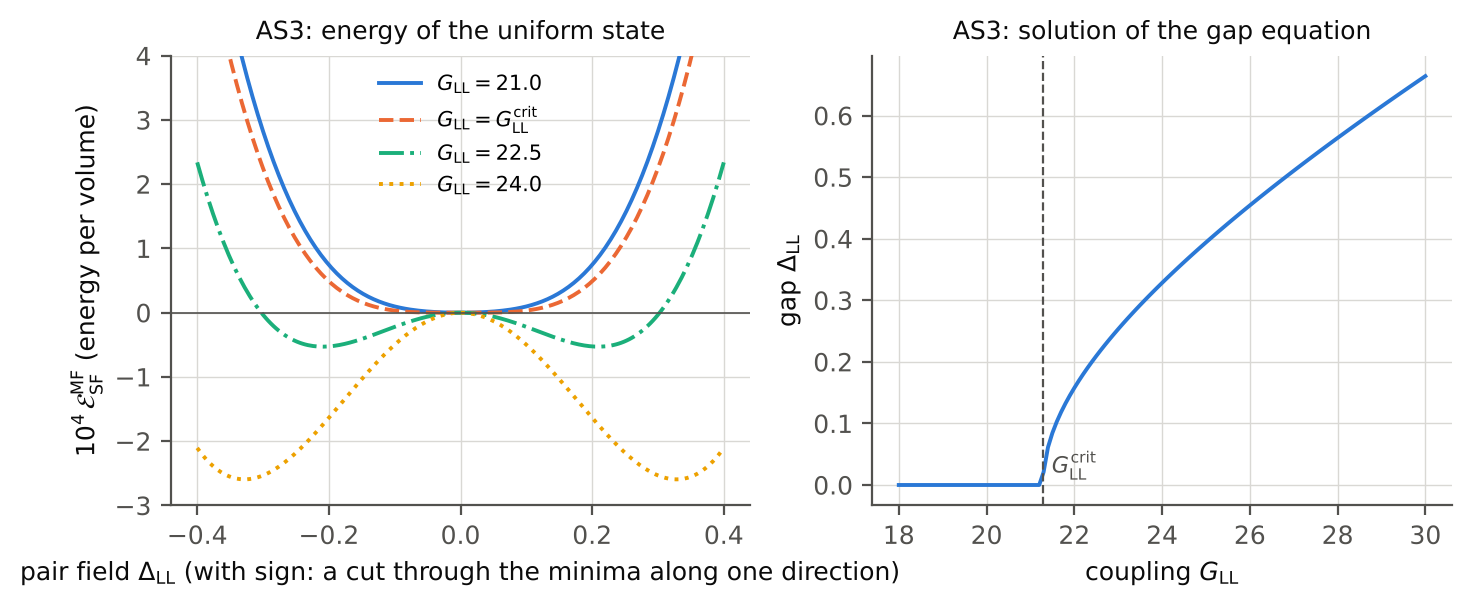
\includegraphics[width=1\textwidth,height=\textheight]{figures/fig_part1_s3_superfluid.png}

\textbf{Figure 3.} AS3. Left: the energy per volume (7.8) of the polar
state as a function of the signed pair field, for four couplings; for
\(G_{\rm LL}\le G^{\rm crit}_{\rm LL}\) the minimum is the normal
vacuum, for \(G_{\rm LL}>G^{\rm crit}_{\rm LL}\) two minima appear at
\(\pm\Delta_{\rm LL}\). Right: the solution of the gap equation (7.9);
it rises from 0 at \(G^{\rm crit}_{\rm LL}\). Data:
\texttt{data/part1\_s3\_energy.csv}, \texttt{data/part1\_s3\_gap.csv}.

\hypertarget{as4-the-kink-of-the-pair-field-and-its-bound-states}{%
\subsection{7.4 AS4: the kink of the pair field and its bound
states}\label{as4-the-kink-of-the-pair-field-and-its-bound-states}}

Let the pair field depend on \(x^1_{\rm LL}\) and change sign:
\(\vec d_{\rm LL}(x)=\Delta^\infty_{\rm LL}\tanh(x^1_{\rm LL}/\ell^{\rm K}_{\rm LL})\,\vec e_3\)
(\(\vec e_3\) the unit vector of the third isospin direction), a domain
wall of the polar superfluid of width \(\ell^{\rm K}_{\rm LL}\) between
the vacua \(-\Delta^\infty_{\rm LL}\) and \(+\Delta^\infty_{\rm LL}\)
(equivalent to a jump of the phase by \(\pi\)). At \(\mu_{\rm LL}=0\)
and \(q^2_{\rm LL}=q^3_{\rm LL}=0\) the Bogoliubov-de Gennes operator of
the quasi-particles in this field, the operator of (6.5) in which
\(\vec q_{\rm LL}\) becomes \(-i\partial_1\), is
\[\begin{aligned}\mathsf H^{\rm K}_{\rm SF}&=-i\mathsf A^{\rm K}_{\rm SF}\partial_1+\Delta_{\rm LL}(x)\,\mathsf P^{\rm K}_{\rm SF}+m_{\rm LL}\mathsf B^{\rm K}_{\rm SF},\\\mathsf A^{\rm K}_{\rm SF}&=\mathrm{diag}\big(\alpha^1_{\rm LL},(\alpha^1_{\rm LL})^*\big),\qquad\mathsf P^{\rm K}_{\rm SF}=\begin{pmatrix}0&(\mathsf K^3_{\rm LL})^\dagger\\\mathsf K^3_{\rm LL}&0\end{pmatrix},\qquad\mathsf B^{\rm K}_{\rm SF}=\mathrm{diag}(\beta_{\rm LL},-\beta_{\rm LL})\end{aligned}\tag{7.10}\]
(\(16\times16\) matrices of \(8\times8\) blocks; the lower right block
of (6.5), \(-(\mathsf h(-\vec q))^T\), becomes \(-\mathsf h^*\) in
\(x\), which gives \(-i(\alpha^1)^*\partial_1-\beta m\)).
\textbf{Structure.} The three matrices anticommute pairwise and square
to \(\mathsf 1_{16}\) (\emph{check AS4-1}). Hence, with
\(\mathsf H^{{\rm K},0}_{\rm SF}=\mathsf H^{\rm K}_{\rm SF}-m_{\rm LL}\mathsf B^{\rm K}_{\rm SF}\),
\((\mathsf H^{\rm K}_{\rm SF})^2=(\mathsf H^{{\rm K},0}_{\rm SF})^2+m_{\rm LL}^2\)
and
\[\big(\mathsf H^{{\rm K},0}_{\rm SF}\big)^2=-\partial_1^2+\Delta_{\rm LL}(x)^2+\mathsf G^{\rm K}_{\rm SF}\,\Delta_{\rm LL}'(x),\qquad\mathsf G^{\rm K}_{\rm SF}=-i\mathsf A^{\rm K}_{\rm SF}\mathsf P^{\rm K}_{\rm SF},\tag{7.11}\]
(the cross terms give
\(-i\mathsf A\mathsf P\,\partial_1(\Delta\,\cdot)-i\Delta\mathsf P\mathsf A\,\partial_1=-i\mathsf A\mathsf P\Delta'\)).
\(\mathsf G^{\rm K}_{\rm SF}\) is Hermitian, squares to 1, has the
eigenvalues \(\pm1\) eight times each and commutes with
\(\mathsf B^{\rm K}_{\rm SF}\) (\emph{check AS4-2}). On its eigenspace
\(-1\), with
\(s^{\rm K}_{\rm SF}=\Delta^\infty_{\rm LL}\ell^{\rm K}_{\rm LL}\),
(7.11) is the Pöschl-Teller operator
\(-\partial_1^2+(\Delta^\infty_{\rm LL})^2-s^{\rm K}_{\rm SF}(s^{\rm K}_{\rm SF}+1)(\ell^{\rm K}_{\rm LL})^{-2}\,\mathrm{sech}^2(x^1_{\rm LL}/\ell^{\rm K}_{\rm LL})\),
whose bound states have the eigenvalues
\((\Delta^\infty_{\rm LL})^2-(s^{\rm K}_{\rm SF}-n)^2/(\ell^{\rm K}_{\rm LL})^2\),
\(n=0,1,\dots\), \(n<s^{\rm K}_{\rm SF}\); on the eigenspace \(+1\) the
same with \(s^{\rm K}_{\rm SF}-1\) in place of \(s^{\rm K}_{\rm SF}\),
which gives the same eigenvalues for \(n\ge1\). The bound states of the
quasi-particles therefore have the energies
\[\pm\big(m_{\rm LL}^2+(E^{\rm K}_{{\rm SF},n})^2\big)^{1/2},\qquad(E^{\rm K}_{{\rm SF},n})^2=(\Delta^\infty_{\rm LL})^2-\big(\Delta^\infty_{\rm LL}-n/\ell^{\rm K}_{\rm LL}\big)^2,\qquad n=0,1,\dots,\ n<s^{\rm K}_{\rm SF},\tag{7.12}\]
below the continuum, which begins at
\((m_{\rm LL}^2+(\Delta^\infty_{\rm LL})^2)^{1/2}\). The state \(n=0\)
is the zero mode of the kink of the massless problem (Jackiw-Rebbi),
\(\chi^{\rm K}_{\rm SF}\varphi^{\rm K}_{{\rm SF},0}(x)\) with
\(\varphi^{\rm K}_{{\rm SF},0}=\mathrm{sech}^{s^{\rm K}_{\rm SF}}(x^1_{\rm LL}/\ell^{\rm K}_{\rm LL})\)
and a constant spinor \(\chi^{\rm K}_{\rm SF}\) of the eigenspace
\(\mathsf G^{\rm K}_{\rm SF}=-1\) (there
\(\mathsf P\chi=-i\mathsf A\chi\), so
\(\mathsf H^{{\rm K},0}(\chi\varphi)=-i\mathsf A\chi(\varphi'+\Delta\varphi)=0\));
the Dirac mass lifts it to \(\pm m_{\rm LL}\), four states of each sign
(the eigenvalues of \(\mathsf B^{\rm K}_{\rm SF}\) on that eigenspace,
\emph{check AS4-2b}): \textbf{the domain wall binds fermionic
quasi-particles inside the gap, at the energy \(m_{\rm LL}\).} The state
\(n=1\) is built from
\(\varphi^{\rm K}_{{\rm SF},1}=\mathrm{sech}^{s^{\rm K}_{\rm SF}-1}(x^1_{\rm LL}/\ell^{\rm K}_{\rm LL})\tanh(x^1_{\rm LL}/\ell^{\rm K}_{\rm LL})\):
with \(u=\chi\varphi^{\rm K}_{{\rm SF},1}\) (\(\chi\) in the eigenspace
\(-1\)), \(\Psi_0=\mathsf H^{{\rm K},0}u+E^{\rm K}_{{\rm SF},1}u\) is an
eigenvector of \(\mathsf H^{{\rm K},0}\) with the eigenvalue
\(E^{\rm K}_{{\rm SF},1}\); \(\mathsf B^{\rm K}\) maps it to the
eigenvalue \(-E^{\rm K}_{{\rm SF},1}\), and on the pair
\((\Psi_0,\mathsf B\Psi_0)\) the operator \(\mathsf H^{\rm K}\) acts as
\(\begin{pmatrix}E^{\rm K}_{{\rm SF},1}&m_{\rm LL}\\m_{\rm LL}&-E^{\rm K}_{{\rm SF},1}\end{pmatrix}\),
whose eigenvector
\(\Psi_0+\frac{E-E^{\rm K}_{{\rm SF},1}}{m_{\rm LL}}\mathsf B\Psi_0\)
has the eigenvalue
\(E=(m_{\rm LL}^2+(E^{\rm K}_{{\rm SF},1})^2)^{1/2}\).

With \(\Delta^\infty_{\rm LL}=0.5\) and \(\ell^{\rm K}_{\rm LL}=4\)
(\(s^{\rm K}_{\rm SF}=2\)): the bound states are at
\(\pm m_{\rm LL}=\pm0.2\) and \(\pm0.4769696007\)
(\((E^{\rm K}_{{\rm SF},1})^2=0.1875\)), the continuum begins at
\(0.5385164807\). \emph{Checks:} AS4-3 and AS4-4 evaluate
\((\mathsf H^{\rm K}-E)\Psi\) for the analytic states \(n=0\) and
\(n=1\) with exact derivatives at 61 points (residuals at the level of
rounding); AS4-5 and AS4-6 compute the spectrum on the Wilson lattice of
Section 6.2. On the lattice the problem reduces exactly to two
components: the algebra of three anticommuting matrices that square to 1
has two inequivalent irreducible representations of dimension 2, so in a
suitable basis (7.10) is eight copies of
\(\sigma^{\rm LL}_1(-i\partial_1)+\sigma^{\rm LL}_2\Delta_{\rm LL}(x)\pm\sigma^{\rm LL}_3m_{\rm LL}\);
the lattice of this operator has exactly three bound states below the
continuum, \(-m_{\rm LL}\) and
\(\pm(m_{\rm LL}^2+(E^{\rm K}_{{\rm SF},1})^2)^{1/2}\), for the spacings
0.1, 0.05 and 0.025 (relative deviations \(0.01241095554\),
\(0.006227620264\), \(0.003119390085\)), and the Richardson
extrapolation agrees with (7.12) to \(1.11599057\times10^{-5}\) (Figure
4).

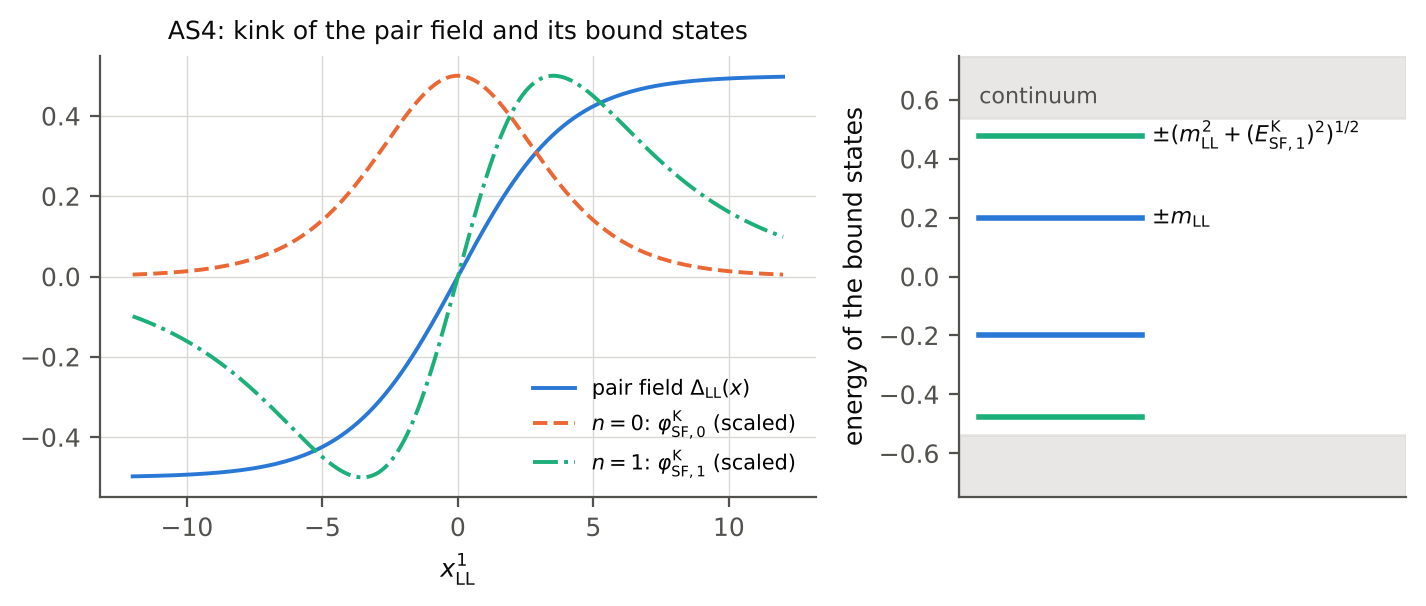
\includegraphics[width=1\textwidth,height=\textheight]{figures/fig_part1_s4_kink.png}

\textbf{Figure 4.} AS4. Left: the kink \(\Delta_{\rm LL}(x)\) of the
pair field (\(\Delta^\infty_{\rm LL}=0.5\), \(\ell^{\rm K}_{\rm LL}=4\))
and the profiles of its bound states \(n=0\) (\(\mathrm{sech}^2\)) and
\(n=1\) (\(\mathrm{sech}\,\tanh\)), scaled. Right: the energies of the
bound states, \(\pm m_{\rm LL}\) and
\(\pm(m_{\rm LL}^2+(E^{\rm K}_{{\rm SF},1})^2)^{1/2}\), below the
continuum (grey). Data: \texttt{data/part1\_s4\_kink\_profiles.csv},
\texttt{data/part1\_s4\_kink\_lattice.csv}.

\hypertarget{summary-of-the-analytic-solutions}{%
\subsection{7.5 Summary of the analytic
solutions}\label{summary-of-the-analytic-solutions}}

\sptkeptpenalty=10000
\begin{longtable}[]{@{}
  >{\raggedright\arraybackslash}p{(\columnwidth - 6\tabcolsep) * \real{0.2500}}
  >{\raggedright\arraybackslash}p{(\columnwidth - 6\tabcolsep) * \real{0.2500}}
  >{\raggedright\arraybackslash}p{(\columnwidth - 6\tabcolsep) * \real{0.2500}}
  >{\raggedright\arraybackslash}p{(\columnwidth - 6\tabcolsep) * \real{0.2500}}@{}}
\toprule\noalign{}
\begin{minipage}[b]{\linewidth}\raggedright
case
\end{minipage} & \begin{minipage}[b]{\linewidth}\raggedright
equation solved
\end{minipage} & \begin{minipage}[b]{\linewidth}\raggedright
result
\end{minipage} & \begin{minipage}[b]{\linewidth}\raggedright
checks
\end{minipage} \\
\midrule\noalign{}
\endhead
\bottomrule\noalign{}
\endlastfoot
AS1 plane waves & (5.5) without self-interaction, constant gauge fields
& (7.1); (7.2) abelian; (7.3), (7.4) spin-isospin locked field & AS1-1
to AS1-5 \\*
AS2 Landau levels & (5.5) without self-interaction, constant magnetic
field & (7.6), lowest level explicit & AS2-0 to AS2-4 \\*
AS3 uniform superfluid & mean field (6.6), stationary, pairing only &
spectrum (7.7), energy (7.8), gap equation (7.9) & AS3-1 to AS3-4 \\*
AS4 kink & mean field of the quasi-particles in the pair field
\(\Delta^\infty_{\rm LL}\tanh(x^1_{\rm LL}/\ell^{\rm K}_{\rm LL})\) &
bound states (7.12) at \(\pm m_{\rm LL}\) and above & AS4-1 to AS4-6 \\
\end{longtable}

\hypertarget{provenance-of-part-i-programs-commands-reports-data-and-figures}{%
\section{8. Provenance of part I: programs, commands, reports, data and
figures}\label{provenance-of-part-i-programs-commands-reports-data-and-figures}}

\hypertarget{the-programs-and-how-to-run-them}{%
\subsection{8.1 The programs and how to run
them}\label{the-programs-and-how-to-run-them}}

All paths are relative to the folder
\texttt{Revision\_HS\_CJT\_and\_Kohn-Sham} of PROJECT spacetimes.

\begin{itemize}
\item
  \textbf{Rust} (requires the Rust toolchain with \texttt{cargo}; no
  crate is downloaded). The workspace \texttt{rust/} contains the
  library \texttt{sfcore} (bi-quaternions and bi-octonions, Dirac
  matrices, automatic differentiation, Fock-space operators, the
  block-tridiagonal eigenvalue solver, quadrature, reports) and the
  program \texttt{sf\_part1} (crate \texttt{rust/sfpart1}), which runs
  the checks A, F, C, E and S of this part and writes the data files:

\begin{verbatim}
cd rust
cargo build --release
./target/release/sf_part1
\end{verbatim}

  Output: \texttt{data/hck\_part1\_checks.txt} (the report),
  \texttt{data/part1\_values.csv} (the numbers printed in Section 7),
  and the data of the figures. The program ends with the exit status 0
  exactly when every check passes.
\item
  \textbf{Python} (requires Python 3 with numpy, scipy, sympy and
  matplotlib). \texttt{python/sf\_part1.py} is an independent second
  computation of the checks (other random test values; finite
  differences of eighth order instead of automatic differentiation;
  LAPACK instead of the Rust eigensolvers; symbolic Euler-Lagrange
  equations with sympy); \texttt{python/sf\_part1\_figures.py} draws the
  four figures from the data of the Rust program:

\begin{verbatim}
python3 python/sf_part1.py
python3 python/sf_part1_figures.py
\end{verbatim}
\item
  \textbf{Documents.} \texttt{code/scripts/write\_part1\_fragments.py}
  turns the reports and values into the tables and numbers of this
  manuscript; \texttt{code/scripts/assemble\_docs.py} writes the
  Markdown from its source \texttt{docs\_src/superfluid.src.md}, and
  \texttt{code/scripts/build\_docs.sh} makes the \texttt{.tex} (pandoc)
  and the \texttt{.pdf} (XeLaTeX):

\begin{verbatim}
python3 code/scripts/write_part1_fragments.py
python3 code/scripts/assemble_docs.py docs_src/superfluid.src.md
bash code/scripts/build_docs.sh superfluid.md
\end{verbatim}
\end{itemize}

\hypertarget{the-report-of-the-rust-program}{%
\subsection{8.2 The report of the Rust
program}\label{the-report-of-the-rust-program}}

\begin{longtable}[]{@{}
  >{\raggedright\arraybackslash}p{(\columnwidth - 8\tabcolsep) * \real{0.2000}}
  >{\raggedright\arraybackslash}p{(\columnwidth - 8\tabcolsep) * \real{0.2000}}
  >{\raggedright\arraybackslash}p{(\columnwidth - 8\tabcolsep) * \real{0.2000}}
  >{\raggedright\arraybackslash}p{(\columnwidth - 8\tabcolsep) * \real{0.2000}}
  >{\raggedright\arraybackslash}p{(\columnwidth - 8\tabcolsep) * \real{0.2000}}@{}}
\toprule\noalign{}
\begin{minipage}[b]{\linewidth}\raggedright
check
\end{minipage} & \begin{minipage}[b]{\linewidth}\raggedright
result
\end{minipage} & \begin{minipage}[b]{\linewidth}\raggedright
deviation
\end{minipage} & \begin{minipage}[b]{\linewidth}\raggedright
tolerance
\end{minipage} & \begin{minipage}[b]{\linewidth}\raggedright
statement
\end{minipage} \\
\midrule\noalign{}
\endhead
\bottomrule\noalign{}
\endlastfoot
A-1 & PASS & 0.000e0 & 0.0e0 & quaternion units: e\_j\^{}2 = -1, e\_j
e\_k = -e\_k e\_j = e\_l for (j,k,l) cyclic \\
A-2 & PASS & 0.000e0 & 0.0e0 & bi-octonion units: e\_p\^{}2 = -1, e\_p
e\_q = -e\_q e\_p (p != q, both \textgreater= 1), e\_j e\_4 =
e\_\{4+j\} \\
A-3 & PASS & 0.000e0 & 0.0e0 & the complex norm is multiplicative, N(xy)
= N(x)N(y), 200 random bi-octonions (exact integers) \\
A-4 & PASS & 0.000e0 & 0.0e0 & x xbar = N(x) e\_0, 200 random
bi-octonions (exact) \\
A-5 & PASS & 0.000e0 & 0.0e0 & alternativity (xx)y = x(xy), (yx)x =
y(xx), 200 random triples (exact) \\
A-6 & PASS & 0.000e0 & 0.0e0 & the three Moufang identities, 200 random
triples (exact) \\
A-7 & PASS & -- & -- & the bi-octonion product is not associative: (e1
e2) e4 - e1 (e2 e4) = 2 e7, and of the 343 triples of imaginary units
168 have a nonzero associator; the largest associator of the 200 random
triples is nonzero (nonzero unit associators 168 of 343; (e1e2)e4 -
e1(e2e4) = 2 e7: true; max random associator 654.638831723264) \\
A-8 & PASS & 1.776e-15 & 1.0e-13 & bi-quaternions: associative; M(bb') =
M(b)M(b'); det M(b) = N(b); M(b\^{}dag) = M(b)\^{}dag; the inverse map
recovers b (200 random) \\
A-9 & PASS & 0.000e0 & 1.0e-13 & M31: the points are Hermitian
bi-quaternions (x\^{}dag = x), M(x) = sum\_p x\^{}p sigma\_p, N(x) =
Minkowski interval (200 random) \\
A-10a & PASS & 3.324e-14 & 1.0e-11 & x -\textgreater{} g x g\^{}dag maps
M31 to itself (Hermitian image) and keeps N(x) (200 random unit g) \\
A-10b & PASS & 5.551e-15 & 1.0e-10 & L(g)\^{}T eta L(g) = eta and det
L(g) = 1 (200 random unit g) \\
A-10c & PASS & -- & -- & L(g)\_00 \textgreater= 1 (orthochronous) for
the 200 random unit g (all 200) \\
A-10d & PASS & 4.441e-15 & 1.0e-10 & L(gh) = L(g) L(h) and L(-g) = L(g)
(200 random pairs) \\
A-11 & PASS & 0.000e0 & 1.0e-15 & the 27 commutators of the generators:
{[}J\^{}j,J\^{}k{]} = eps\_jkl J\^{}l, {[}J\^{}j,K\^{}k{]} = eps\_jkl
K\^{}l, {[}K\^{}j,K\^{}k{]} = -eps\_jkl J\^{}l \\
A-12 & PASS & 0.000e0 & 0.0e0 & spinor charges: (b e4) g = (b gbar) e4,
g (b e4) = (b g) e4, (v ((b e4) e4)) e4\^{}-1 = (v b) e4 (200 random,
exact) \\
F-1 & PASS & 0.000e0 & 0.0e0 & the eight components at one point:
\{Psi\_c, Psi\_c'\^{}dag\} = delta, \{Psi\_c, Psi\_c'\} = 0 (Fock space
of dimension 256) \\
F-2 & PASS & 0.000e0 & 1.0e-15 & Dirac matrices: \{g\^{}p, g\^{}q\} = 2
eta\^{}pq, g\^{}0 g\^{}p g\^{}0 = (g\^{}p)\^{}dag, C g\^{}p C\^{}-1 =
-(g\^{}p)\^{}T, g\^{}ch = diag(-1,-1,1,1), C = diag(E,-E), C\^{}T =
-C \\
F-3a & PASS & 1.599e-14 & 1.0e-10 & S(g)\^{}-1 g\^{}p S(g) = sum\_q
L(g)\_pq g\^{}q (200 random unit g) \\
F-3b & PASS & 6.280e-16 & 1.0e-10 & S(g)\^{}dag g\^{}0 S(g) = g\^{}0, so
Psi-bar Psi is invariant (200 random) \\
F-3c & PASS & 7.229e-15 & 1.0e-10 & S(gh) = S(g) S(h) and S(-g) = -S(g)
(200 random pairs) \\
F-3d & PASS & 3.625e-15 & 1.0e-10 & the Dirac matrices of the frame
gtilde f gtilde\^{}dag are S(g) g\^{}p S(g)\^{}-1 (200 random) \\
F-4 & PASS & 5.674e-15 & 1.0e-12 & spinor charges: psi'(b gbar) = M(g)
psi'(b), psi'(b g\^{}dag) = M(gtilde) psi'(b), psi'(v b) = psi'(b)
M(v)\^{}T with M(v) in SU(2) (200 random) \\
F-5a & PASS & 0.000e0 & 1.0e-14 & D1: the three Pauli-Guersey generators
commute with the six Lorentz generators on (psi, psi\^{}dag) \\
F-5b & PASS & 0.000e0 & 1.0e-14 & D1: they commute with the massless
Dirac Hamiltonian at 50 random momenta (the kinetic term is
invariant) \\
F-5c & PASS & -- & -- & D1: the Lorentz-invariant antisymmetric
bilinears of one point form a complex space of dimension 6; of these
none (dimension 0) is invariant under the Pauli-Guersey SU(2): no
GEE-invariant mass term of a single Dirac field (dimension of the
Lorentz invariants 6, of the GEE invariants 0) \\
F-5d & PASS & -- & -- & D1: with the mass m = 0.2 the Pauli-Guersey
generators do not commute with the Dirac Hamiltonian (smallest of the
largest commutators over 50 momenta \textgreater{} 0.1) (0.200000) \\
F-6 & PASS & 0.000e0 & 1.0e-13 & doublet: {[}m Psi-bar Psi, T\^{}iota{]}
= {[}m Psi-bar Psi, F{]} = {[}m Psi-bar Psi, J\^{}j{]} = 0 on the Fock
space of one point \\
F-7a & PASS & 1.650e-15 & 1.0e-12 & pair matrices: K\^{}T = -K, K\^{}dag
K = 1, (S (x) 1)\^{}T K (S (x) 1) = K (50 random g), (1 (x) U)\^{}T
K\^{}a (1 (x) U) = sum\_b R(U)\_ab K\^{}b (50 random U), for the six
K\^{}iota, K'\^{}iota \\
F-7b & PASS & -- & -- & the Lorentz-invariant antisymmetric pair
matrices of the eight components form a space of dimension 6 (the
spin-zero pairs are isospin triplets) (dimension 6) \\
C-1 & PASS & 5.551e-16 & 1.0e-12 & SU(2)\_v x U(1)\^{}F: nabla'\_p
(e\^{}\{i theta\} U Psi) = e\^{}\{i theta\} U nabla\_p Psi with W' = U W
U\^{}dag + (i/g)(dU)U\^{}dag, B' = B - (d theta)/g\_F (12 points, 4
directions) \\
C-2 & PASS & 2.236e-16 & 1.0e-13 & the transformed W'\_p is again
Hermitian and traceless: real components W'\^{}iota\_p \\
C-3 & PASS & 2.238e-16 & 1.0e-12 & field strengths: W'\_pq = U W\_pq
U\^{}dag, B'\_pq = B\_pq, and W\^{}iota\_pq = dW - dW - g eps W W \\
C-4 & PASS & 9.037e-16 & 1.0e-12 & isotriplet of fermion number 2: nabla
Phi = dPhi - g W x Phi + 2 i g\_F B Phi is covariant, Phi' = e\^{}\{2 i
theta\} R(U) Phi; R(U) orthogonal \\
C-5 & PASS & 5.551e-16 & 1.0e-11 & the Yang-Mills operator D\_q W\^{}\{q
p\} is covariant (adjoint): D'\_q W'\^{}\{q p\} = U (D\_q W\^{}\{q p\})
U\^{}dag \\
C-6 & PASS & 0.000e0 & 1.0e-12 & local SL(2,C): the Dirac matrices of
the transformed frame are S(x) gamma\^{}p S(x)\^{}-1 \\
C-7 & PASS & 2.371e-16 & 1.0e-12 & local SL(2,C): the connection
Gamma'\_p = -(d\_p S) S\^{}-1 lies in the Lorentz algebra (blocks
-X\^{}dag, X with tr X = 0) \\
C-8 & PASS & 2.809e-15 & 1.0e-11 & local SL(2,C): gamma\^{}p{[}f'{]}
(d\_p + Gamma'\_p)(S psi) = S gamma\^{}p d\_p psi, and psi-bar
gamma\^{}p nabla\_p psi is invariant \\
C-9 & PASS & 2.701e-15 & 1.0e-11 & all of GEE at once on the eight
components, with a general Lorentz connection, W and B: the Dirac
operator is covariant \\
C-10 & PASS & 8.006e-16 & 1.0e-11 & the curvature of the Lorentz
connection transforms as R'\_pq = S R\_pq S\^{}-1 \\
C-11 & PASS & 7.298e-15 & 1.0e-11 & the value of the Dirac Lagrangian
density Psi-bar (i gamma\^{}p nabla\_p - m) Psi is invariant under all
of GEE \\
E-1 & PASS & 1.665e-16 & 1.0e-12 & {[}Psi\_e, Psi\^{}dag h0 Psi{]} = (h0
Psi)\_e: mass and constant gauge potentials (all 8 components) \\
E-2 & PASS & 0.000e0 & 1.0e-11 & {[}Psi\_e, (G\^{}S/2) :(Psi-bar
Psi)\^{}2:{]} = G\^{}S (Psi-bar Psi)(gamma\^{}0 Psi)\_e: the scalar
contact term \\
E-3 & PASS & 3.553e-15 & 1.0e-11 & {[}Psi\_e, (G\^{}V/2) :j\_p
j\^{}p:{]} = G\^{}V {[}(Psi\^{}dag Psi) Psi\_e - sum\_j (Psi\^{}dag
alpha\^{}j Psi)(alpha\^{}j Psi)\_e{]}: the vector contact term \\
E-4 & PASS & 0.000e0 & 1.0e-10 & {[}Psi\_e, -(G/4) sum Pi\^{}dag Pi{]} =
-(G/2) sum (K\^{}dag Psi\^{}*)\_e Pi: the spin-zero pairing term \\
E-5 & PASS & 7.105e-15 & 1.0e-10 & the Hamiltonian of a point (mass and
contact terms) commutes with F, T\^{}1, T\^{}2, T\^{}3 and the rotations
J\^{}j \\
E-6 & PASS & 0.000e0 & 1.0e-12 & ordering: (Psi\^{}dag A Psi)\^{}2 =
:(Psi\^{}dag A Psi)\^{}2: + Psi\^{}dag A\^{}2 Psi (A = gamma\^{}0,
alpha\^{}1) \\
E-7a & PASS & 0.000e0 & 1.0e-12 & {[}F, Pi\^{}iota{]} = -2 Pi\^{}iota:
the pair operator removes fermion number 2 \\
E-7b & PASS & 0.000e0 & 1.0e-12 & {[}T\^{}a, Pi\^{}b{]} = i eps\_abc
Pi\^{}c: the pair operators form an isospin vector \\
E-10 & PASS & 3.109e-13 & 1.0e-9 & Hartree and Fock self-energy N =
c{[}X tr(Y rho) + Y tr(X rho) - X rho Y - Y rho X{]} is the derivative
of the Wick energy: dE = tr(N d rho) \\
E-11 & PASS & 5.431e-11 & 1.0e-9 & pair self-energies P = -c(X kappa
Y\^{}T + Y kappa X\^{}T) and P = d K\^{}dag (d = -(G/2) tr(K
kappa\^{}T)): dE = -Re tr(P d kappa\^{}dag) (BdG convention) \\
E-12 & PASS & 1.066e-14 & 1.0e-10 & the chirality-block form (5.7) of
the right side of the field equation equals gamma\^{}0 {[}Psi,
H\_self{]} (all eight components) \\
E-13 & PASS & 4.774e-15 & 1.0e-10 & the generalized density ((rho,
-kappa), (-kappa\^{}dag, 1 - rho\^{}*)) of a quasi-free ground state is
the projector onto the negative eigenvalues of its BdG matrix (5 random
states) \\
E-8 & PASS & 1.243e-14 & 1.0e-11 & Wick: \textless:(Psi\^{}dag A
Psi)(Psi\^{}dag B Psi):\textgreater{} = tr(A rho)tr(B rho) - tr(A rho B
rho) - tr(kappa\^{}* A kappa B\^{}T) in random quasi-free states \\
E-9 & PASS & 3.197e-14 & 1.0e-11 & Wick: \textless Pi\^{}dag
Pi\textgreater{} = /tr(K kappa\^{}T)/\^{}2 + 2 tr(K\^{}dag rho\^{}T K
rho) in random quasi-free states \\
AS1-1 & PASS & 2.421e-15 & 1.0e-13 & plane waves chi exp(-i omega t + i
q.x) with (omega, chi) an eigenpair of H\_pw(q) solve the field equation
in constant gauge fields (20 random field sets, 8 eigenpairs each) \\
AS1-2 & PASS & 5.107e-15 & 1.0e-13 & abelian constant fields (W\^{}3,
B): omega = V0\_s +- {[}m\^{}2 + (q + e\_s W\^{}3 + g\_F
B)\^{}2{]}\^{}(1/2), each twice (50 random cases) \\
AS1-3 & PASS & 2.887e-15 & 1.0e-12 & spin-isospin locked constant field:
the eight frequencies at 121 momenta along x\^{}3 equal the four
analytic branches with both signs \\
AS1-5 & PASS & 0.000e0 & 1.0e-14 & locked field: W\^{}iota\_jk = -g
w\^{}2 eps\_\{iota jk\}, and the left side of the Yang-Mills equation
(5.10) is -2 g\^{}2 w\^{}3 delta\_\{iota j\} (it needs the external
current -2 g w\^{}3 delta\_\{iota j\}) \\
AS1-4 & PASS & 6.661e-16 & 1.0e-13 & locked field at q = 0: frequencies
+-(m\^{}2 + g\^{}2 w\^{}2/4)\^{}(1/2) (3 each, total isospin+spin J = 1)
and +-(m\^{}2 + 9 g\^{}2 w\^{}2/4)\^{}(1/2) (J = 0) \\
AS2-1 & PASS & 5.551e-17 & 1.0e-14 & Landau level n = 0: the analytic
spinor (spin up in both chirality blocks) times exp(-eB(x-x0)\^{}2/2)
solves H Psi = (m\^{}2+q3\^{}2)\^{}(1/2) Psi exactly (41 points) \\
AS2-0 & PASS & 4.197e-14 & 1.0e-11 & block-tridiagonal eigenvalues by
inertia counting and bisection = dense eigenvalues (40 sites, 160
eigenvalues) \\
AS2-2 & PASS & 4.828e-3 & 1.0e-2 & Wilson lattice in x\^{}1 (spacing
0.025, 800 sites): the seven lowest positive frequencies agree with the
Landau levels, multiplicities included (largest relative deviation) \\
AS2-3 & PASS & -- & -- & the lattice deviation decreases each time the
spacing is halved (0.1 -\textgreater{} 0.05 -\textgreater{} 0.025): the
discretization converges (relative deviations 1.954e-2 (a = 0.1),
9.694e-3 (a = 0.05), 4.828e-3 (a = 0.025)) \\
AS2-4 & PASS & 6.450e-5 & 1.0e-3 & the Richardson extrapolation 2
E(0.025) - E(0.05) of the seven lattice levels agrees with the Landau
levels (largest relative deviation; tolerance of order a\^{}2) \\
AS3-1 & PASS & 3.775e-15 & 1.0e-12 & uniform unitary pair field: the 16
BdG eigenvalues are +-{[}(eps +- mu)\^{}2 + Delta\^{}2{]}\^{}(1/2), each
four times (100 random q, mu, Delta, phase, direction) \\
AS3-2 & PASS & 1.561e-17 & 1.0e-12 & energy per volume of the polar
state: Gauss-Legendre quadrature (64 nodes) of the BdG eigenvalues =
closed form -(2/pi\^{}2){[}I3(M) - I3(m){]} + Delta\^{}2/G (5 values of
Delta) \\
AS3-3 & PASS & 1.681e-12 & 1.0e-9 & the gap equation 1 = (G/pi\^{}2)
I1(M\_q), M\_q = (m\^{}2 + Delta\^{}2)\^{}(1/2), gives the stationary
point of E(Delta) (central difference of E) \\
AS3-4 & PASS & -- & -- & for G = 22.5 \textgreater{} G\_crit the gap is
nonzero and the condensed state lies below the normal vacuum (G\_crit =
21.286610, Delta = 0.209493, E(Delta) = -5.288449e-5) \\
AS4-1 & PASS & 0.000e0 & 1.0e-14 & kink: the 16x16 matrices A =
diag(alpha\^{}1, alpha\^{}1*), P (pairing K\^{}3) and Bm = diag(beta,
-beta) anticommute pairwise and square to 1, so H\^{}2 = H0\^{}2 +
m\^{}2 \\
AS4-2 & PASS & -- & -- & Gamma = -i A P has the eigenvalues -1 and +1,
eight times each, and commutes with Bm (8 eigenvalues -1) \\
AS4-2b & PASS & -- & -- & restricted to the eigenspace Gamma = -1, Bm
has the eigenvalues +1 and -1 four times each (n = 0 states at +m and
-m, four each) (+1: 4, -1: 4) \\
AS4-3 & PASS & 2.776e-17 & 1.0e-14 & kink Delta\_inf tanh(x/ell)
(Delta\_inf = 0.5, ell = 4): the analytic bound state sech\^{}2(x/ell)
chi has the energy +-m exactly (61 points) \\
AS4-4 & PASS & 2.502e-17 & 1.0e-13 & kink: the analytic n = 1 bound
state built from sech(x/ell) tanh(x/ell) has the energy (m\^{}2 + 2
Delta\_inf/ell - 1/ell\^{}2)\^{}(1/2) exactly (61 points) \\
AS4-5a & PASS & -- & -- & Wilson lattice of the reduced kink problem:
below the continuum there are exactly three bound states, one at -m or
+m and the pair +-(m\^{}2+E1\^{}2)\^{}(1/2), for each of the three
spacings (numbers of eigenvalues 3, 3, 3) \\
AS4-5b & PASS & 1.116e-5 & 1.0e-3 & the Richardson extrapolation 2
E(0.025) - E(0.05) of the lattice bound states agrees with m and
(m\^{}2+E1\^{}2)\^{}(1/2) (largest relative deviation; tolerance of
order a\^{}2) \\
AS4-6 & PASS & -- & -- & the lattice deviation of the bound states
decreases each time the spacing is halved (1.241e-2, 6.228e-3,
3.119e-3) \\
\end{longtable}

VERDICT: ALL PASS (76 of 76)

\hypertarget{the-report-of-the-python-program}{%
\subsection{8.3 The report of the Python
program}\label{the-report-of-the-python-program}}

\begin{longtable}[]{@{}
  >{\raggedright\arraybackslash}p{(\columnwidth - 8\tabcolsep) * \real{0.2000}}
  >{\raggedright\arraybackslash}p{(\columnwidth - 8\tabcolsep) * \real{0.2000}}
  >{\raggedright\arraybackslash}p{(\columnwidth - 8\tabcolsep) * \real{0.2000}}
  >{\raggedright\arraybackslash}p{(\columnwidth - 8\tabcolsep) * \real{0.2000}}
  >{\raggedright\arraybackslash}p{(\columnwidth - 8\tabcolsep) * \real{0.2000}}@{}}
\toprule\noalign{}
\begin{minipage}[b]{\linewidth}\raggedright
check
\end{minipage} & \begin{minipage}[b]{\linewidth}\raggedright
result
\end{minipage} & \begin{minipage}[b]{\linewidth}\raggedright
deviation
\end{minipage} & \begin{minipage}[b]{\linewidth}\raggedright
tolerance
\end{minipage} & \begin{minipage}[b]{\linewidth}\raggedright
statement
\end{minipage} \\
\midrule\noalign{}
\endhead
\bottomrule\noalign{}
\endlastfoot
A-2 & PASS & 0.000e+00 & 0.0e+00 & bi-octonion units: e\_p\^{}2 = -1,
e\_p e\_q = -e\_q e\_p, e\_j e\_4 = e\_\{4+j\} \\
A-3 & PASS & 0.000e+00 & 0.0e+00 & N(xy) = N(x) N(y), 200 random integer
bi-octonions \\
A-4 & PASS & 0.000e+00 & 0.0e+00 & x xbar = N(x) e0 \\
A-5 & PASS & 0.000e+00 & 0.0e+00 & alternativity \\
A-6 & PASS & 0.000e+00 & 0.0e+00 & the three Moufang identities \\
A-7 & PASS & -- & -- & 168 of the 343 triples of imaginary units have a
nonzero associator; (e1e2)e4 - e1(e2e4) = 2 e7 (168 nonzero) \\
A-8 & PASS & 7.589e-15 & 1.0e-12 & M(bb') = M(b)M(b'), det M = N,
M(b\^{}dag) = M(b)\^{}dag, inverse map \\
A-10b & PASS & 5.329e-15 & 1.0e-10 & L\^{}T eta L = eta, det L = 1 \\
A-10c & PASS & -- & -- & L\_00 \textgreater= 1 (200) \\
A-10d & PASS & 7.105e-15 & 1.0e-10 & L(gh) = L(g)L(h), L(-g) = L(g) \\
A-12 & PASS & 0.000e+00 & 0.0e+00 & spinor charges under the super-loop
multiplications \\
F-2 & PASS & 0.000e+00 & 1.0e-14 & Clifford algebra, chirality, charge
conjugation \\
F-3a & PASS & 1.604e-14 & 1.0e-10 & S\^{}-1 gamma\^{}p S = L\_pq
gamma\^{}q \\
F-3b & PASS & 7.448e-16 & 1.0e-10 & S\^{}dag gamma\^{}0 S =
gamma\^{}0 \\
F-3d & PASS & 3.827e-15 & 1.0e-10 & frame transformation of the Dirac
matrices \\
F-5a & PASS & 0.000e+00 & 1.0e-14 & D1: Pauli-Guersey generators commute
with the Lorentz generators \\
F-5c & PASS & -- & -- & D1: Lorentz-invariant bilinears: dimension 6;
GEE-invariant: dimension 0 (6, 0) \\
C-1 & PASS & 3.736e-14 & 1.0e-09 & SU(2)\_v x U(1)\^{}F covariance of
nabla on Psi (eighth-order differences, 4 points) \\
C-3 & PASS & 2.755e-13 & 1.0e-08 & field strength W'\_pq = U W\_pq
U\^{}dag (nested eighth-order differences, 2 points) \\
C-4 & PASS & 6.969e-14 & 1.0e-09 & isotriplet: nabla Phi = dPhi - g W x
Phi + 2 i g\_F B Phi is covariant \\
C-8 & PASS & 5.043e-14 & 1.0e-09 & local SL(2,C): gamma\^{}p{[}f'{]}
(d\_p + Gamma'\_p)(S psi) = S gamma\^{}p d\_p psi (eighth-order
differences) \\
E-2 & PASS & 0.000e+00 & 1.0e-11 & scalar contact term: {[}Psi\_e,
H\_S{]} = G\^{}S (Psi-bar Psi)(gamma\^{}0 Psi)\_e \\
E-10 & PASS & -- & -- & symbolic Euler-Lagrange equations of the
Yang-Mills Lagrangian with the source: d\_p W\^{}\{a,pp'\} - g eps\_abc
W\^{}b\_p W\^{}\{c,pp'\} = g j\^{}\{a,p'\} for all 12 components (sympy)
(12 equations identical) \\
E-3 & PASS & 3.553e-15 & 1.0e-11 & vector contact term \\
E-4 & PASS & 0.000e+00 & 1.0e-10 & pairing term: {[}Psi\_e, H\_P{]} =
-(G/2) sum (K\^{}dag Psi\^{}*)\_e Pi \\
AS1-3 & PASS & 1.554e-15 & 1.0e-12 & spin-isospin locked field: four
analytic branches (61 momenta) \\
AS2-2 & PASS & 4.828e-03 & 1.0e-02 & Landau levels, Wilson lattice
spacing 0.025 (LAPACK) \\
AS2-4 & PASS & 6.450e-05 & 1.0e-03 & Landau levels, Richardson
extrapolation 2E(0.025) - E(0.05) \\
AS3-1 & PASS & 2.665e-15 & 1.0e-12 & BdG spectrum of unitary pair fields
(50 random) \\
AS3-4 & PASS & 3.005e-11 & 1.0e-09 & the gap at G = 22.5 agrees with the
Rust value 0.2094933033 \\
AS4-5a & PASS & -- & -- & three bound states below the continuum for
each spacing ({[}3, 3, 3{]}) \\
AS4-5b & PASS & 1.116e-05 & 1.0e-03 & kink bound states, Richardson
extrapolation \\
AS4-3 & PASS & -- & -- & symbolic: (d/dx + Delta) sech\^{}2(x/ell) = 0
and (-d\^{}2 + Delta\^{}2 - Delta') sech tanh = E1\^{}2 sech tanh with
E1\^{}2 = 3/16 (residuals 0, 0) \\
\end{longtable}

VERDICT: ALL PASS (33 of 33)

\hypertarget{data-files-and-figures-sha-256-checksums}{%
\subsection{8.4 Data files and figures (SHA-256
checksums)}\label{data-files-and-figures-sha-256-checksums}}

\begin{itemize}
\tightlist
\item
  \texttt{data/hck\_part1\_checks.txt} (report of \texttt{sf\_part1}):\\
  \texttt{3e5dcb47b11fd034e4953af4b577b9ccb757084ea6983d2221c01feda6d8d2f6}
\item
  \texttt{data/hck\_part1\_checks\_python.txt} (report of
  \texttt{python/sf\_part1.py}):\\
  \texttt{3d540af0586af556aaeaf51ce643f276fbb9e5e73090bef3e3f4cdb90984dcbf}
\item
  \texttt{data/part1\_values.csv} (the numbers of Section 7):\\
  \texttt{3ee618a621336b48e077572329a1e1ef7631b83492e9afb769629b7dfd643db0}
\item
  \texttt{data/part1\_m31\_examples.csv} (examples of M31 (Section
  2)):\\
  \texttt{ce6c9f01eb4d4a36c25a0cd3fa93062d04d31a630dfdd650187bfdaa910de2dd}
\item
  \texttt{data/part1\_s1\_locked\_dispersion.csv} (data of Figure 1):\\
  \texttt{2e4e681ab9b7fc011882b060f8044fbea0fe70718fed635e74d9b2ed637fdcba}
\item
  \texttt{data/part1\_s2\_landau.csv} (data of Figure 2):\\
  \texttt{ba6611eb516dd75f6306d7ba30c4a220ee4b8d5d078a7595c07ea08c894bbc80}
\item
  \texttt{data/part1\_s3\_energy.csv} (data of Figure 3 (left)):\\
  \texttt{c4bbc60dab31e04a8f2b7a21936a3d071e92bfaa1eaf50d2d111e51294260c9d}
\item
  \texttt{data/part1\_s3\_gap.csv} (data of Figure 3 (right)):\\
  \texttt{904d78f898cedc54b310e946a5d72845e072e52c95c83268dc01f3af481a0c92}
\item
  \texttt{data/part1\_s4\_kink\_profiles.csv} (data of Figure 4
  (left)):\\
  \texttt{d98c64f54d95d515c5f11a450456498b83b34649fc07ed59e82e39e261b43c2d}
\item
  \texttt{data/part1\_s4\_kink\_lattice.csv} (lattice spectra of AS4):\\
  \texttt{d61852ed753a29862ac5ff4082ab6e054a7846967470c1a133c4cbbddb8edd3c}
\item
  \texttt{figures/fig\_part1\_s1\_locked.pdf} (Figure 1):\\
  \texttt{a797b410252c9e1098c922903b48ca337ab60c07685209daa7cff4daabbb0720}
\item
  \texttt{figures/fig\_part1\_s2\_landau.pdf} (Figure 2):\\
  \texttt{05bb395a393f09534d50fbd8a83b88e1abfb8739d1b53a737fc0f5e8696c611f}
\item
  \texttt{figures/fig\_part1\_s3\_superfluid.pdf} (Figure 3):\\
  \texttt{651e579dd37efd6196b59a72a4dffbb4821ceb251df707c92c677ba6e461df4b}
\item
  \texttt{figures/fig\_part1\_s4\_kink.pdf} (Figure 4):\\
  \texttt{918902c3a3d50f1cfe2e2c8a7ffd1ec9b0c571ecf1b7a96d66c920a244140f19}
\end{itemize}

\hypertarget{corrections-made-during-the-work-on-part-i}{%
\subsection{8.5 Corrections made during the work on part
I}\label{corrections-made-during-the-work-on-part-i}}

Each of the following was found before part I was committed; each is
recorded so that the history of the results is complete.

\begin{enumerate}
\def\labelenumi{\arabic{enumi}.}
\tightlist
\item
  \textbf{Check E-11} first compared the central difference of the
  energy with
  \(+\mathrm{Re}\,\mathrm{tr}(\mathsf P\,\delta\mathsf C^{\rm p\dagger})\)
  and failed. The derivation of (6.3) from the expectation value of the
  mean-field Hamiltonian gives the minus sign
  (\(\langle\Psi^\dagger_a\Psi^\dagger_b\rangle=-(\mathsf C^{\rm p}_{ab})^*\));
  with it the check passes. The formulas (6.4) were not changed.
\item
  \textbf{Check F-7a} first used the transposed rotation matrix in
  (3.16) and failed; the derivation
  (\(\mathsf U^T\mathsf E=\mathsf E\mathsf U^\dagger\)) gives the order
  of (3.16), with which it passes.
\item
  \textbf{Check AS4-5} first required the raw lattice energies at the
  spacing 0.025 to agree with (7.12) within \(2\times10^{-3}\) and
  failed (deviation \(0.003119390085\)). The deviation of Wilson
  fermions is of first order in the spacing (check AS4-6: it halves when
  the spacing is halved); the check was replaced by the comparison of
  the Richardson extrapolation (AS4-5b) and the count of the bound
  states (AS4-5a), and the raw deviation is printed in Section 7.4. The
  same extrapolation was added for AS2 (AS2-4).
\item
  The first draft of (5.7) put the scalar and the vector terms into the
  wrong chirality blocks, and the first draft of (6.4a) lacked the minus
  signs of the pair blocks; both were found by repeating the
  derivations, and the checks E-12 and E-13 were added to verify the
  corrected forms.
\item
  The first version of the gauge checks of the Python program
  differentiated the full expressions symbolically (sympy); it had not
  finished after 11 minutes of computing time and was stopped. It was
  replaced by differences of eighth order, which also makes the Python
  method independent of the Rust method.
\end{enumerate}

\hypertarget{the-symbols}{%
\section{9. The symbols}\label{the-symbols}}

Every symbol of this manuscript, except the local variables listed at
the end of this section, is an entry of the registry of the solution,
which is printed here completely. The column ``origin'' states where the
symbol comes from: ``Revision\_SuperLoop'' for the symbols taken
unchanged (suffix LL) from the earlier work of the project on the
super-loop, ``new'' for the symbols introduced by this solution (suffix
SF), ``the author'' for the names that the author fixed, ``the author's
Kohn-Sham ansatz'' for the symbols formed after it, and ``Standard
Model'' for the symbols of the author's conventions (Section 1).

\textbf{Group 1 Indices, conventions, number sets, operations and
groups.}

\begin{longtable}[]{@{}
  >{\raggedright\arraybackslash}p{(\columnwidth - 6\tabcolsep) * \real{0.2500}}
  >{\raggedright\arraybackslash}p{(\columnwidth - 6\tabcolsep) * \real{0.2500}}
  >{\raggedright\arraybackslash}p{(\columnwidth - 6\tabcolsep) * \real{0.2500}}
  >{\raggedright\arraybackslash}p{(\columnwidth - 6\tabcolsep) * \real{0.2500}}@{}}
\toprule\noalign{}
\begin{minipage}[b]{\linewidth}\raggedright
symbol
\end{minipage} & \begin{minipage}[b]{\linewidth}\raggedright
plain-text names
\end{minipage} & \begin{minipage}[b]{\linewidth}\raggedright
meaning
\end{minipage} & \begin{minipage}[b]{\linewidth}\raggedright
origin
\end{minipage} \\
\midrule\noalign{}
\endhead
\bottomrule\noalign{}
\endlastfoot
\(i\) & & the imaginary unit, \(i^2=-1\); it commutes and associates
with every bi-quaternion and bi-octonion & Revision\_SuperLoop, same
symbol \\
\(\mathbb R\), \(\mathbb C\) & \texttt{R} \texttt{C} & the real and the
complex numbers & Revision\_SuperLoop, same symbol \\
\(p\), \(p'\) & \texttt{p} \texttt{p\textquotesingle{}} & an index over
the four coordinates of M31, values 0 (the time), 1, 2, 3; also an index
over the four units \(\mathbf e_0,\dots,\mathbf e_3\) of the quaternions
& Revision\_SuperLoop, same symbol \\
\(j\), \(j'\), \(j''\) & \texttt{j} & an index over the three space
coordinates and over the three imaginary quaternion units, values 1, 2,
3 (the letter \(i\) is never an index) & Revision\_SuperLoop, entry
\(i,j\) \\
\(\iota\), \(\iota'\), \(\iota''\) & \texttt{iota} & the isospin index,
values 1, 2, 3: it numbers the generators of \(SU(2)_{\rm v}\), the
Pauli matrices \(\tau^{\rm LL}_\iota\), the pair matrices, the pair
operators and the components of isospin vectors; an internal direction,
not a direction in space & Revision\_SuperLoop, same symbol \\
\(c\), \(c'\) & \texttt{c} & an index over the eight components of the
spinor field, values 1 to 8 (the component number is
\(2\times(\text{Dirac index}-1)+(\text{isospin index})\), isospin index
1 for up and 2 for down) & new \\
\(\alpha\), \(\alpha'\) & & an index over the two components of a
two-component (Weyl) spinor, values 1, 2 & new \\
\(f\), \(f'\) & & an index over the two members of an \(SU(2)_{\rm v}\)
doublet of Weyl spinors, values 1, 2 & new \\
\(\epsilon^{\rm LL}_{jj'j''}\) & \texttt{eps3} & the Levi-Civita symbol:
\(+1\) for an even permutation of \((1,2,3)\), \(-1\) for an odd one,
\(0\) otherwise; also with isospin indices,
\(\epsilon^{\rm LL}_{\iota\iota'\iota''}\) & Revision\_SuperLoop, same
symbol \\
\(\sigma^{\rm LL}_0\), \(\sigma^{\rm LL}_j\) & \texttt{sigma\_0}
\texttt{sigma\_1} \texttt{sigma\_2} \texttt{sigma\_3} & the \(2\times2\)
unit matrix and the Pauli matrices
\(\sigma^{\rm LL}_1=\begin{pmatrix}0&1\\1&0\end{pmatrix}\),
\(\sigma^{\rm LL}_2=\begin{pmatrix}0&-i\\i&0\end{pmatrix}\),
\(\sigma^{\rm LL}_3=\begin{pmatrix}1&0\\0&-1\end{pmatrix}\), acting on
the two components of a Weyl spinor & Revision\_SuperLoop, same
symbol \\
\(\tau^{\rm LL}_\iota\) & \texttt{tau\_1} \texttt{tau\_2}
\texttt{tau\_3} & the same three Pauli matrices acting on the isospin
index & Revision\_SuperLoop, same symbol \\
\(\mathsf E_{\rm LL}\) & \texttt{eps2} & the real antisymmetric
\(2\times2\) matrix
\(i\sigma^{\rm LL}_2=\begin{pmatrix}0&1\\-1&0\end{pmatrix}\),
\(\mathsf E_{\rm LL}^{-1}=\mathsf E_{\rm LL}^T=-\mathsf E_{\rm LL}\) &
Revision\_SuperLoop, same symbol \\
\(\mathsf 1_2\), \(\mathsf 1_4\), \(\mathsf 1_8\), \(\mathsf 1_{16}\) &
& the unit matrices of 2, 4, 8 and 16 rows & Revision\_SuperLoop, same
symbol \\
\(\eta^{\rm LL}_{pp'}\) & \texttt{eta} & the Minkowski metric of M31:
\(\eta^{\rm LL}_{00}=1\),
\(\eta^{\rm LL}_{11}=\eta^{\rm LL}_{22}=\eta^{\rm LL}_{33}=-1\), \(0\)
for \(p\neq p'\); it raises and lowers the indices \(p\) (an upper index
is written \(p\) up, as in \(\gamma^p_{\rm LL}\), a lower one down) &
Revision\_SuperLoop, same symbol \\
\(\mathrm{tr}\), \(\det\), \(\mathrm{diag}\), \(\mathrm{Re}\),
\(\mathrm{Im}\) & \texttt{tr} \texttt{det} \texttt{diag} \texttt{Re}
\texttt{Im} & trace, determinant, the diagonal matrix with the listed
entries, real part, imaginary part & Revision\_SuperLoop, same symbol \\
\({}^T\); \(\otimes\), \(\oplus\); \(\circ\); \(\langle\ \rangle\); h.c.
& \texttt{(x)} \texttt{\^{}T} & transpose; tensor product and direct
sum; composition; expectation value in the state named in the text (the
ground state unless said otherwise); the Hermitian conjugate of the
preceding terms & Revision\_SuperLoop, same symbol \\
\({}^\dagger\), \({}^*\) & \texttt{dag} & the Hermitian conjugate (of a
matrix: the complex-conjugate transpose; of an operator: its adjoint)
and the complex conjugate (of a column of operators: the column of their
adjoints) & new \\
\(:\ :\) & & normal ordering with respect to the normal vacuum: the
product of field operators between the colons is written so that its
expectation value in the normal vacuum is zero, and every contraction is
measured from its value in the normal vacuum & new \\
\(\square\) & & the end of a proof & new \\
\(SL(2,\mathbb C)\), \(SU(2)\), \(U(1)\), \(SO(3)\), \(O(2)\) &
\texttt{SL(2,C)} \texttt{SU(2)} \texttt{U(1)} \texttt{SO(3)}
\texttt{O(2)} & groups: the complex \(2\times2\) matrices of determinant
1 (the unit bi-quaternions, the double cover of the Lorentz group); the
unitary \(2\times2\) matrices of determinant 1; the phases; the
rotations of three dimensions; the rotations and reflections of a plane
& Revision\_SuperLoop, same symbol \\
\(\mathfrak{so}(3,1)\), \(\mathfrak{su}(2)\) & \texttt{so(3,1)}
\texttt{su(2)} & the Lie algebras of the Lorentz group and of \(SU(2)\)
& Revision\_SuperLoop, same symbol \\
\(SU(2)_{\rm v}\), \(U(1)^{\rm F}_{\rm LL}\); \(F_{\rm LL}\) &
\texttt{SU(2)\_v} \texttt{U(1)\_F\_LL} \texttt{F\_LL} & the isospin
group, which acts on the isospin index of the spinor field (and on
isospin vectors by rotations), and the group of the phases of the
fermion number,
\(\Psi_{\rm LL}\mapsto e^{i\theta^{\rm F}_{\rm LL}}\Psi_{\rm LL}\);
\(F_{\rm LL}\) is its generator, the fermion number (1 on
\(\Psi_{\rm LL}\), 2 on a pair of two spinor charges); the author writes
\(U(1)^{\rm F}_{\rm LL}\) as U(1)FLL & Revision\_SuperLoop, same
symbol \\
\(U(2)\) & \texttt{U(2)} & the group of the unitary \(2\times2\)
matrices & new \\
\(S\) & \texttt{S} & the total spin of a state of two spinor charges;
\(S=0\), the spin singlet (the author's notation) & the author's name \\
GEE & \texttt{GEE} & the gauge group of the problem,
\(SL(2,\mathbb C)\times SU(2)_{\rm v}\times U(1)^{\rm F}_{\rm LL}\) (the
author's name) & the author's name \\
\(U(1)^{\rm Q}_{\rm LL}\) & \texttt{U(1)\^{}Q} & the group of the
electric charge: the phases \(\exp(i\theta Q_{\rm LL})\),
\(Q_{\rm LL}=T^3_{\rm LL}\), the rotations about the third isospin axis
& Revision\_SuperLoop, same symbol \\
\end{longtable}

\textbf{Group 2 The bi-quaternions, the bi-octonions and the
super-loop.}

\begin{longtable}[]{@{}
  >{\raggedright\arraybackslash}p{(\columnwidth - 6\tabcolsep) * \real{0.2500}}
  >{\raggedright\arraybackslash}p{(\columnwidth - 6\tabcolsep) * \real{0.2500}}
  >{\raggedright\arraybackslash}p{(\columnwidth - 6\tabcolsep) * \real{0.2500}}
  >{\raggedright\arraybackslash}p{(\columnwidth - 6\tabcolsep) * \real{0.2500}}@{}}
\toprule\noalign{}
\begin{minipage}[b]{\linewidth}\raggedright
symbol
\end{minipage} & \begin{minipage}[b]{\linewidth}\raggedright
plain-text names
\end{minipage} & \begin{minipage}[b]{\linewidth}\raggedright
meaning
\end{minipage} & \begin{minipage}[b]{\linewidth}\raggedright
origin
\end{minipage} \\
\midrule\noalign{}
\endhead
\bottomrule\noalign{}
\endlastfoot
\(\mathbb H\), \(\mathbb O\) & \texttt{H} \texttt{O} & the quaternions
and the octonions: the real combinations of the units
\(\mathbf e_0,\dots,\mathbf e_3\) and of
\(\mathbf e_0,\dots,\mathbf e_7\) & Revision\_SuperLoop, same symbol \\
\(\mathbb B_{\rm LL}\) & \texttt{biocts} & the bi-octonions: the complex
combinations of the eight units \(\mathbf e_0,\dots,\mathbf e_7\), with
the product of the units extended bilinearly (real dimension 16) &
Revision\_SuperLoop, same symbol \\
\(\mathbf e_0,\dots,\mathbf e_7\); \(\mathbf e_p\), \(\mathbf e_j\) &
\texttt{e0} \texttt{e1} \texttt{e2} \texttt{e3} \texttt{e4} \texttt{e5}
\texttt{e6} \texttt{e7} & the units: \(\mathbf e_0=1\);
\(\mathbf e_1,\mathbf e_2,\mathbf e_3\) the quaternion units,
\(\mathbf e_j^2=-1\),
\(\mathbf e_1\mathbf e_2=-\mathbf e_2\mathbf e_1=\mathbf e_3\) and
cyclically; \(\mathbf e_4\) the unit of the Cayley-Dickson doubling,
\(\mathbf e_4^2=-1\); \(\mathbf e_{4+j}=\mathbf e_j\mathbf e_4\) &
Revision\_SuperLoop, same symbol \\
\(\xi^{\rm LL}_p(\mathbf x)\) & \texttt{xi\_p} & the complex coefficient
of the unit \(\mathbf e_p\) in the bi-quaternion or bi-octonion
\(\mathbf x\) & Revision\_SuperLoop, same symbol \\
\(\mathbf x\), \(\mathbf y\), \(\mathbf z\), \(\mathbf w\) & \texttt{x}
\texttt{y} \texttt{z} \texttt{w} & bi-octonions (or bi-quaternions, as
said in the text); a Hermitian bi-quaternion \(\mathbf x\) is also a
point of M31 & Revision\_SuperLoop, same symbol \\
\(\mathbf a\), \(\mathbf b\), \(\mathbf c\), \(\mathbf d\) & \texttt{aH}
\texttt{bS} \texttt{cH} \texttt{dS} & bi-quaternions: complex
combinations of \(\mathbf e_0,\dots,\mathbf e_3\); every bi-octonion is
\(\mathbf a+\mathbf b\,\mathbf e_4\) (Cayley-Dickson form), and
\(\mathbf b\,\mathbf e_4\) is a spinor charge & Revision\_SuperLoop,
same symbol \\
\(\bar{\mathbf x}\), \(\mathbf x^*\), \(\mathbf x^\dagger\) &
\texttt{xbar} \texttt{x\^{}*} \texttt{x\^{}dag} & the three
conjugations: \(\bar{\mathbf x}\) changes the signs of the coefficients
of \(\mathbf e_1,\dots,\mathbf e_7\); \(\mathbf x^*\) conjugates every
complex coefficient; \(\mathbf x^\dagger=(\bar{\mathbf x})^*\) &
Revision\_SuperLoop, same symbol \\
\(N_{\rm LL}(\mathbf x)\), \(N_{\rm LL}(\mathbf x,\mathbf y)\) &
\texttt{N\_LL} & the complex norm
\(N_{\rm LL}(\mathbf x)=\sum_p\xi^{\rm LL}_p(\mathbf x)^2\), with
\(\mathbf x\bar{\mathbf x}=N_{\rm LL}(\mathbf x)\,\mathbf e_0\), and its
polarization
\(N_{\rm LL}(\mathbf x,\mathbf y)=\sum_p\xi^{\rm LL}_p(\mathbf x)\xi^{\rm LL}_p(\mathbf y)\)
& Revision\_SuperLoop, same symbol \\
\(\mathbb L_{\rm LL}\) & \texttt{L\_LL} & the Lorentz super-loop: the
unit bi-octonions, \(N_{\rm LL}(\mathbf w)=1\), with the product of
\(\mathbb B_{\rm LL}\); a Moufang loop (not a group), a manifold of real
dimension 14 & Revision\_SuperLoop, same symbol \\
\(\mathbf g\) & \texttt{gL} & a unit bi-quaternion,
\(N_{\rm LL}(\mathbf g)=1\): an element of \(SL(2,\mathbb C)\) &
Revision\_SuperLoop, same symbol \\
\(\mathbf v\) & \texttt{vI} & a unit real quaternion, which rotates the
isospin of the spinor charges from the left & Revision\_SuperLoop, same
symbol \\
\(J^j_{\rm LL}\), \(K^j_{\rm LL}\) & \texttt{J\_LL\^{}j}
\texttt{K\_LL\^{}j} & the rotation and boost generators of the Lorentz
algebra of the super-loop, \(J^j_{\rm LL}=\mathbf e_j/2\),
\(K^j_{\rm LL}=i\,\mathbf e_j/2\) & Revision\_SuperLoop, same symbol \\
\(\mathbf u\) & \texttt{uL} & a Lorentz generator: an imaginary
bi-quaternion (a complex combination of
\(\mathbf e_1,\mathbf e_2,\mathbf e_3\)) & Revision\_SuperLoop, same
symbol \\
\(M_{\rm LL}(\mathbf b)\) & \texttt{M\_LL} & the complex \(2\times2\)
matrix of a bi-quaternion,
\(M_{\rm LL}(\mathbf e_0)=\sigma^{\rm LL}_0\),
\(M_{\rm LL}(\mathbf e_j)=-i\sigma^{\rm LL}_j\), extended
complex-linearly;
\(M_{\rm LL}(\mathbf b\mathbf b')=M_{\rm LL}(\mathbf b)M_{\rm LL}(\mathbf b')\)
and \(\det M_{\rm LL}(\mathbf b)=N_{\rm LL}(\mathbf b)\) &
Revision\_SuperLoop, same symbol \\
\(R^{\rm LL}_{\mathbf x}\) & \texttt{R\_x} & the right multiplication
\(\mathbf y\mapsto\mathbf y\mathbf x\) by a bi-octonion &
Revision\_SuperLoop, same symbol \\
\(\psi'_{\rm LL}\) & \texttt{psi\textquotesingle{}\_LL} & the Weyl
isodoublet of a spinor charge \(\mathbf b\mathbf e_4\): the \(2\times2\)
matrix
\(\psi'_{\rm LL}(\mathbf b)=\mathsf E_{\rm LL}^{-1}M_{\rm LL}(\mathbf b)^T\),
whose rows are the two components of a Weyl spinor and whose columns are
isospin up and down & Revision\_SuperLoop, same symbol \\
\end{longtable}

\textbf{Group 3 The manifold M31.}

\begin{longtable}[]{@{}
  >{\raggedright\arraybackslash}p{(\columnwidth - 6\tabcolsep) * \real{0.2500}}
  >{\raggedright\arraybackslash}p{(\columnwidth - 6\tabcolsep) * \real{0.2500}}
  >{\raggedright\arraybackslash}p{(\columnwidth - 6\tabcolsep) * \real{0.2500}}
  >{\raggedright\arraybackslash}p{(\columnwidth - 6\tabcolsep) * \real{0.2500}}@{}}
\toprule\noalign{}
\begin{minipage}[b]{\linewidth}\raggedright
symbol
\end{minipage} & \begin{minipage}[b]{\linewidth}\raggedright
plain-text names
\end{minipage} & \begin{minipage}[b]{\linewidth}\raggedright
meaning
\end{minipage} & \begin{minipage}[b]{\linewidth}\raggedright
origin
\end{minipage} \\
\midrule\noalign{}
\endhead
\bottomrule\noalign{}
\endlastfoot
M31, \(\mathbb R^{1,3}_{\rm LL}\) & \texttt{M31} \texttt{R\^{}(1,3)\_LL}
& the \(3+1\) manifold of the Lorentz super-loop: the Hermitian
bi-quaternions
\(\mathbf x=x^0_{\rm LL}\mathbf e_0+i\sum_jx^j_{\rm LL}\mathbf e_j\)
with four real coordinates, whose norm
\(N_{\rm LL}(\mathbf x)=(x^0_{\rm LL})^2-\sum_j(x^j_{\rm LL})^2\) is the
Minkowski interval (M31 is the author's name) & Revision\_SuperLoop,
same symbol \\
\(x^p_{\rm LL}\); \(x_{\rm LL}\), \(\vec x_{\rm LL}\); \(\partial_p\) &
\texttt{x\_LL\^{}p} \texttt{x\_LL} \texttt{xvec} \texttt{d\_p} & the
coordinates of a point of M31 (\(x^0_{\rm LL}\) the time), the point,
its space part, and the partial derivative with respect to
\(x^p_{\rm LL}\) & Revision\_SuperLoop, same symbol \\
\(\mathbf f_p\) & \texttt{f\_p} & a frame of M31: four Hermitian
bi-quaternions with
\(N_{\rm LL}(\mathbf f_p,\mathbf f_{p'})=\eta^{\rm LL}_{pp'}\); the
canonical frame is \(\mathbf f_0=\mathbf e_0\),
\(\mathbf f_j=i\mathbf e_j\), with
\(M_{\rm LL}(\mathbf f_p)=\sigma^{\rm LL}_p\) & Revision\_SuperLoop,
same symbol \\
\(\gamma^p_{\rm LL}[\mathbf f]\) & \texttt{gamma\_LL\^{}p{[}f{]}} & the
Dirac matrices of a frame, the \(4\times4\) matrices of \(2\times2\)
blocks
\(\begin{pmatrix}0&M_{\rm LL}(\mathbf f_p)\\M_{\rm LL}(\bar{\mathbf f}_p)&0\end{pmatrix}\)
& Revision\_SuperLoop, same symbol \\
\(\tilde{\mathbf g}\) & \texttt{gLt} & for a unit bi-quaternion:
\(\tilde{\mathbf g}=(\mathbf g^\dagger)^{-1}=\mathbf g^*\),
\(M_{\rm LL}(\tilde{\mathbf g})=(M_{\rm LL}(\mathbf g)^\dagger)^{-1}\) &
Revision\_SuperLoop, same symbol \\
\(\mathsf L_{\rm LL}(\mathbf g)\) & \texttt{Lmat} & the real
\(4\times4\) matrix of the Lorentz transformation
\(\mathbf x\mapsto\mathbf g\mathbf x\mathbf g^\dagger\) of M31: its
entry in row \(p\) and column \(p'\) is
\(\tfrac12\mathrm{Re}\,\mathrm{tr}(\sigma^{\rm LL}_pM\sigma^{\rm LL}_{p'}M^\dagger)\)
with \(M=M_{\rm LL}(\mathbf g)\) & Revision\_SuperLoop, same symbol \\
\end{longtable}

\textbf{Group 4 The spinor field and its matrices.}

\begin{longtable}[]{@{}
  >{\raggedright\arraybackslash}p{(\columnwidth - 6\tabcolsep) * \real{0.2500}}
  >{\raggedright\arraybackslash}p{(\columnwidth - 6\tabcolsep) * \real{0.2500}}
  >{\raggedright\arraybackslash}p{(\columnwidth - 6\tabcolsep) * \real{0.2500}}
  >{\raggedright\arraybackslash}p{(\columnwidth - 6\tabcolsep) * \real{0.2500}}@{}}
\toprule\noalign{}
\begin{minipage}[b]{\linewidth}\raggedright
symbol
\end{minipage} & \begin{minipage}[b]{\linewidth}\raggedright
plain-text names
\end{minipage} & \begin{minipage}[b]{\linewidth}\raggedright
meaning
\end{minipage} & \begin{minipage}[b]{\linewidth}\raggedright
origin
\end{minipage} \\
\midrule\noalign{}
\endhead
\bottomrule\noalign{}
\endlastfoot
\(\Psi_{\rm LL}\) & \texttt{Psi\_LL} & the spinor field: an isospin
doublet of four-component Dirac fields, eight complex Grassmann
(anticommuting) operator components \(\Psi_{{\rm LL},c}\), made of two
spinor charges of the super-loop & Revision\_SuperLoop, same symbol \\
\(\Psi_{{\rm LL},1},\dots,\Psi_{{\rm LL},8}\); \(\Psi^\pm_{\rm LL}\);
\(\bar\Psi_{\rm LL}\) & \texttt{Psi\_LL\^{}+} \texttt{Psi\_LL\^{}-} &
the eight components of \(\Psi_{\rm LL}\) (components 1, 2: first Dirac
component, isospin up and down; 3, 4 the second; 5, 6 the third; 7, 8
the fourth); the chirality blocks \(\Psi^-_{\rm LL}\) (components 1 to
4) and \(\Psi^+_{\rm LL}\) (5 to 8); the Dirac adjoint
\(\bar\Psi_{\rm LL}=\Psi^\dagger_{\rm LL}(\gamma^0_{\rm LL}\otimes\sigma^{\rm LL}_0)\)
& Revision\_SuperLoop, same symbol \\
\(\psi_{\rm SF}\), \(\psi^\pm_{\rm SF}\) & \texttt{psi1}
\texttt{psi1\_pm} & a single Dirac field with four complex Grassmann
components (no isospin index), and its chirality blocks
\(\psi^-_{\rm SF}\) (first two components, chirality \(-1\)) and
\(\psi^+_{\rm SF}\) (last two, chirality \(+1\)); used in the theorem
that rules out a GEE-invariant mass term for such a field & new \\
\(\xi_{{\rm SF},f}\), \(\xi_{{\rm SF},f\alpha}\) & \texttt{xi\_W} & the
two left-handed Weyl spinors of a single Dirac field,
\(\xi_{{\rm SF},1}=\psi^-_{\rm SF}\) and
\(\xi_{{\rm SF},2}=\mathsf E_{\rm LL}(\psi^+_{\rm SF})^*\), and their
components & new \\
\(I^{\rm W}_{{\rm SF},ff'}\) & \texttt{I\_W} & the Lorentz-invariant
bilinears \(\xi_{{\rm SF},f}^T\mathsf E_{\rm LL}\xi_{{\rm SF},f'}\) of
two left-handed Weyl spinors & new \\
\(\mathbf b^+_{\rm LL}\), \(\mathbf b^-_{\rm LL}\) & \texttt{bSp}
\texttt{bSm} & the two spinor charges
\(\mathbf b^\pm_{\rm LL}\mathbf e_4\) of which \(\Psi_{\rm LL}\) is
made: \(\Psi^-_{\rm LL}=\psi'_{\rm LL}(\mathbf b^-_{\rm LL})\),
\(\Psi^+_{\rm LL}=\psi'_{\rm LL}(\mathbf b^+_{\rm LL})\), the rows of
the matrices read one after the other & Revision\_SuperLoop, same
symbol \\
\(\gamma^p_{\rm LL}\), \(\gamma^{\rm ch}_{\rm LL}\), \(C_{\rm LL}\),
\(\alpha^j_{\rm LL}\), \(\beta_{\rm LL}\) & \texttt{gamma\_LL\^{}p}
\texttt{gamma\_ch} \texttt{C\_LL} \texttt{alpha\_LL\^{}j}
\texttt{beta\_LL} & the Dirac matrices of the canonical frame in the
chiral basis,
\(\gamma^0_{\rm LL}=\begin{pmatrix}0&\sigma^{\rm LL}_0\\\sigma^{\rm LL}_0&0\end{pmatrix}\),
\(\gamma^j_{\rm LL}=\begin{pmatrix}0&\sigma^{\rm LL}_j\\-\sigma^{\rm LL}_j&0\end{pmatrix}\);
the chirality matrix
\(\gamma^{\rm ch}_{\rm LL}=i\gamma^0_{\rm LL}\gamma^1_{\rm LL}\gamma^2_{\rm LL}\gamma^3_{\rm LL}=\mathrm{diag}(-1,-1,1,1)\);
the charge-conjugation matrix
\(C_{\rm LL}=i\gamma^2_{\rm LL}\gamma^0_{\rm LL}\);
\(\alpha^j_{\rm LL}=\gamma^0_{\rm LL}\gamma^j_{\rm LL}\),
\(\beta_{\rm LL}=\gamma^0_{\rm LL}\) (on the eight components each acts
as its tensor product with \(\sigma^{\rm LL}_0\)) & Revision\_SuperLoop,
same symbol \\
\(\mathsf S_{\rm LL}(\mathbf g)\) & \texttt{Sspin} & the spinor matrix
of a unit bi-quaternion,
\(\mathrm{diag}(M_{\rm LL}(\tilde{\mathbf g}),M_{\rm LL}(\mathbf g))\)
(blocks of \(2\times2\)) & Revision\_SuperLoop, same symbol \\
\(\mathsf s_{\rm LL}(\mathbf u)\) & \texttt{sgen} & the action of a
Lorentz generator on the Dirac index,
\(\mathrm{diag}(-M_{\rm LL}(\mathbf u)^\dagger,M_{\rm LL}(\mathbf u))\)
& Revision\_SuperLoop, same symbol \\
\(\mathsf K^\iota_{\rm LL}\), \(\mathsf K'^\iota_{\rm LL}\) &
\texttt{Kch\_iota} \texttt{Kch\textquotesingle{}\_iota} & the
\(8\times8\) pair matrices of the spin-zero isotriplet channels: scalar
\(\mathsf K^\iota_{\rm LL}=C_{\rm LL}\gamma^{\rm ch}_{\rm LL}\otimes\mathsf E_{\rm LL}\tau^{\rm LL}_\iota\)
and pseudoscalar
\(\mathsf K'^\iota_{\rm LL}=C_{\rm LL}\otimes\mathsf E_{\rm LL}\tau^{\rm LL}_\iota\);
antisymmetric and unitary & Revision\_SuperLoop, same symbol \\
\(\Pi^\iota_{\rm LL}(x_{\rm LL})\) & \texttt{Pi\_iota(x)} & the local
pair operator
\(\Psi_{\rm LL}(x_{\rm LL})^T\mathsf K^\iota_{\rm LL}\Psi_{\rm LL}(x_{\rm LL})\),
which annihilates two spinor charges at one point & Revision\_SuperLoop,
same symbol \\
\(\Pi^\iota_{\rm LL}\) & \texttt{Pi\_iota} & the pair operators of the
momenta: the sum over \(\vec q_{\rm LL}\) of
\(\Psi_{\rm LL}(\vec q_{\rm LL})^T\mathsf K^\iota_{\rm LL}\Psi_{\rm LL}(-\vec q_{\rm LL})\);
they annihilate two spinor charges of opposite momenta &
Revision\_SuperLoop, same symbol \\
\(\Pi'^\iota_{\rm LL}\) & \texttt{Pi\textquotesingle{}\_iota} & the
pseudoscalar pair operators, with \(\mathsf K'^\iota_{\rm LL}\) in the
place of \(\mathsf K^\iota_{\rm LL}\) & Revision\_SuperLoop, same
symbol \\
\(\vec q_{\rm LL}\), \(q_{\rm LL}\), \(q^j_{\rm LL}\) & \texttt{q} & the
momentum of a plane wave of the spinor field, its length and its
components & Revision\_SuperLoop, same symbol \\
\(m_{\rm LL}\), \(\mu_{\rm LL}\), \(\Lambda_{\rm LL}\) & \texttt{m}
\texttt{mu} \texttt{Lambda} & the mass of the spinor charges, the
chemical potential, and the momentum cutoff
(\(q_{\rm LL}<\Lambda_{\rm LL}\); \(\Lambda_{\rm LL}=1\) sets the units)
& Revision\_SuperLoop, same symbol \\
\(\mathsf h_{\rm LL}(\vec q_{\rm LL})\) & \texttt{h(q)} & the
\(8\times8\) matrix of the free Hamiltonian on a plane wave,
\(\sum_j\alpha^j_{\rm LL}q^j_{\rm LL}+\beta_{\rm LL}m_{\rm LL}\);
eigenvalues \(\pm\varepsilon_{\rm LL}\) & Revision\_SuperLoop, same
symbol \\
\(\varepsilon_{\rm LL}\), \(E^\pm_{\rm LL}\) & \texttt{eps}
\texttt{E\^{}+} \texttt{E\^{}-} & the free energy
\(\varepsilon_{\rm LL}=(q_{\rm LL}^2+m_{\rm LL}^2)^{1/2}\) and the
quasi-particle energies of the scalar pair channel
\(E^\pm_{\rm LL}=[(\varepsilon_{\rm LL}\pm\mu_{\rm LL})^2+\Delta_{\rm LL}^2]^{1/2}\)
& Revision\_SuperLoop, same symbol \\
\(N^\Lambda_{\rm LL}\) & \texttt{N\_Lambda} & the number of modes per
volume and per component below the cutoff,
\(\Lambda_{\rm LL}^3/(6\pi^2)\) & Revision\_SuperLoop, same symbol \\
\end{longtable}

\textbf{Group 5 The gauge group GEE, the gauge fields and the covariant
derivatives.}

\begin{longtable}[]{@{}
  >{\raggedright\arraybackslash}p{(\columnwidth - 6\tabcolsep) * \real{0.2500}}
  >{\raggedright\arraybackslash}p{(\columnwidth - 6\tabcolsep) * \real{0.2500}}
  >{\raggedright\arraybackslash}p{(\columnwidth - 6\tabcolsep) * \real{0.2500}}
  >{\raggedright\arraybackslash}p{(\columnwidth - 6\tabcolsep) * \real{0.2500}}@{}}
\toprule\noalign{}
\begin{minipage}[b]{\linewidth}\raggedright
symbol
\end{minipage} & \begin{minipage}[b]{\linewidth}\raggedright
plain-text names
\end{minipage} & \begin{minipage}[b]{\linewidth}\raggedright
meaning
\end{minipage} & \begin{minipage}[b]{\linewidth}\raggedright
origin
\end{minipage} \\
\midrule\noalign{}
\endhead
\bottomrule\noalign{}
\endlastfoot
\(T^\iota_{\rm LL}\) & \texttt{T\_LL\^{}iota} & the generators of
\(SU(2)_{\rm v}\) on the spinor field,
\(\mathsf 1_4\otimes\tau^{\rm LL}_\iota/2\);
\([T^1_{\rm LL},T^2_{\rm LL}]=iT^3_{\rm LL}\) and cyclically &
Revision\_SuperLoop, same symbol \\
\(Q_{\rm LL}\) & \texttt{Q\_LL} & the electric charge, the generator
\(Q_{\rm LL}=T^3_{\rm LL}\) of the group \(U(1)^{\rm Q}_{\rm LL}\);
\(\pm\tfrac12\) on isospin up and down & Revision\_SuperLoop, same
symbol \\
\(\theta^{\rm F}_{\rm LL}\) & \texttt{thF} & the phase of a local
transformation of the fermion number, a real function on M31 &
Revision\_SuperLoop, same symbol \\
\(\mathsf U_{\rm LL}\),
\(\mathsf R^{\rm v}_{\rm LL}(\mathsf U_{\rm LL})\) & \texttt{U\_LL}
\texttt{Rv} & a local isospin rotation, a matrix of \(SU(2)\) that is a
function on M31 and acts on the isospin index
(\(\mathsf U_{\rm LL}=M_{\rm LL}(\mathbf v)\));
\(\mathsf R^{\rm v}_{\rm LL}(\mathsf U_{\rm LL})\), the real orthogonal
\(3\times3\) matrix with
\(\mathsf U_{\rm LL}\tau^{\rm LL}_\iota\mathsf U_{\rm LL}^\dagger=\sum_{\iota'}[\mathsf R^{\rm v}_{\rm LL}]_{\iota'\iota}\tau^{\rm LL}_{\iota'}\)
& Revision\_SuperLoop, same symbol \\
\(\mathcal U_{\rm LL}\) & \texttt{Ucal} & a local gauge transformation
of the spinor field by GEE,
\(\mathcal U_{\rm LL}=\exp(i\theta^{\rm F}_{\rm LL})\,\mathsf S_{\rm LL}(\mathbf g)\otimes\mathsf U_{\rm LL}\)
& Revision\_SuperLoop, same symbol \\
\(\mathbf u^\omega_{{\rm LL},p}\); \(\Gamma^{\rm LL}_p\) & \texttt{uLw}
\texttt{Gamma\_LL} & the Lorentz connection, for each direction \(p\) a
Lorentz generator, and the spin connection
\(\Gamma^{\rm LL}_p=\mathsf s_{\rm LL}(\mathbf u^\omega_{{\rm LL},p})\otimes\sigma^{\rm LL}_0\)
(on flat M31 a pure gauge, zero in the canonical frame) &
Revision\_SuperLoop, same symbol \\
\(g^{\rm v}_{\rm LL}\), \(g^{\rm F}_{\rm LL}\) & \texttt{g\_v}
\texttt{g\_F} & the gauge couplings of \(SU(2)_{\rm v}\) and of
\(U(1)^{\rm F}_{\rm LL}\) (real numbers) & Revision\_SuperLoop, same
symbol \\
\(W^\iota_{{\rm SF},p}\) & \texttt{W\_p} \texttt{W\^{}iota\_p} & the
gauge field of \(SU(2)_{\rm v}\): three real vector fields on M31 (they
enter the covariant derivative with \(+ig^{\rm v}_{\rm LL}\)) &
Revision\_SuperLoop wrote \(A^\iota_{{\rm LL},p}\) \\
\(B_{{\rm SF},p}\) & \texttt{B\_p} & the gauge field of
\(U(1)^{\rm F}_{\rm LL}\): a real vector field on M31 (it enters the
covariant derivative with \(+ig^{\rm F}_{\rm LL}F_{\rm LL}\)) &
Revision\_SuperLoop wrote \(A^{\rm F}_{{\rm LL},p}\) \\
\(\nabla^{\rm GEE}_p\) & \texttt{nabla\_GEE} & the GEE gauge-covariant
derivative; on the spinor field
\(\partial_p+\Gamma^{\rm LL}_p+ig^{\rm v}_{\rm LL}\sum_\iota W^\iota_{{\rm SF},p}T^\iota_{\rm LL}+ig^{\rm F}_{\rm LL}B_{{\rm SF},p}\),
on a field of fermion number \(F_{\rm LL}\) and isospin generators
\(\mathsf t\) the same with these in place of 1 and
\(T^\iota_{\rm LL}\), and without \(\Gamma^{\rm LL}_p\) on a Lorentz
scalar & new \\
\(\mathsf t^\iota_{\rm SF}\) & \texttt{t\_adj} & the generators of
\(SU(2)_{\rm v}\) on an isospin vector (the adjoint representation),
\((\mathsf t^\iota_{\rm SF})_{\iota'\iota''}=-i\epsilon^{\rm LL}_{\iota\iota'\iota''}\)
& new \\
\(W^\iota_{{\rm SF},pp'}\), \(B_{{\rm SF},pp'}\) & \texttt{W\_pq}
\texttt{B\_pq} & the field strengths
\(\partial_pW^\iota_{{\rm SF},p'}-\partial_{p'}W^\iota_{{\rm SF},p}-g^{\rm v}_{\rm LL}\sum\epsilon^{\rm LL}_{\iota\iota'\iota''}W^{\iota'}_{{\rm SF},p}W^{\iota''}_{{\rm SF},p'}\)
and \(\partial_pB_{{\rm SF},p'}-\partial_{p'}B_{{\rm SF},p}\) & new \\
\(\mathsf W_{{\rm SF},p}\) & \texttt{Wmat\_p} & the gauge field of
\(SU(2)_{\rm v}\) as a Hermitian traceless \(2\times2\) matrix,
\(\sum_\iota W^\iota_{{\rm SF},p}\tau^{\rm LL}_\iota/2\); with two
indices, \(\mathsf W_{{\rm SF},pp'}\), its field strength
\(\partial_p\mathsf W_{{\rm SF},p'}-\partial_{p'}\mathsf W_{{\rm SF},p}+ig^{\rm v}_{\rm LL}[\mathsf W_{{\rm SF},p},\mathsf W_{{\rm SF},p'}]\)
& new \\
\(\Omega^{\rm L}_{{\rm SF},pp'}\) & \texttt{Omega\_L} & the curvature of
the Lorentz connection,
\(\partial_p\Gamma^{\rm LL}_{p'}-\partial_{p'}\Gamma^{\rm LL}_p+[\Gamma^{\rm LL}_p,\Gamma^{\rm LL}_{p'}]\)
(zero on flat M31) & new \\
\(j^{\iota,p}_{\rm SF}\), \(j^{{\rm F},p}_{\rm SF}\) & \texttt{j\_iota}
\texttt{j\_F} & the isospin current
\(\bar\Psi_{\rm LL}\gamma^p_{\rm LL}T^\iota_{\rm LL}\Psi_{\rm LL}\) and
the fermion-number current
\(\bar\Psi_{\rm LL}\gamma^p_{\rm LL}\Psi_{\rm LL}\) of the spinor field
& new \\
\(W^\pm_{{\rm SF},p}\), \(Z_{{\rm SF},p}\), \(A_{{\rm SF},p}\) &
\texttt{Wplus} \texttt{Wminus} \texttt{Z\_p} \texttt{A\_p} & the gauge
fields of definite mass after the breaking of the symmetry, named after
the Standard Model: the charged fields
\((W^1_{{\rm SF},p}\mp iW^2_{{\rm SF},p})/\sqrt2\), the massive neutral
field and the massless photon (their expressions in \(W^3_{{\rm SF},p}\)
and \(B_{{\rm SF},p}\) are derived in the solution) & new \\
\(\theta^{\rm W}_{\rm SF}\), \(e_{\rm SF}\) & \texttt{theta\_W}
\texttt{e\_SF} & the mixing angle: the angle between the photon
\(A_{{\rm SF},p}\) and the axis \(W^3_{{\rm SF},p}\) in the plane of
\(W^3_{{\rm SF},p}\) and \(B_{{\rm SF},p}\); the coupling of the photon
to the charge \(Q_{\rm LL}\) & new \\
\end{longtable}

\textbf{Group 6 The Lagrangian, the field equations and their numerical
form.}

\begin{longtable}[]{@{}
  >{\raggedright\arraybackslash}p{(\columnwidth - 6\tabcolsep) * \real{0.2500}}
  >{\raggedright\arraybackslash}p{(\columnwidth - 6\tabcolsep) * \real{0.2500}}
  >{\raggedright\arraybackslash}p{(\columnwidth - 6\tabcolsep) * \real{0.2500}}
  >{\raggedright\arraybackslash}p{(\columnwidth - 6\tabcolsep) * \real{0.2500}}@{}}
\toprule\noalign{}
\begin{minipage}[b]{\linewidth}\raggedright
symbol
\end{minipage} & \begin{minipage}[b]{\linewidth}\raggedright
plain-text names
\end{minipage} & \begin{minipage}[b]{\linewidth}\raggedright
meaning
\end{minipage} & \begin{minipage}[b]{\linewidth}\raggedright
origin
\end{minipage} \\
\midrule\noalign{}
\endhead
\bottomrule\noalign{}
\endlastfoot
\(\mathcal L_{\rm SF}\), \(\mathcal L^\Psi_{\rm SF}\),
\(\mathcal L^{\rm self}_{\rm SF}\), \(\mathcal L^{\rm YM}_{\rm SF}\) &
\texttt{Lagr} \texttt{Lagr\_Psi} \texttt{Lagr\_self} \texttt{Lagr\_YM} &
the Lagrangian density of the solution and its parts: the Dirac part
with the covariant derivative and the mass term, the self-interaction
(four field components at one point) and the Yang-Mills part of the
gauge fields & new \\
\(G^{\rm S}_{\rm SF}\), \(G^{\rm V}_{\rm SF}\) & \texttt{G\_S}
\texttt{G\_V} & the couplings of the scalar and of the vector contact
terms,
\(\tfrac12G^{\rm S}_{\rm SF}:(\bar\Psi_{\rm LL}\Psi_{\rm LL})^2:\) and
\(\tfrac12G^{\rm V}_{\rm SF}\sum_p\eta^{\rm LL}_{pp}:(j^{{\rm F},p}_{\rm SF})^2:\)
of the Hamiltonian density, formed after the author's Kohn-Sham ansatz
of the project (attraction in the scalar density for
\(G^{\rm S}_{\rm SF}<0\), repulsion of the densities for
\(G^{\rm V}_{\rm SF}>0\)) & after the author's Kohn-Sham ansatz \\
\(G_S\), \(G_V\) & & the author's scalar and vector couplings of his
Kohn-Sham ansatz of uniform matter in the earlier work of the project
(fields of 16 components on the eight-dimensional deflating spacetimes):
the interaction energy density \(\tfrac12G_Vn^2+\tfrac12G_Sn_S^2\),
attraction for \(G_S<0\), repulsion for \(G_V>0\); quoted only where
that ansatz is described & the author's symbol
(Revision\_Deflation\_CJT\_and\_Kohn-Sham) \\
\(n\), \(n_S\) & & in the author's Kohn-Sham ansatz: the number density
and the scalar density of uniform matter; quoted only where that ansatz
is described & the author's symbol
(Revision\_Deflation\_CJT\_and\_Kohn-Sham) \\
\(G_{\rm LL}\), \(G^{\rm crit}_{\rm LL}\) & \texttt{G} \texttt{G\_crit}
& the coupling of the attractive spin-zero contact interaction
\(-\tfrac14G_{\rm LL}\sum_\iota:(\Pi^\iota_{\rm LL})^\dagger\Pi^\iota_{\rm LL}:\)
of the Hamiltonian density, and its critical value for the condensation
of the vacuum with this interaction alone & Revision\_SuperLoop, same
symbol \\
\(V^{(0)}_{\rm SF}\), \(V^{(1)}_{\rm SF}\), \(V^{(n)}_{\rm SF}\) &
\texttt{V0} \texttt{V1} \texttt{Vn} & the self-interaction of the step
\(n\) of the recursion of the potential: the set of contact terms (with
their couplings) and of gauge-boson exchanges examined at that step &
new \\
\(\mathsf X_{\rm SF}\), \(\mathsf Y_{\rm SF}\) & \texttt{Xmat}
\texttt{Ymat} & two arbitrary \(8\times8\) matrices in the general
statements of Wick's theorem and of the self-energies of a contact term
\(\nu{:}(\Psi^\dagger\mathsf X_{\rm SF}\Psi)(\Psi^\dagger\mathsf Y_{\rm SF}\Psi){:}\)
& new \\
\(\mathsf R_{\rm SF}(\vec q_{\rm LL})\) & \texttt{Rgen} & the
generalized density of a uniform quasi-free state at the momentum
\(\vec q_{\rm LL}\): the \(16\times16\) Hermitian matrix of the
expectation values
\(\langle\mathcal N_{{\rm LL},b}^\dagger\mathcal N_{{\rm LL},a}\rangle\)
of the Nambu spinor, with the blocks
\(\mathsf C^{\rm n}_{\rm LL}(\vec q_{\rm LL})\),
\(-\mathsf C^{\rm p}_{\rm LL}(\vec q_{\rm LL})\),
\(-\mathsf C^{\rm p}_{\rm LL}(\vec q_{\rm LL})^\dagger\),
\(\mathsf 1_8-\mathsf C^{\rm n}_{\rm LL}(-\vec q_{\rm LL})^*\) & new \\
\(\mathcal H_{\rm SF}\) & \texttt{Hdens} & the Hamiltonian density of
the spinor field, minus the Lagrangian density without the time
derivative terms & new \\
\end{longtable}

\textbf{Group 7 The analytic solutions.}

\begin{longtable}[]{@{}
  >{\raggedright\arraybackslash}p{(\columnwidth - 6\tabcolsep) * \real{0.2500}}
  >{\raggedright\arraybackslash}p{(\columnwidth - 6\tabcolsep) * \real{0.2500}}
  >{\raggedright\arraybackslash}p{(\columnwidth - 6\tabcolsep) * \real{0.2500}}
  >{\raggedright\arraybackslash}p{(\columnwidth - 6\tabcolsep) * \real{0.2500}}@{}}
\toprule\noalign{}
\begin{minipage}[b]{\linewidth}\raggedright
symbol
\end{minipage} & \begin{minipage}[b]{\linewidth}\raggedright
plain-text names
\end{minipage} & \begin{minipage}[b]{\linewidth}\raggedright
meaning
\end{minipage} & \begin{minipage}[b]{\linewidth}\raggedright
origin
\end{minipage} \\
\midrule\noalign{}
\endhead
\bottomrule\noalign{}
\endlastfoot
\(\vec d_{\rm LL}\), \(d^\iota_{\rm LL}\); \(\zeta_{\rm LL}\) &
\texttt{dvec} \texttt{d\_iota} \texttt{zeta} & the order parameter, the
isospin vector
\(d^\iota_{\rm LL}=-\tfrac12G_{\rm LL}\langle\Pi^\iota_{\rm LL}\rangle\)
in \(\mathbb C^3\), and its non-unitarity
\(\zeta_{\rm LL}=\lvert\vec d_{\rm LL}\times\vec d^{\,*}_{\rm LL}\rvert/\lvert\vec d_{\rm LL}\rvert^2\)
& Revision\_SuperLoop, same symbol \\
\(\Delta_{\rm LL}\), \(\Delta^\pm_{\rm LL}\) & \texttt{Delta}
\texttt{Delta\_+} \texttt{Delta\_-} & the gap
\(\lvert\vec d_{\rm LL}\rvert\) of a unitary state
(\(\zeta_{\rm LL}=0\)), and the two gaps
\((\Delta^\pm_{\rm LL})^2=\lvert\vec d_{\rm LL}\rvert^2(1\pm\zeta_{\rm LL})\)
of a general state & Revision\_SuperLoop, same symbol \\
\(\mathsf P_{\rm LL}\); \(\mathsf H_{\rm LL}(\vec q_{\rm LL})\);
\(\mathcal N_{\rm LL}(\vec q_{\rm LL})\) & \texttt{Ppair}
\texttt{H\_BdG} & the pairing block
\(\sum_\iota d^\iota_{\rm LL}(\mathsf K^\iota_{\rm LL})^\dagger\); the
\(16\times16\) Bogoliubov-de Gennes matrix of \(8\times8\) blocks: upper
left \(\mathsf h_{\rm LL}(\vec q_{\rm LL})-\mu_{\rm LL}\), upper right
\(\mathsf P_{\rm LL}\), lower left \(\mathsf P_{\rm LL}^\dagger\), lower
right \(-(\mathsf h_{\rm LL}(-\vec q_{\rm LL})-\mu_{\rm LL})^T\); and
the Nambu spinor
\((\Psi_{\rm LL}(\vec q_{\rm LL}),\Psi^*_{\rm LL}(-\vec q_{\rm LL}))\)
on which it acts & Revision\_SuperLoop, same symbol \\
\(M^{\rm q}_{\rm LL}\) & \texttt{M\_q} & the quasi-particle mass of a
uniform polar state at \(\mu_{\rm LL}=0\),
\((m_{\rm LL}^2+\Delta_{\rm LL}^2)^{1/2}\) & Revision\_SuperLoop, same
symbol \\
\(\omega^{\rm pw}_{\rm SF}\), \(\chi^{\rm pw}_{\rm SF}\) &
\texttt{omega\_pw} \texttt{chi\_pw} & the frequency and the constant
eight-component spinor of a plane-wave solution of the field equation in
constant gauge fields & new \\
\(\chi^{\rm ch}_{\rm SF}(\omega)\), \(M^{\rm B}_{\rm SF}\) &
\texttt{chi\_ch} \texttt{M\_B\_SF} & the pair susceptibility of the
normal vacuum in a pair channel at the frequency \(\omega\) and zero
momentum, and the mass of the bound state of two spinor charges in that
channel (the solution of
\(G^{\rm ch}_{\rm SF}\chi^{\rm ch}_{\rm SF}(M^{\rm B}_{\rm SF})=1\)
below \(2m_{\rm LL}\)) & new \\
\(\mathsf H^{\rm pw}_{\rm SF}(\vec q_{\rm LL})\),
\(\mathsf k_{{\rm SF},j}\) & \texttt{H\_pw} \texttt{k\_j} & the
Hermitian \(8\times8\) matrix whose eigenvalues are the frequencies of
the plane waves of momentum \(\vec q_{\rm LL}\) in constant gauge
fields,
\(\beta_{\rm LL}m_{\rm LL}+g^{\rm v}_{\rm LL}\mathsf 1_4\otimes\mathsf W_{{\rm SF},0}+g^{\rm F}_{\rm LL}B_{{\rm SF},0}+\sum_j\alpha^j_{\rm LL}\mathsf k_{{\rm SF},j}\),
and the kinetic momenta
\(\mathsf k_{{\rm SF},j}=q^j_{\rm LL}+g^{\rm v}_{\rm LL}\mathsf 1_4\otimes\mathsf W_{{\rm SF},j}+g^{\rm F}_{\rm LL}B_{{\rm SF},j}\)
& new \\
\(w^{\rm lk}_{\rm SF}\) & \texttt{w\_lk} & the amplitude of the
spin-isospin locked constant gauge field
\(W^\iota_{{\rm SF},j}=w^{\rm lk}_{\rm SF}\delta_{\iota j}\) & new \\
\(\Sigma^j_{\rm SF}\) & \texttt{Sigma\_j} & the spin matrices
\(\mathrm{diag}(\sigma^{\rm LL}_j,\sigma^{\rm LL}_j)\) on the Dirac
index (twice the spin) & new \\
\(e^{\rm c}_{\rm SF}\) & \texttt{e\_c} & the charge with which an
isospin component couples to an abelian gauge field:
\(g^{\rm v}_{\rm LL}Q_{\rm LL}\) for the field \(W^3_{{\rm SF},p}\),
\(g^{\rm F}_{\rm LL}\) for \(B_{{\rm SF},p}\) & new \\
\(\mathcal E^{\rm MF}_{\rm SF}(\Delta_{\rm LL})\) & \texttt{E\_MF} & the
energy per volume of the uniform polar state of the pairing interaction
in the mean-field (pairing-only) approximation at \(\mu_{\rm LL}=0\), as
a function of the gap, measured from the normal vacuum: the ground-state
energy of the mean-field Hamiltonian plus
\(\Delta_{\rm LL}^2/G_{\rm LL}\) & new \\
\(I^{(1)}_{\rm SF}\), \(I^{(3)}_{\rm SF}\) & \texttt{I1} \texttt{I3} &
the integrals \(\int_0^{\Lambda_{\rm LL}}q^2(q^2+M^2)^{\mp1/2}dq\)
(upper sign \(I^{(1)}_{\rm SF}\), lower \(I^{(3)}_{\rm SF}\)) as
functions of the mass \(M\) in their argument & new \\
\(\mathsf A^{\rm K}_{\rm SF}\), \(\mathsf P^{\rm K}_{\rm SF}\),
\(\mathsf B^{\rm K}_{\rm SF}\), \(\mathsf G^{\rm K}_{\rm SF}\) &
\texttt{A\_K} \texttt{P\_K} \texttt{B\_K} \texttt{G\_K} & the
\(16\times16\) matrices of the kink problem:
\(\mathrm{diag}(\alpha^1_{\rm LL},(\alpha^1_{\rm LL})^*)\), the pairing
matrix with the blocks \((\mathsf K^3_{\rm LL})^\dagger\) (upper right)
and \(\mathsf K^3_{\rm LL}\) (lower left),
\(\mathrm{diag}(\beta_{\rm LL},-\beta_{\rm LL})\), and
\(-i\mathsf A^{\rm K}_{\rm SF}\mathsf P^{\rm K}_{\rm SF}\) & new \\
\(\mathsf H^{\rm K}_{\rm SF}\), \(\mathsf H^{{\rm K},0}_{\rm SF}\) &
\texttt{H\_K} \texttt{H\_K0} & the Bogoliubov-de Gennes operator of the
quasi-particles in the kink of the pair field,
\(-i\mathsf A^{\rm K}_{\rm SF}\partial_1+\Delta_{\rm LL}(x)\mathsf P^{\rm K}_{\rm SF}+m_{\rm LL}\mathsf B^{\rm K}_{\rm SF}\),
and the same without the mass term & new \\
\(E^{\rm K}_{{\rm SF},n}\), \(s^{\rm K}_{\rm SF}\) & \texttt{E\_Kn}
\texttt{s\_K} & the energies of the bound states of the kink problem
without the mass,
\((E^{\rm K}_{{\rm SF},n})^2=(\Delta^\infty_{\rm LL})^2-(\Delta^\infty_{\rm LL}-n/\ell^{\rm K}_{\rm LL})^2\),
and the index
\(s^{\rm K}_{\rm SF}=\Delta^\infty_{\rm LL}\ell^{\rm K}_{\rm LL}\) of
the Poeschl-Teller potential & new \\
\(\Delta^\infty_{\rm LL}\), \(\ell^{\rm K}_{\rm LL}\) &
\texttt{Delta\_inf} \texttt{ell\_K} & the gap far from a domain wall
(kink) of the pair field, and the width of the wall &
Revision\_SuperLoop, same symbol \\
\(\varphi^{\rm K}_{\rm SF}\), \(\varphi^{\rm K}_{{\rm SF},n}\),
\(\chi^{\rm K}_{\rm SF}\) & \texttt{phi\_K} \texttt{chi\_K} & the
profile of a bound state of a kink of the pair field (with the number
\(n\) of the state: \(n=0\), \(1\), \ldots), and the constant
16-component spinor of that state & new \\
\(\mathcal B_{\rm SF}\), \(n^{\rm L}_{\rm SF}\),
\(\ell^{\rm B}_{\rm SF}\) & \texttt{Bmag} \texttt{n\_L} \texttt{l\_B} &
the strength of a constant magnetic field (of the photon or of a gauge
field, as said in the text), the number of a Landau level (0, 1, 2,
\ldots), and the magnetic length & new \\
\end{longtable}

\textbf{Group 8 The pair channels and the gauge bosons that mediate the
pairing.}

\begin{longtable}[]{@{}
  >{\raggedright\arraybackslash}p{(\columnwidth - 6\tabcolsep) * \real{0.2500}}
  >{\raggedright\arraybackslash}p{(\columnwidth - 6\tabcolsep) * \real{0.2500}}
  >{\raggedright\arraybackslash}p{(\columnwidth - 6\tabcolsep) * \real{0.2500}}
  >{\raggedright\arraybackslash}p{(\columnwidth - 6\tabcolsep) * \real{0.2500}}@{}}
\toprule\noalign{}
\begin{minipage}[b]{\linewidth}\raggedright
symbol
\end{minipage} & \begin{minipage}[b]{\linewidth}\raggedright
plain-text names
\end{minipage} & \begin{minipage}[b]{\linewidth}\raggedright
meaning
\end{minipage} & \begin{minipage}[b]{\linewidth}\raggedright
origin
\end{minipage} \\
\midrule\noalign{}
\endhead
\bottomrule\noalign{}
\endlastfoot
\(\mathsf K_{\rm SF}[\Gamma,\mathsf t]\) & \texttt{Kpair} & the general
pair matrix \(C_{\rm LL}\Gamma\otimes\mathsf E_{\rm LL}\mathsf t\) for a
\(4\times4\) Dirac matrix \(\Gamma\) and a \(2\times2\) isospin matrix
\(\mathsf t\) (antisymmetric \(8\times8\) when \(C_{\rm LL}\Gamma\) and
\(\mathsf E_{\rm LL}\mathsf t\) have opposite symmetry) & new \\
\(\Gamma\) & \texttt{Gamma\_D} & one of the sixteen Dirac matrices
\(\mathsf 1_4\), \(\gamma^p_{\rm LL}\),
\(\sigma^{pp'}_{\rm SF}=\tfrac i2[\gamma^p_{\rm LL},\gamma^{p'}_{\rm LL}]\),
\(\gamma^p_{\rm LL}\gamma^{\rm ch}_{\rm LL}\),
\(\gamma^{\rm ch}_{\rm LL}\) (without scripts and in square brackets: a
placeholder for any of them) & new \\
\(\sigma^{pp'}_{\rm SF}\) & \texttt{sigma\_pq} & the six antisymmetric
Dirac matrices
\(\tfrac i2(\gamma^p_{\rm LL}\gamma^{p'}_{\rm LL}-\gamma^{p'}_{\rm LL}\gamma^p_{\rm LL})\)
& new \\
\(\lvert\mathsf K\rangle\) & \texttt{pairstate} & the normalized state
of two spinor charges at one point with the antisymmetric pair matrix
\(\mathsf K\):
\(\tfrac12\sum\mathsf K^*_{cc'}\Psi^\dagger_{{\rm LL},c}\Psi^\dagger_{{\rm LL},c'}\)
applied to the empty state, divided by its norm & new \\
\(E^{\rm pair}_{\rm SF}[\mathcal O;\mathsf K]\) & \texttt{E\_pair} & the
energy of a normal-ordered contact term \(\mathcal O\) (an operator
built from four field components at one point) in the pair state
\(\lvert\mathsf K\rangle\), per unit coupling: negative means attraction
& new \\
\(G^{\rm ch}_{\rm SF}\) & \texttt{G\_ch} & the effective coupling of a
self-interaction in a pair channel, normalized like \(G_{\rm LL}\):
\(-\tfrac14\) times the pair energy of the channel & new \\
\(D^{\rm b}_{\rm SF}(\vec k)\), \(M^{\rm b}_{\rm SF}\) & \texttt{D\_b}
\texttt{M\_b} & the static kernel
\(1/(\lvert\vec k\rvert^2+(M^{\rm b}_{\rm SF})^2)\) of the exchange of
the gauge boson b (b = \(A\), \(W\), \(Z\)) with the momentum transfer
\(\vec k\), and the mass of that boson & new \\
\(\mathcal E^{\rm ex,b}_{\rm SF}\) & \texttt{E\_ex\_b} & the energy per
volume of the static exchange of the gauge boson b in a uniform state,
measured from the normal vacuum & new \\
\end{longtable}

\textbf{Group 9 The three methods and the recursion of the potential.}

\begin{longtable}[]{@{}
  >{\raggedright\arraybackslash}p{(\columnwidth - 6\tabcolsep) * \real{0.2500}}
  >{\raggedright\arraybackslash}p{(\columnwidth - 6\tabcolsep) * \real{0.2500}}
  >{\raggedright\arraybackslash}p{(\columnwidth - 6\tabcolsep) * \real{0.2500}}
  >{\raggedright\arraybackslash}p{(\columnwidth - 6\tabcolsep) * \real{0.2500}}@{}}
\toprule\noalign{}
\begin{minipage}[b]{\linewidth}\raggedright
symbol
\end{minipage} & \begin{minipage}[b]{\linewidth}\raggedright
plain-text names
\end{minipage} & \begin{minipage}[b]{\linewidth}\raggedright
meaning
\end{minipage} & \begin{minipage}[b]{\linewidth}\raggedright
origin
\end{minipage} \\
\midrule\noalign{}
\endhead
\bottomrule\noalign{}
\endlastfoot
HS, CJT, KS; \(X\) & \texttt{HS} \texttt{CJT} \texttt{KS} \texttt{X} &
the labels of the three methods: Hubbard-Stratonovich,
Cornwall-Jackiw-Tomboulis, Kohn-Sham; \(X\) stands for any one of them &
the author's name \\
\(\sigma^{\rm HS}_{\rm SF}\), \(\omega^{{\rm HS},p}_{\rm SF}\),
\(\vec\Phi^{\rm HS}_{\rm SF}\) & \texttt{sigma\_HS} \texttt{omega\_HS}
\texttt{Phi\_HS} & the auxiliary (Hubbard-Stratonovich) fields of the
scalar density, of the vector current and of the pair channel & new \\
\(s^{\rm HS}_{\rm SF}\) & \texttt{s\_HS} & the HS parameter: the share
(between 0 and 1) of the scalar contact term that is decoupled in the
scalar-density channel; the rest is rewritten in the pair channels with
the Fierz identity & new \\
\(\Gamma^{\rm CJT}_{\rm LL}\); \(\mathcal G_{\rm LL}\) &
\texttt{Gamma\_CJT} \texttt{G\_prop} & the effective action of the
propagator in the method of Cornwall, Jackiw and Tomboulis, and the
propagator of the Nambu spinor of 16 components & Revision\_SuperLoop,
same symbol \\
\(\mathsf C^{\rm n}_{\rm LL}\), \(\mathsf C^{\rm p}_{\rm LL}\);
\(\mathsf C^{\rm vac}_{\rm LL}\) & \texttt{C\_n} \texttt{C\_p}
\texttt{C\_vac} & the correlation matrices of a uniform state:
\((\mathsf C^{\rm n}_{\rm LL})_{cc'}=\langle\Psi^\dagger_{{\rm LL},c'}\Psi_{{\rm LL},c}\rangle\)
(normal, Hermitian) and
\((\mathsf C^{\rm p}_{\rm LL})_{cc'}=\langle\Psi_{{\rm LL},c}\Psi_{{\rm LL},c'}\rangle\)
(pair, antisymmetric), both fields at one point, and the normal
correlation matrix of the normal vacuum; with the argument
\(\vec q_{\rm LL}\), their parts of one momentum & Revision\_SuperLoop,
same symbol \\
\(\mathsf N_{\rm SF}(\vec q_{\rm LL})\),
\(\mathsf P_{\rm SF}(\vec q_{\rm LL})\) & \texttt{N\_self}
\texttt{P\_self} & the normal and the pair self-energy of a method
(Hermitian and antisymmetric \(8\times8\) matrices), which may depend on
the momentum & new \\
\(\mathsf H_{\rm SF}(\vec q_{\rm LL})\) & \texttt{H\_SF} & the
Bogoliubov-de Gennes matrix with the self-energies, of \(8\times8\)
blocks: upper left
\(\mathsf h_{\rm LL}(\vec q_{\rm LL})+\mathsf N_{\rm SF}(\vec q_{\rm LL})\),
upper right \(\mathsf P_{\rm SF}(\vec q_{\rm LL})\), lower left its
Hermitian conjugate, lower right minus the transpose of
\(\mathsf h_{\rm LL}(-\vec q_{\rm LL})+\mathsf N_{\rm SF}(-\vec q_{\rm LL})\)
& new \\
\(\mathcal E^X_{\rm SF}\) & \texttt{E\_X} & the energy per volume of a
uniform state in the approximation of method \(X\), measured from the
normal vacuum & new \\
\(n_{\rm SF}\), \(n^{\rm S}_{\rm SF}\) & \texttt{n\_SF} \texttt{nS\_SF}
& the number density
\(\langle\Psi^\dagger_{\rm LL}\Psi_{\rm LL}\rangle\) and the scalar
density \(\langle\bar\Psi_{\rm LL}\Psi_{\rm LL}\rangle\) of a uniform
state, each measured from its value in the normal vacuum & new \\
\(m^{\rm KS}_{\rm SF}\), \(V^{\rm KS}_{0,{\rm SF}}\),
\(\vec\Phi^{\rm KS}_{\rm SF}\) & \texttt{m\_KS} \texttt{V0\_KS}
\texttt{Phi\_KS} & the Kohn-Sham potentials: the Dirac mass, the vector
potential and the pair potential of the auxiliary system of independent
spinor charges & after the author's Kohn-Sham ansatz \\
\(G^{\rm KS,S}_{\rm SF}\), \(G^{\rm KS,V}_{\rm SF}\),
\(G^{\rm KS,P}_{\rm SF}\) & \texttt{GKS\_S} \texttt{GKS\_V}
\texttt{GKS\_P} & the couplings of the Kohn-Sham functional in the
scalar density, in the number density and in the pair channel & after
the author's Kohn-Sham ansatz \\
\(T^{\rm s}_{\rm SF}\), \(E^{\rm xc}_{\rm SF}\) & \texttt{T\_s}
\texttt{E\_xc} & the energy of the independent spinor charges of the
Kohn-Sham system, and the exchange-correlation part of the Kohn-Sham
functional & new \\
\(E^{X,{\rm gap}}_{\rm SF}\), \(M^{X,{\rm D}}_{\rm SF}\) &
\texttt{E\_gap} \texttt{M\_D} & the gap of method \(X\) (the lowest
energy of one quasi-particle) and the Dirac mass of its ground state &
new \\
\end{longtable}

\textbf{Group 10 The effective Lagrangians, the breaking of the symmetry
and SFBSv.}

\begin{longtable}[]{@{}
  >{\raggedright\arraybackslash}p{(\columnwidth - 6\tabcolsep) * \real{0.2500}}
  >{\raggedright\arraybackslash}p{(\columnwidth - 6\tabcolsep) * \real{0.2500}}
  >{\raggedright\arraybackslash}p{(\columnwidth - 6\tabcolsep) * \real{0.2500}}
  >{\raggedright\arraybackslash}p{(\columnwidth - 6\tabcolsep) * \real{0.2500}}@{}}
\toprule\noalign{}
\begin{minipage}[b]{\linewidth}\raggedright
symbol
\end{minipage} & \begin{minipage}[b]{\linewidth}\raggedright
plain-text names
\end{minipage} & \begin{minipage}[b]{\linewidth}\raggedright
meaning
\end{minipage} & \begin{minipage}[b]{\linewidth}\raggedright
origin
\end{minipage} \\
\midrule\noalign{}
\endhead
\bottomrule\noalign{}
\endlastfoot
\(\vec\Phi^X_{\rm SF}\), \(\Phi^{X,\iota}_{\rm SF}\) & \texttt{Phi\_X} &
the field of the superfluid boson singlet state in method \(X\), a
complex isospin vector of fermion number 2 and spin 0: the auxiliary
field (HS), the order parameter \(\vec d_{\rm LL}\) (CJT), the Kohn-Sham
pair potential (KS) & new \\
\(\mathcal L^{\rm CJT}\), \(\mathcal L^{\rm HS}\),
\(\mathcal L^{\rm KS}\); \(\mathcal L^X_{\rm kinetic}\),
\(\mathcal L^X_{\rm potential}\) & \texttt{L\_CJT} \texttt{L\_HS}
\texttt{L\_KS} \texttt{L\_kin} \texttt{L\_pot} & the effective
Lagrangian of the field \(\vec\Phi^X_{\rm SF}\) in method \(X\), and its
kinetic part (the terms with derivatives, to second order) and potential
part (the author's names) & the author's name \\
\(\mathcal V^X_{\rm SF}\) & \texttt{V\_eff\_X} & the effective potential
of method \(X\), \(-\mathcal L^X_{\rm potential}\): the energy per
volume of the uniform state with the field \(\vec\Phi^X_{\rm SF}\),
measured from the normal vacuum & new \\
\(\kappa^{X,{\rm t}}_{\rm SF}\), \(\kappa^{X,{\rm s}}_{\rm SF}\),
\(\kappa^{X,{\rm h}}_{\rm SF}\) & \texttt{kappa\_t} \texttt{kappa\_s}
\texttt{kappa\_h} & the stiffness coefficients of
\(\mathcal L^X_{\rm kinetic}\): of the time derivatives and of the space
derivatives of the directions in which the field turns (phase and
isospin), and of the derivatives of its modulus & Revision\_SuperLoop
wrote \(Z^{\rm t}_{\rm LL}\), \(Z^{\rm s}_{\rm LL}\) \\
\(\Delta^X_{\rm SF}\) & \texttt{Delta\_X} & the vacuum value of method
\(X\): the modulus of \(\vec\Phi^X_{\rm SF}\) at the minima of
\(\mathcal V^X_{\rm SF}\) & new \\
\(\mathrm{SFBSv}^X\) & \texttt{SFBSv} & the superfluid solution of
method \(X\) expanded about its vacuum (the author's name) & the
author's name \\
\(h^X_{\rm SF}\); \(\vartheta^X_{{\rm SF},0}\),
\(\vartheta^X_{{\rm SF},1}\), \(\vartheta^X_{{\rm SF},2}\) &
\texttt{h\_X} \texttt{th0} \texttt{th1} \texttt{th2} & the amplitude
(Higgs) field and the three Goldstone fields of \(\mathrm{SFBSv}^X\):
the phase of the fermion number and the angles of the isospin rotations
about the first two axes & new \\
\(\mathcal M^{X,{\rm vac}}_{\rm SF}\), \(H^{\rm vac}_{\rm SF}\) &
\texttt{M\_vac} \texttt{H\_vac} & the manifold of vacua of method \(X\)
(the minima of \(\mathcal V^X_{\rm SF}\)) and the stabilizer of a chosen
vacuum in GEE & new \\
\(M^{X,{\rm H}}_{\rm SF}\) & \texttt{M\_H} & the mass of the amplitude
(Higgs) mode of the superfluid in method \(X\) & new \\
\end{longtable}

\textbf{Group 11 The masses of the gauge bosons and the surviving
symmetry.}

\sptkeptpenalty=10000
\begin{longtable}[]{@{}
  >{\raggedright\arraybackslash}p{(\columnwidth - 6\tabcolsep) * \real{0.2500}}
  >{\raggedright\arraybackslash}p{(\columnwidth - 6\tabcolsep) * \real{0.2500}}
  >{\raggedright\arraybackslash}p{(\columnwidth - 6\tabcolsep) * \real{0.2500}}
  >{\raggedright\arraybackslash}p{(\columnwidth - 6\tabcolsep) * \real{0.2500}}@{}}
\toprule\noalign{}
\begin{minipage}[b]{\linewidth}\raggedright
symbol
\end{minipage} & \begin{minipage}[b]{\linewidth}\raggedright
plain-text names
\end{minipage} & \begin{minipage}[b]{\linewidth}\raggedright
meaning
\end{minipage} & \begin{minipage}[b]{\linewidth}\raggedright
origin
\end{minipage} \\
\midrule\noalign{}
\endhead
\bottomrule\noalign{}
\endlastfoot
\(\mathsf M^X_{\rm SF}\) & \texttt{Mmat} & the real symmetric
\(4\times4\) mass matrix of the gauge fields \(W^1_{{\rm SF},p}\),
\(W^2_{{\rm SF},p}\), \(W^3_{{\rm SF},p}\), \(B_{{\rm SF},p}\) in the
vacuum of method \(X\) & new \\*
\(M^X_{W,{\rm SF}}\), \(M^X_{Z,{\rm SF}}\), \(M^X_{A,{\rm SF}}\) &
\texttt{M\_W} \texttt{M\_Z} \texttt{M\_A} & the masses of
\(W^\pm_{{\rm SF},p}\), \(Z_{{\rm SF},p}\) and \(A_{{\rm SF},p}\) in
method \(X\) & new \\
\end{longtable}

\textbf{Group 12 The dynamics.}

\sptkeptpenalty=10000
\begin{longtable}[]{@{}
  >{\raggedright\arraybackslash}p{(\columnwidth - 6\tabcolsep) * \real{0.2500}}
  >{\raggedright\arraybackslash}p{(\columnwidth - 6\tabcolsep) * \real{0.2500}}
  >{\raggedright\arraybackslash}p{(\columnwidth - 6\tabcolsep) * \real{0.2500}}
  >{\raggedright\arraybackslash}p{(\columnwidth - 6\tabcolsep) * \real{0.2500}}@{}}
\toprule\noalign{}
\begin{minipage}[b]{\linewidth}\raggedright
symbol
\end{minipage} & \begin{minipage}[b]{\linewidth}\raggedright
plain-text names
\end{minipage} & \begin{minipage}[b]{\linewidth}\raggedright
meaning
\end{minipage} & \begin{minipage}[b]{\linewidth}\raggedright
origin
\end{minipage} \\
\midrule\noalign{}
\endhead
\bottomrule\noalign{}
\endlastfoot
\(\ell^{\rm lat}_{\rm SF}\), \(N^{\rm lat}_{\rm SF}\) & \texttt{dx\_lat}
\texttt{N\_lat} & the spacing and the number of sites of a lattice in
one space direction & new \\*
\(r^{\rm W}_{\rm SF}\) & \texttt{r\_W} & the Wilson parameter of the
lattice: the coefficient of the Wilson term
\(\beta_{\rm LL}(r^{\rm W}_{\rm SF}/2\ell^{\rm lat}_{\rm SF})[2\Psi(x)-\Psi(x+\ell^{\rm lat}_{\rm SF})-\Psi(x-\ell^{\rm lat}_{\rm SF})]\)
(value 1) & new \\
\end{longtable}

\textbf{Group 13 The Standard Model of the author's conventions.}

\sptkeptpenalty=10000
\begin{longtable}[]{@{}
  >{\raggedright\arraybackslash}p{(\columnwidth - 6\tabcolsep) * \real{0.2500}}
  >{\raggedright\arraybackslash}p{(\columnwidth - 6\tabcolsep) * \real{0.2500}}
  >{\raggedright\arraybackslash}p{(\columnwidth - 6\tabcolsep) * \real{0.2500}}
  >{\raggedright\arraybackslash}p{(\columnwidth - 6\tabcolsep) * \real{0.2500}}@{}}
\toprule\noalign{}
\begin{minipage}[b]{\linewidth}\raggedright
symbol
\end{minipage} & \begin{minipage}[b]{\linewidth}\raggedright
plain-text names
\end{minipage} & \begin{minipage}[b]{\linewidth}\raggedright
meaning
\end{minipage} & \begin{minipage}[b]{\linewidth}\raggedright
origin
\end{minipage} \\
\midrule\noalign{}
\endhead
\bottomrule\noalign{}
\endlastfoot
\(D^{\rm SM}_\mu\); \(\Phi^{\rm SM}\), \(\phi^+\), \(\phi^0\) & & the
covariant derivative of the Higgs doublet of the Standard Model, the
doublet and its two components & the author's conventions (Standard
Model) \\*
\(W^a_\mu\), \(B_\mu\); \(g\), \(g'\); \(\tau^a\), \(T^{a,{\rm SM}}\);
\(Y^{\rm SM}\), \(Q^{\rm SM}\) & & the gauge fields of \(SU(2)_L\) and
\(U(1)_Y\) of the Standard Model, their couplings, the Pauli matrices
and generators, the hypercharge and the electric charge (\(a=1,2,3\);
\(\mu=0,\dots,3\)) & the author's conventions (Standard Model) \\*
\(W^\pm_\mu\), \(Z_\mu\), \(A_\mu\), \(\theta_W\), \(e\), \(v\) & & the
mass eigenstates of the Standard Model, the weak mixing angle, the
elementary charge and the vacuum value of the Higgs field & the author's
conventions (Standard Model) \\*
\(M_W\), \(M_Z\) & & the masses of \(W^\pm_\mu\) and \(Z_\mu\) in the
Standard Model, \(gv/2\) and \(\sqrt{g^2+g'^2}\,v/2\) & the author's
conventions (Standard Model) \\*
\(SU(2)_L\), \(U(1)_Y\) & & the electroweak gauge group of the Standard
Model & the author's conventions (Standard Model) \\
\end{longtable}

\textbf{Local variables.} The following letters are used only inside the
derivation in which they are defined: \(V\) (the volume of the box of
Section 3.3); \(q\) (the length of the momentum, as the variable of
integration of \(I^{(1)}_{\rm SF}\), \(I^{(3)}_{\rm SF}\));
\(\mathfrak n\), \(\mathfrak Q\), \(\mathfrak X\) (the column of
operators, an antisymmetric matrix and a generator in the machine check
of theorem D1, Section 3.4); \(E\) (an energy eigenvalue, Section 7.4);
\(\omega\) (a frequency, the eigenvalue of \(i\partial_0\) of a
stationary solution, Section 7.2); \(x_0\) (the center of a Landau
orbit); \(\lambda_1,\lambda_2\) (the two coefficients of the lowest
Landau level); \(n\) (the number of a bound state of the kink, and of a
level of the harmonic oscillator); \(\nu\) (the coupling of a general
contact term in (6.4)); \(a\), \(b\), \(e\) (component indices in
Sections 5.2 and 6.1, values 1 to 8, and, for the Nambu spinor, values 1
to 16); \(u\), \(\Psi_0\) (the intermediate spinors of the construction
of the state \(n=1\) of the kink); \(\mathsf S\) (short for
\(\mathsf S_{\rm LL}(\mathbf g(x))\otimes\mathsf 1_2\) in Section 4.2);
\(\mathsf Z\), \(Z^\iota\) (an adjoint field and its components in
Section 4.3); \(\vec\Phi\) (an isospin vector of fermion number 2 in
Section 4.3); \(\mathsf h\), \(\mathsf N\), \(\mathsf P\) (short for
\(\mathsf h_{\rm LL}\), \(\mathsf N_{\rm SF}\), \(\mathsf P_{\rm SF}\)
inside one formula); \(M\) (short for \(M_{\rm LL}(\mathbf g)\) inside
the proofs of Sections 3.2 and 3.4); \(\mathsf L\) (short for
\(\mathsf L_{\rm LL}(\mathbf g)\)); \(X\) (a matrix of determinant 1 in
Section 3.4); \(\xi_p\) (the coefficients of \(\mathbf g\) in the proof
of theorem D1); \(\theta\) (an angle or a rapidity in Section 2.4);
\(\epsilon\) (an infinitesimal number, Section 3.4); \(\uparrow\) (the
spin state \((1,0)\), Section 7.2); \(gw\) (the product
\(g^{\rm v}_{\rm LL}w^{\rm lk}_{\rm SF}\), Section 7.1); \(\vec e_3\)
(the unit vector of the third isospin direction, Section 7.4);
\(\Delta_{\rm LL}(x)\) (the modulus of the kink of the pair field, with
sign, Section 7.4).

\hypertarget{published-works-on-the-methods-used}{%
\section{10. Published works on the methods
used}\label{published-works-on-the-methods-used}}

\begin{itemize}
\tightlist
\item
  A. C. Hindmarsh, P. N. Brown, K. E. Grant, S. L. Lee, R. Serban, D. E.
  Shumaker and C. S. Woodward, SUNDIALS: Suite of nonlinear and
  differential/algebraic equation solvers, ACM Transactions on
  Mathematical Software 31, 363 (2005); D. J. Gardner, D. R. Reynolds,
  C. S. Woodward and C. J. Balos, Enabling new flexibility in the
  SUNDIALS suite of nonlinear and differential/algebraic equation
  solvers, ACM Transactions on Mathematical Software 48, article 31

  \begin{enumerate}
  \def\labelenumi{(\arabic{enumi})}
  \setcounter{enumi}{2021}
  \tightlist
  \item
    -- the integrators CVODE and IDA.
  \end{enumerate}
\item
  J. C. Baez, The octonions, Bulletin of the American Mathematical
  Society 39, 145 (2002); R. Moufang, Zur Struktur von
  Alternativkörpern, Mathematische Annalen 110, 416 (1935) -- octonions
  and Moufang loops.
\item
  W. Pauli, On the conservation of the lepton charge, Il Nuovo Cimento
  6, 204 (1957); F. Gürsey, Relation of charge independence and baryon
  conservation to Pauli's transformation, Il Nuovo Cimento 7, 411 (1958)
  -- the Pauli-Gürsey group (theorem D1).
\item
  W. Pauli, The connection between spin and statistics, Physical Review
  58, 716 (1940).
\item
  R. Utiyama, Invariant theoretical interpretation of interaction,
  Physical Review 101, 1597 (1956); T. W. B. Kibble, Lorentz invariance
  and the gravitational field, Journal of Mathematical Physics 2, 212
  (1961) -- the local Lorentz group as a gauge group, with frame and
  connection.
\item
  L. Landau, Diamagnetismus der Metalle, Zeitschrift für Physik 64, 629
  (1930) -- Landau levels.
\item
  J. Bardeen, L. N. Cooper and J. R. Schrieffer, Theory of
  superconductivity, Physical Review 108, 1175 (1957); N. N. Bogoliubov,
  On a new method in the theory of superconductivity, Il Nuovo Cimento
  7, 794 (1958); P. G. de Gennes, Superconductivity of Metals and Alloys
  (Benjamin, New York, 1966) -- pairing, the Bogoliubov-de Gennes
  equations.
\item
  Y. Nambu and G. Jona-Lasinio, Dynamical model of elementary particles
  based on an analogy with superconductivity. I, Physical Review 122,
  345 (1961) -- relativistic contact interactions and dynamical masses.
\item
  P. Ring and P. Schuck, The Nuclear Many-Body Problem (Springer,
  Berlin, 1980); J.-P. Blaizot and G. Ripka, Quantum Theory of Finite
  Systems (MIT Press, Cambridge, 1986) -- quasi-free states, Wick's
  theorem, the time-dependent Hartree-Fock-Bogoliubov equations.
\item
  R. Jackiw and C. Rebbi, Solitons with fermion number 1/2, Physical
  Review D 13, 3398 (1976) -- fermion zero modes of kinks.
\item
  G. Pöschl and E. Teller, Bemerkungen zur Quantenmechanik des
  anharmonischen Oszillators, Zeitschrift für Physik 83, 143 (1933) --
  the reflectionless potentials of Section 7.4.
\item
  K. G. Wilson, Confinement of quarks, Physical Review D 10, 2445 (1974)
  -- lattice fermions and the Wilson term.
\item
  E. V. Haynsworth, Determination of the inertia of a partitioned
  Hermitian matrix, Linear Algebra and its Applications 1, 73 (1968) --
  the additivity of the inertia used in Section 6.2.
\item
  L. F. Richardson, The approximate arithmetical solution by finite
  differences of physical problems involving differential equations,
  Philosophical Transactions of the Royal Society A 210, 307 (1911) --
  the extrapolation of Sections 7.2 and 7.4.
\item
  J. M. Cornwall, R. Jackiw and E. Tomboulis, Effective action for
  composite operators, Physical Review D 10, 2428 (1974); J. Hubbard,
  Calculation of partition functions, Physical Review Letters 3, 77
  (1959); R. L. Stratonovich, On a method of calculating quantum
  distribution functions, Soviet Physics Doklady 2, 416 (1957); P.
  Hohenberg and W. Kohn, Inhomogeneous electron gas, Physical Review
  136, B864 (1964); W. Kohn and L. J. Sham, Self-consistent equations
  including exchange and correlation effects, Physical Review 140, A1133
  (1965) -- the three methods of Part II.
\end{itemize}

\end{document}
